\section{Data and simulations comparison}
\label{sec:datamc_comp}

In this section, a comparison between data and simulation is reported for various kinematic observables. It can be seen that the dominant background contribution comes from the \Z + jets and \W + jets production, while sub-leading contributions from top (\ttbar and single-top) production and dibosons can be minor yet non-negligible.

\noindent In the following plots (fig.~\ref{fig:plot_uno}-\ref{fig:plot_last}), the comparison is performed in three different regions. On top of the selections defined above, additional criteria are defined:
\begin{itemize}
  \item \textit{Inclusive}: no selection is performed on top of the selections, except for a veto on the jet mass $65 < m_V < 135\GeV$ to avoid potential signal contamination from \VZ signals;
  \item \textit{Sidebands (SB)}: only events in the sidebands, defined the interval between $30 < m_V < 65$ \GeV and $m_V > 135$ \GeV are considered. This region can be considered as signal-depleted. The main difference with the previous regions is that the bulk of the jet mass distribution, peaking at $m_V \sim 20\GeV$, is not included. The region selected is thus much closer kinematically to the signal region.
  \item \textit{Signal region (SR)}: it represents the phase space where is signal is expected. %The signal region is considered {\bf blind}, so data are not shown in these plots.
\end{itemize}

\noindent A summary of the number of expected events from Monte Carlo simulations, per each sample, along with the number of events observed in data in each category is reported in tab.~\ref{tab:event_number_MC}. No significant excess is observed in data distributions with regards to simulation predictions in signal region.

 \begin{table}[!htb]
  \centering
    \caption{Expected background yields and number of events observed in data.}
   \resizebox{\textwidth}{!}{%
    \begin{tabular}{l|cccccc}
 cut               & inclusive  & SB low-purity & SB high-purity & SR low-purity & SR high-purity \\
 \hline 
 \hline                                                                                                                                 
 data              & 586318.00  & 107363.00     & 13967.00       & 44989.00      & 23074.00\\
 \hline                                                                                                                                  
 \Z + jets         & 320996.11  & 57551.99      & 7774.40        & 22933.14      & 10763.87\\
 		   & 57\%       & 56\%	        & 56\%           & 53\%          & 45\% \\ \hdashline
 \W + jets         & 224607.51  & 40447.51      & 5197.74        & 16248.78      & 7428.42\\
 		   & 40\%       & 40\%          & 37\%           & 38\%          & 31\% \\ \hdashline
 \ttbar            & 6308.09    & 2599.53       & 670.29         & 2482.38       & 3035.21\\
 		   & 1\%        & 3\%           & 5\%            & 6\%           & 13\% \\ \hdashline
 \VV               & 5168.06    & 1075.75       & 206.54         & 1283.63       & 2053.19\\
 		   & 1\%        & 1\%           & 1\%            & 3\%           & 9\% \\ \hdashline
 single-top        & 1968.65    & 431.28        & 79.27          & 329.71        & 461.84\\
 		   & $<$1\%     & $<$1\%        & 1\%            & 1\%           & 2\% \\
 \hline                                                                                                                                  
 BkgSum            & 559048.42  & 102106.07     & 13928.25       & 43277.64      & 23742.54\\
    \end{tabular}}

\label{tab:event_number_MC}
 \end{table}

%plot scelti
%inclusive

\begin{figure}[!htb]
  \begin{center}
    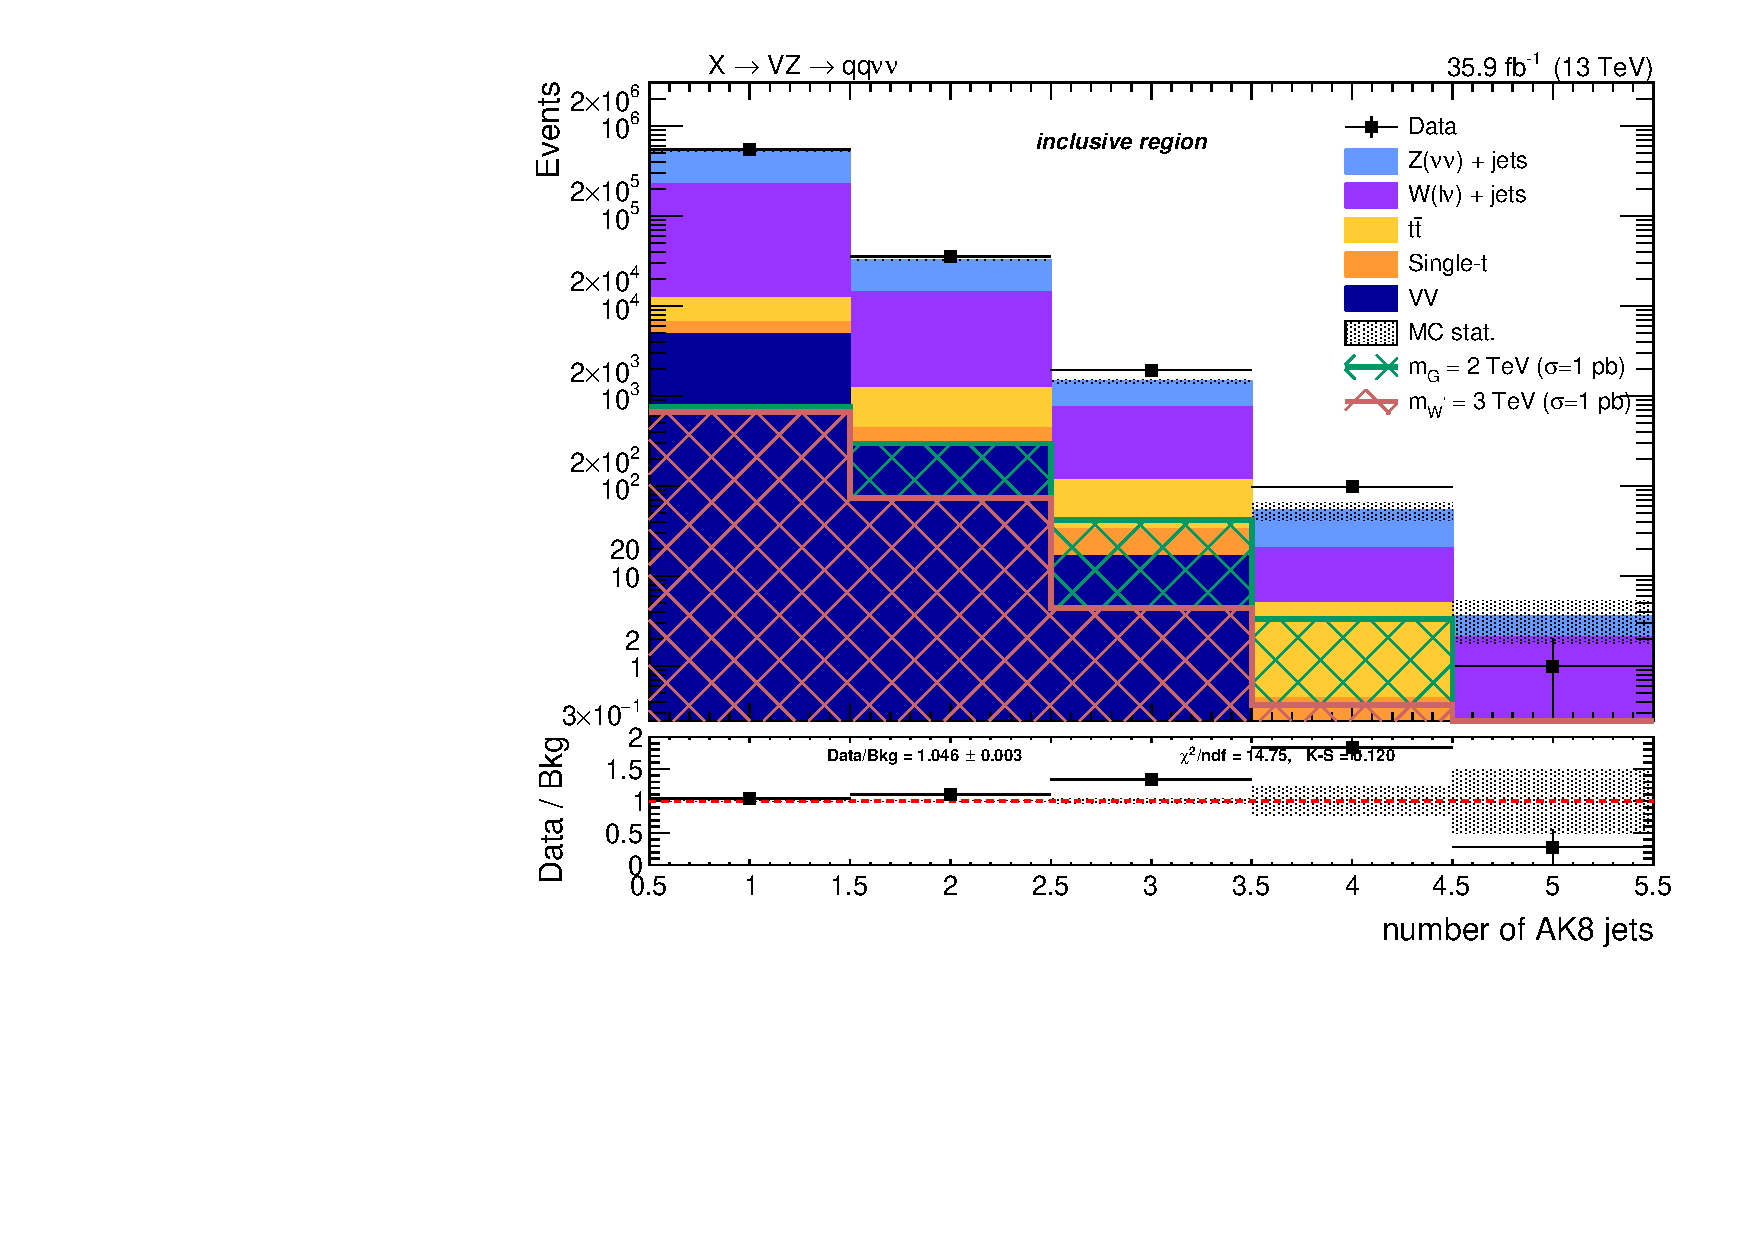
\includegraphics[width=0.495\textwidth]{plots/v9_thesis/XVZnnInc/nFatJets.pdf}  
    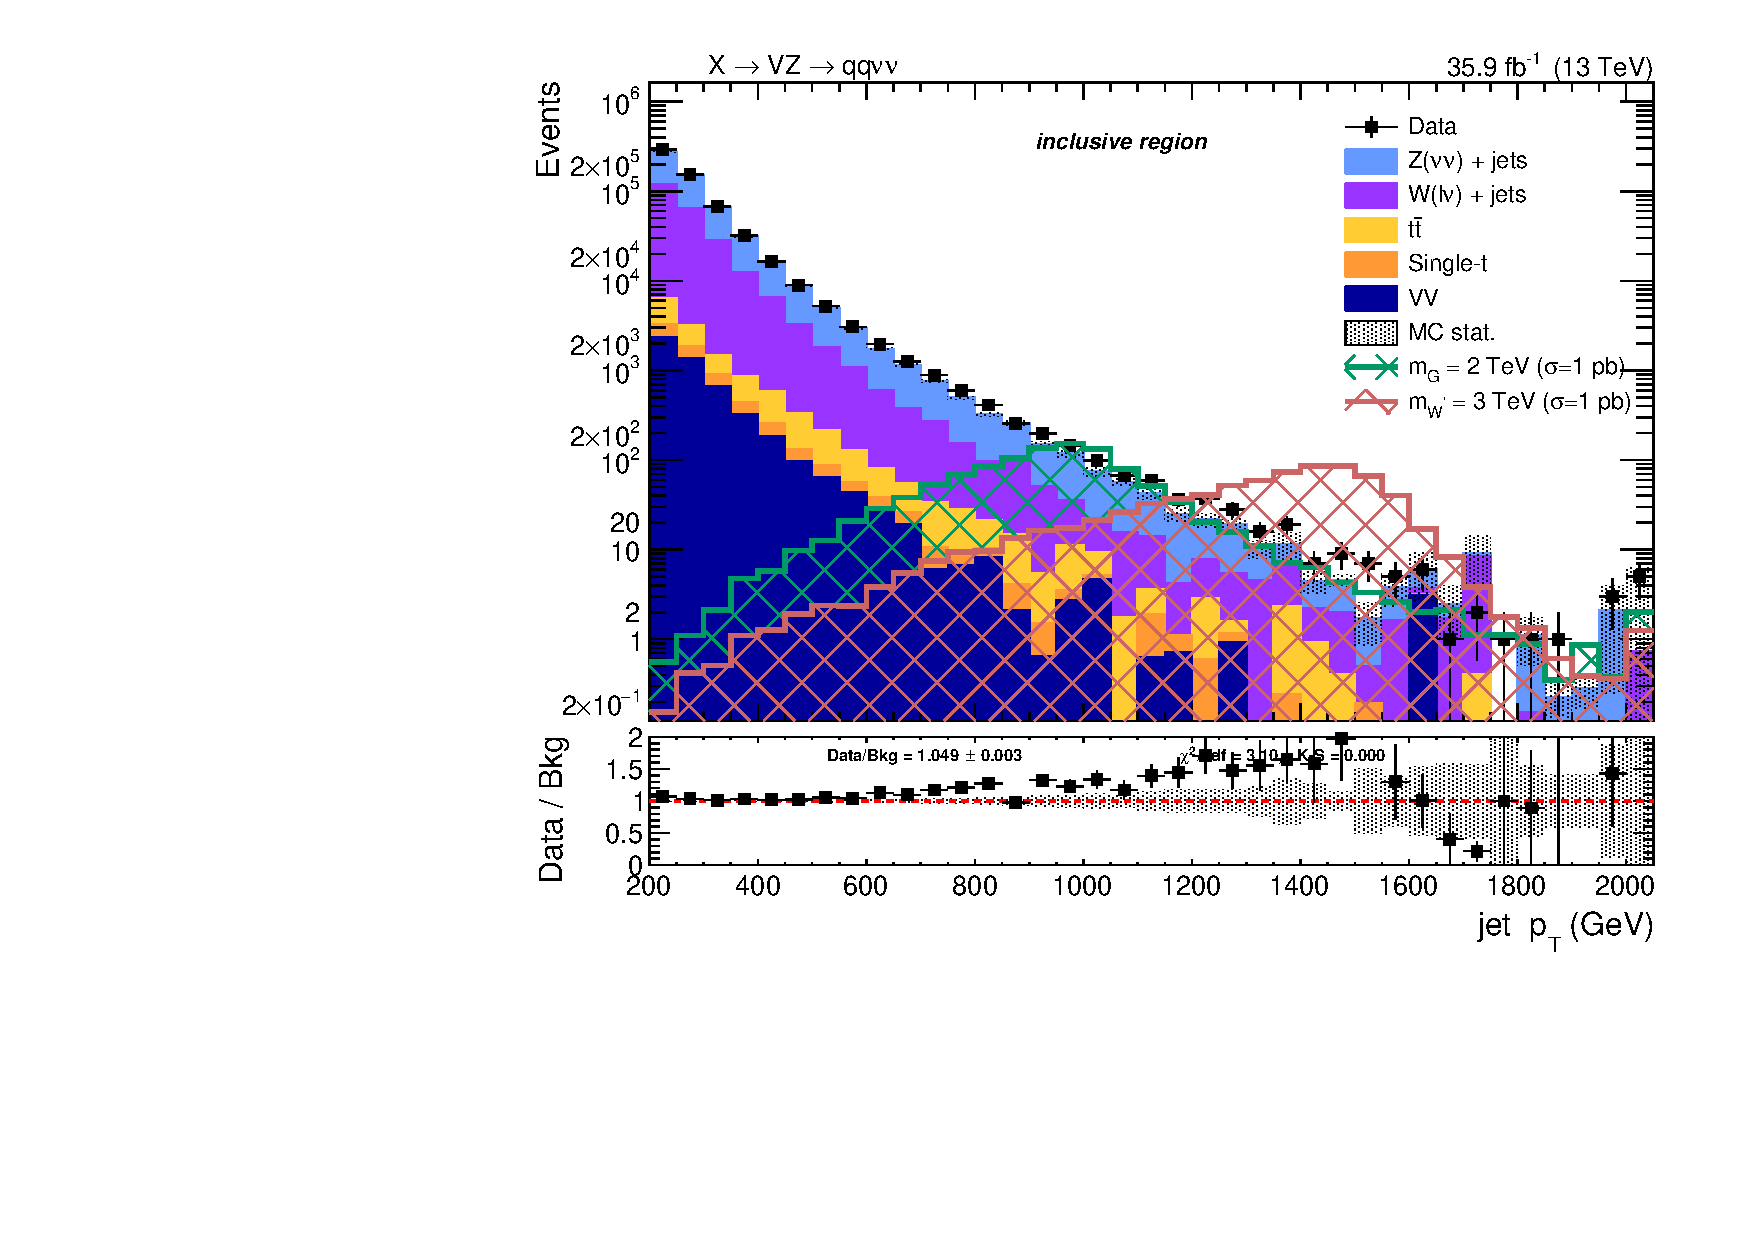
\includegraphics[width=0.495\textwidth]{plots/v9_thesis/XVZnnInc/FatJet1_pt.pdf}
    
    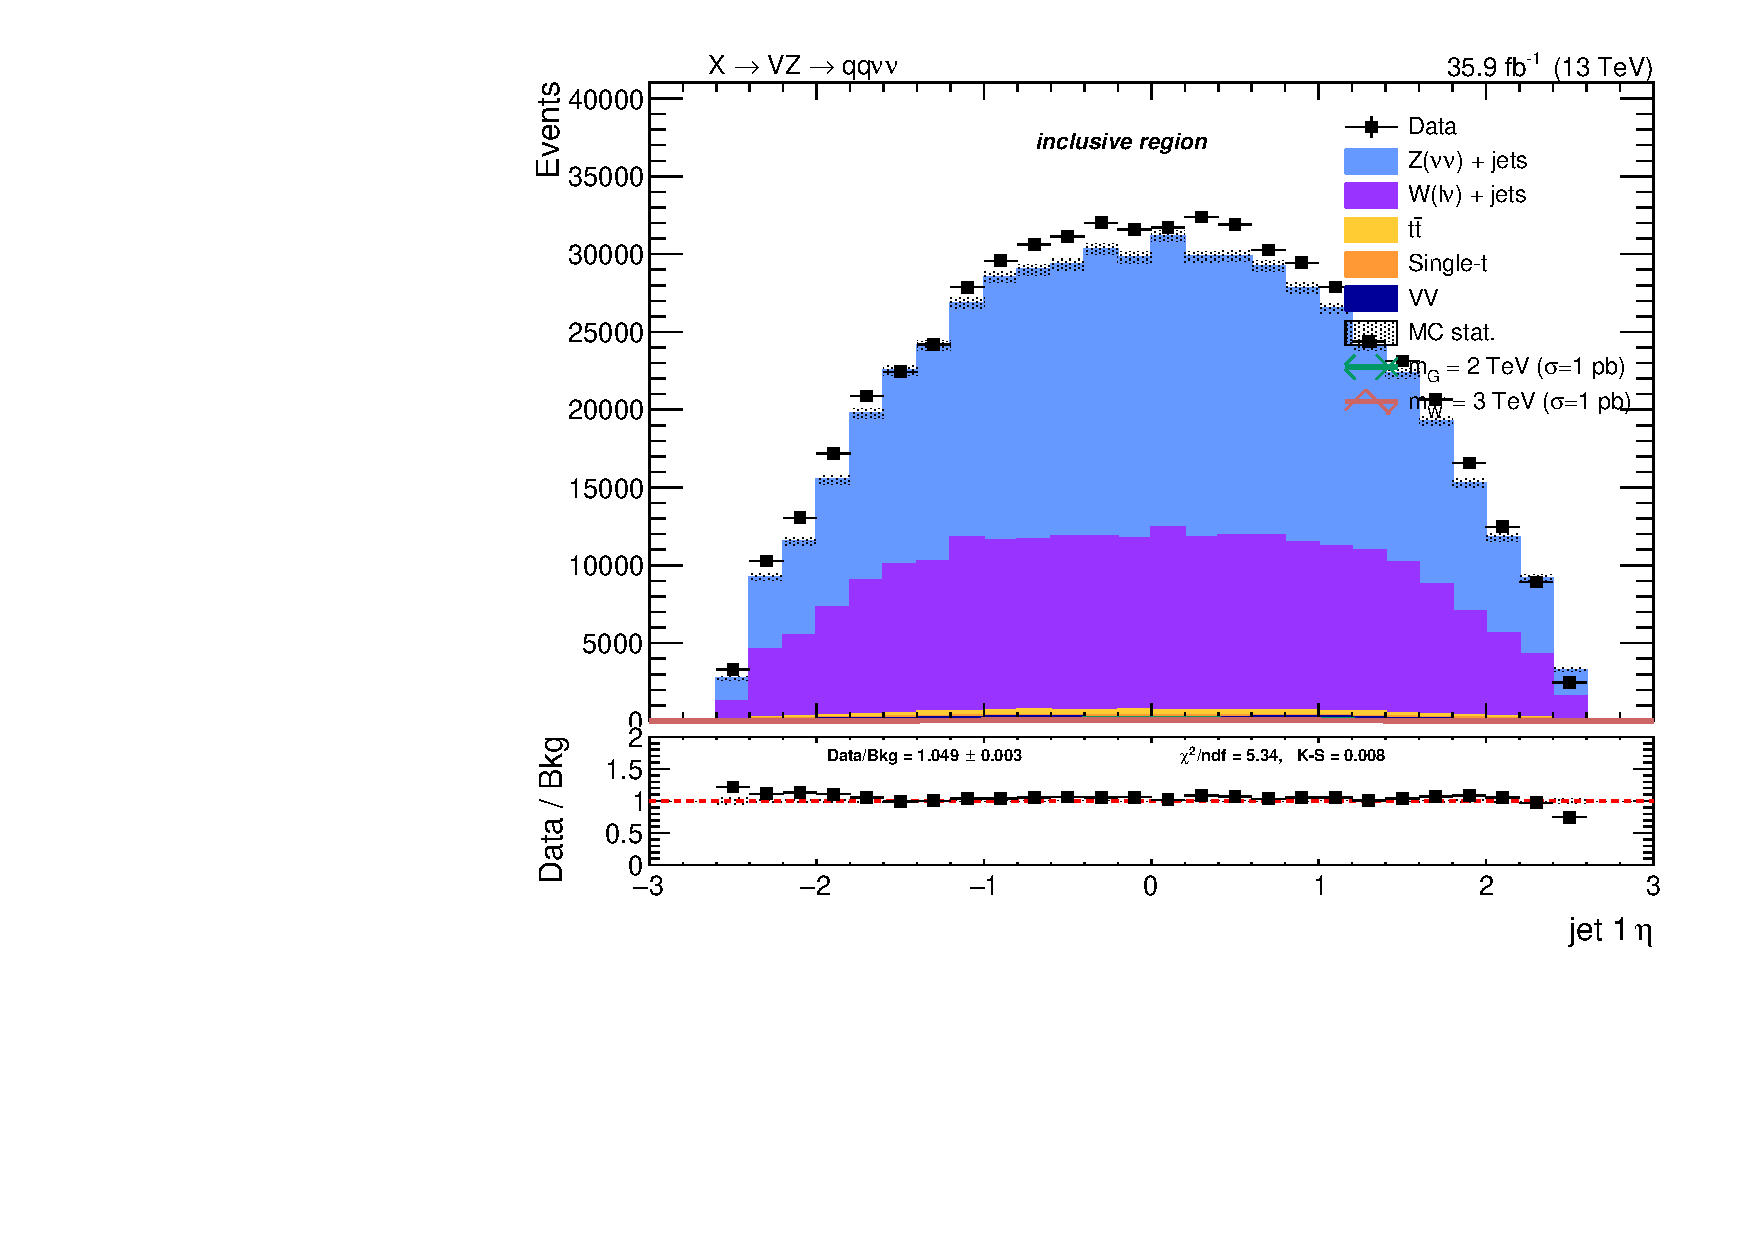
\includegraphics[width=0.495\textwidth]{plots/v9_thesis/XVZnnInc/FatJet1_eta.pdf}
    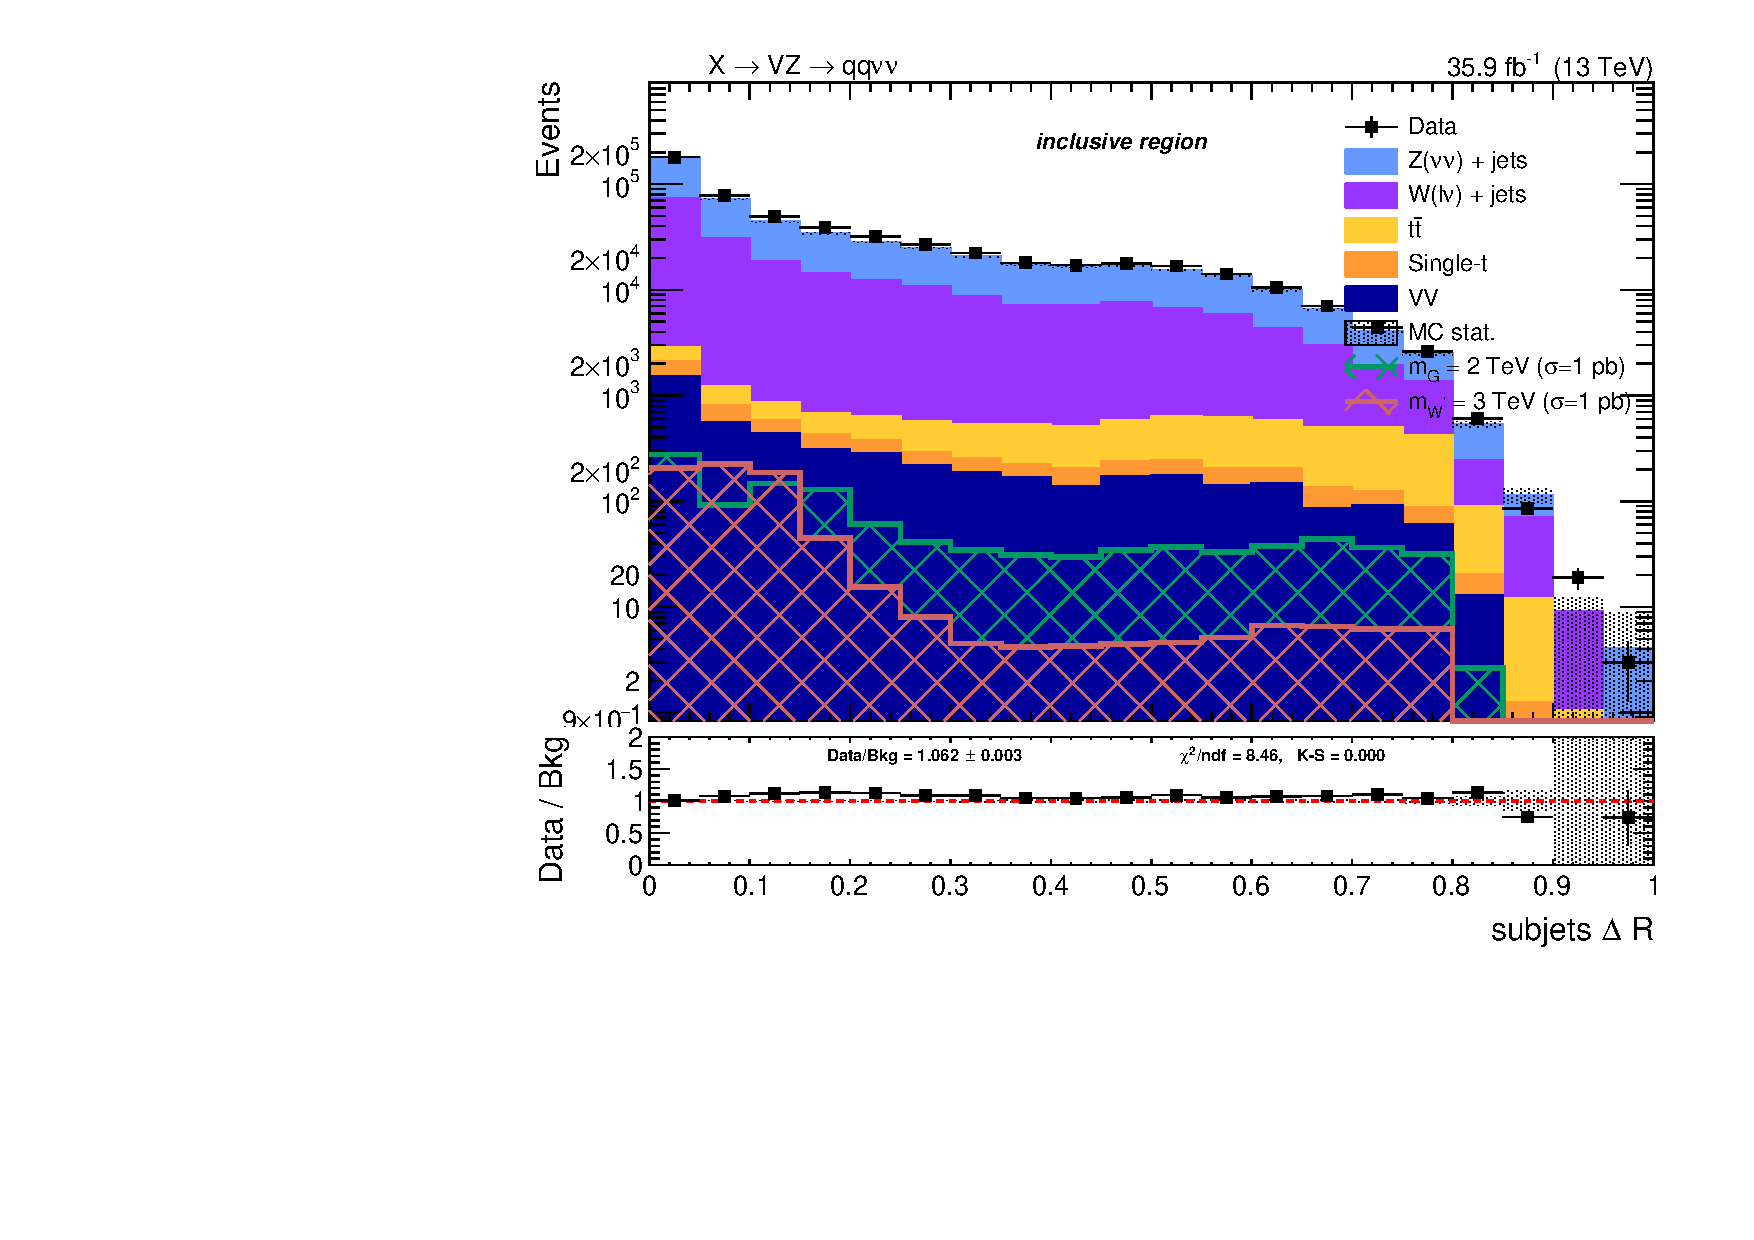
\includegraphics[width=0.495\textwidth]{plots/v9_thesis/XVZnnInc/FatJet1_dR.pdf}

    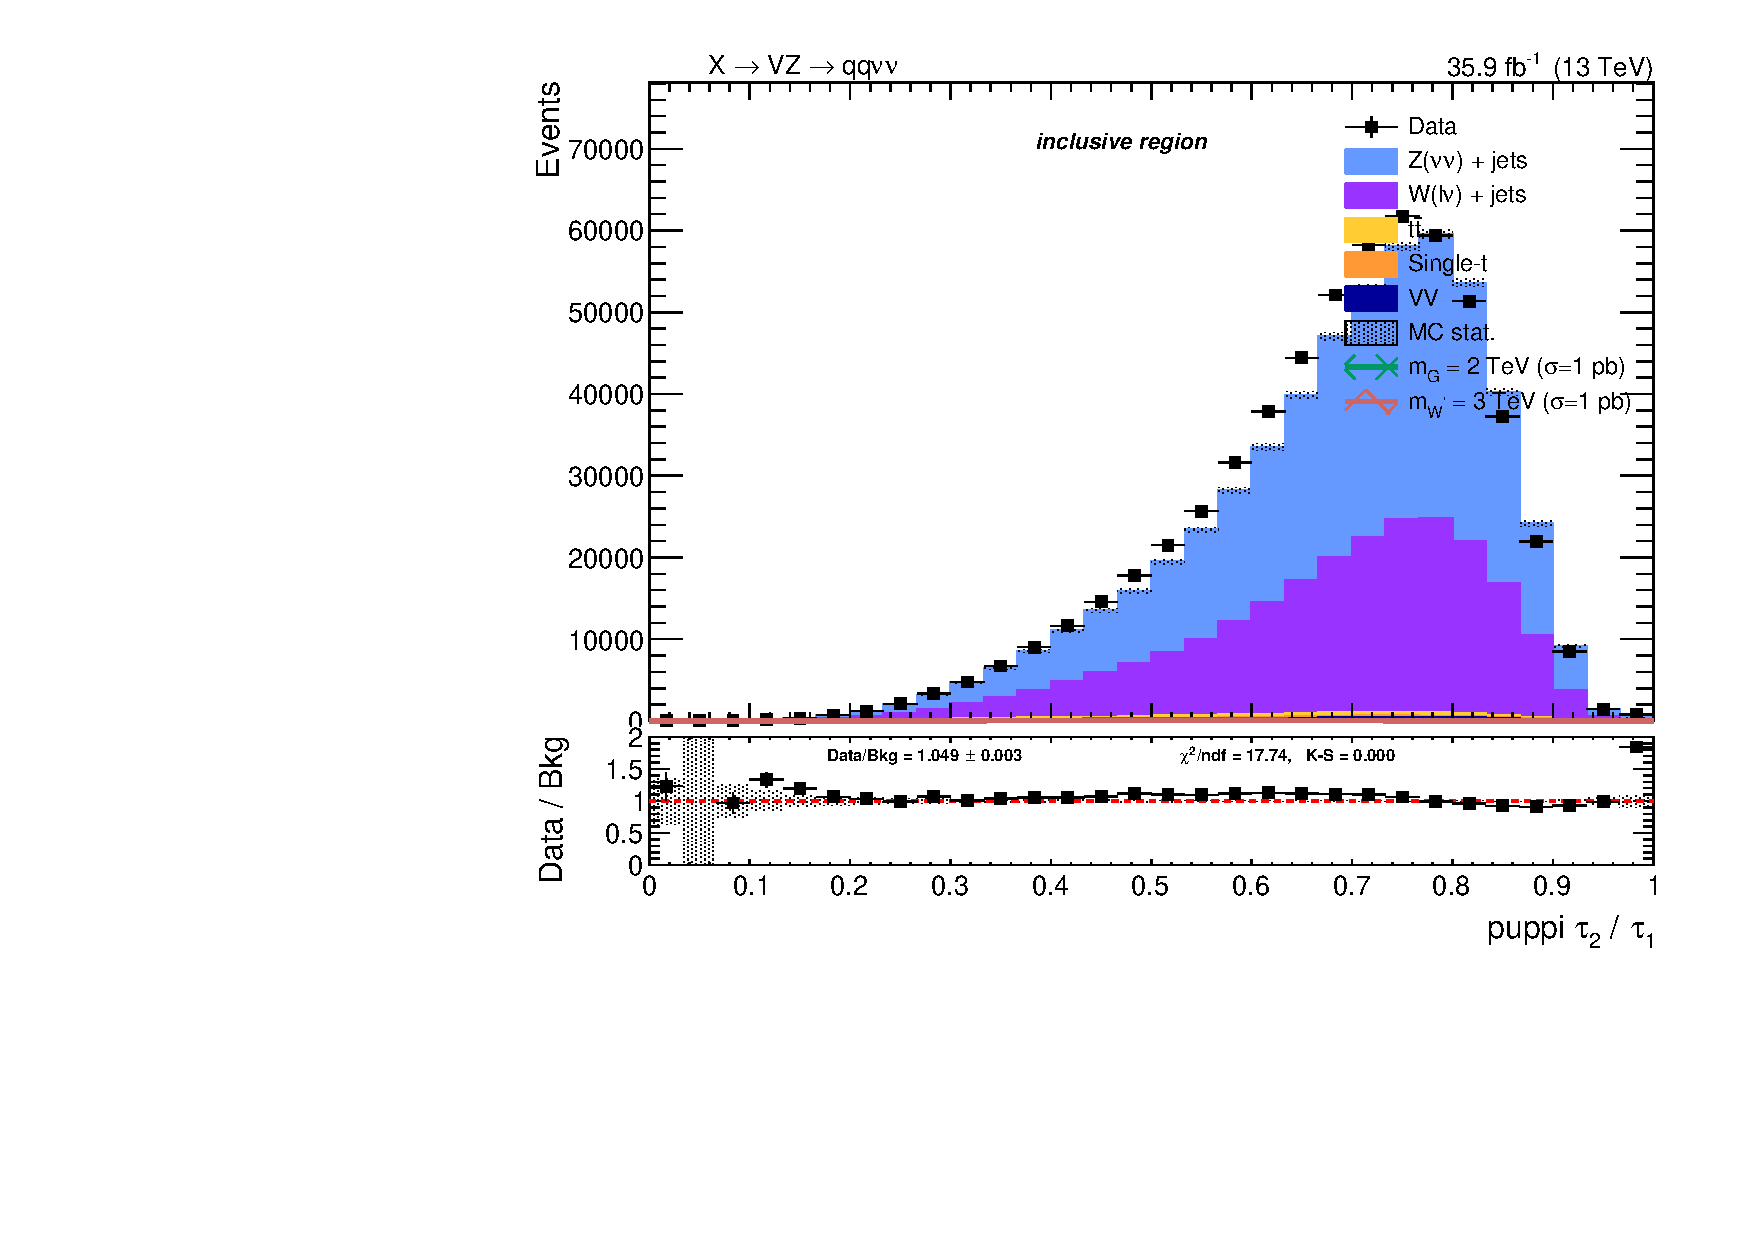
\includegraphics[width=0.495\textwidth]{plots/v9_thesis/XVZnnInc/FatJet1_puppiTau21.pdf}
    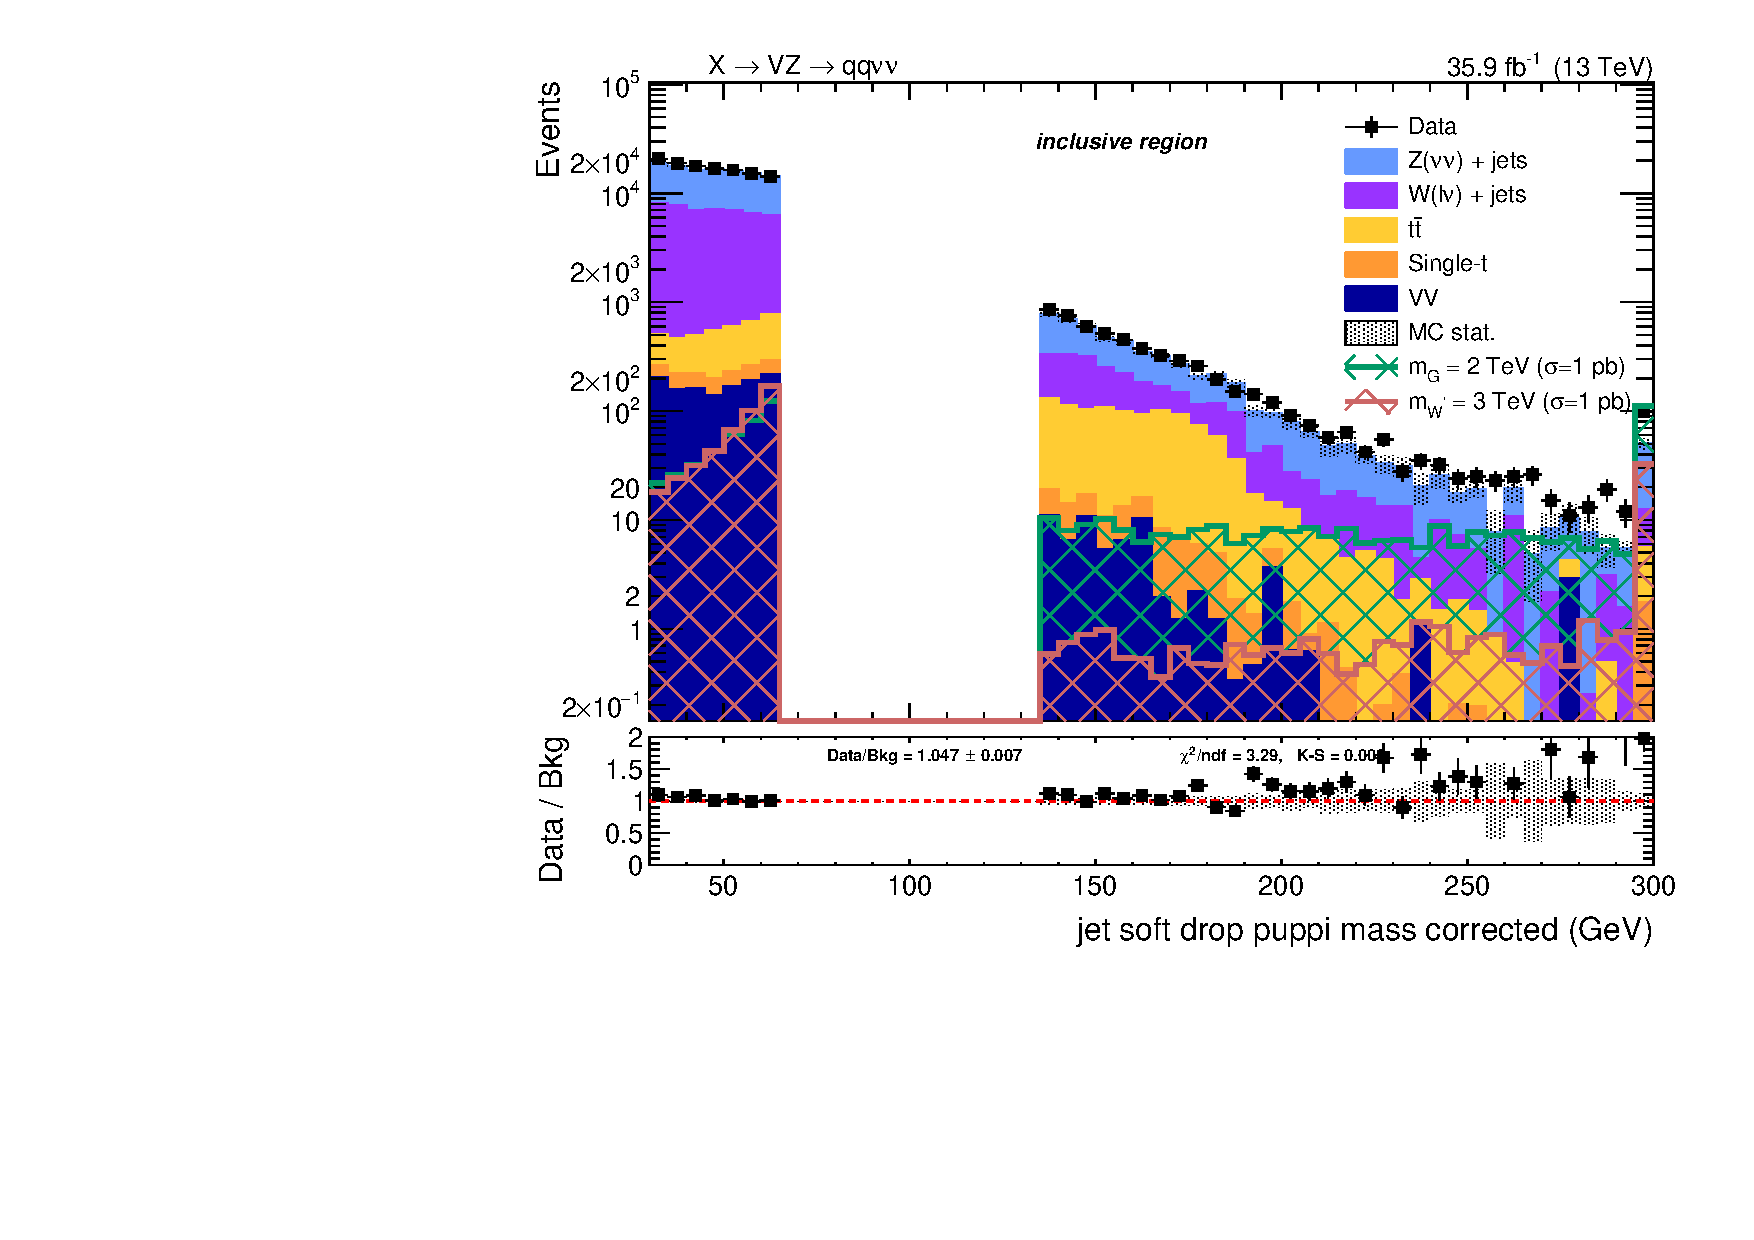
\includegraphics[width=0.495\textwidth]{plots/v9_thesis/XVZnnInc/FatJet1_softdropPuppiMassCorr.pdf}

    \caption{Top: number of AK8 jets in the event (left) and \V jet candidate \pt (right). Center: \V jet candidate $\eta$ (left) and angular separation $\Delta R$ between the constituents leading subjets (right). Bottom: \V jet candidate $\tau_{21}$ subjettiness after PUPPI correction (left) and \V jet candidate soft drop PUPPI mass (right). Events are selected with the \emph{inclusive} selection, and simulated backgrounds are normalized to luminosity.}
\label{fig:plot_uno}
  \end{center}
\end{figure}

\clearpage

\begin{figure}[!htb]
  \begin{center}  
    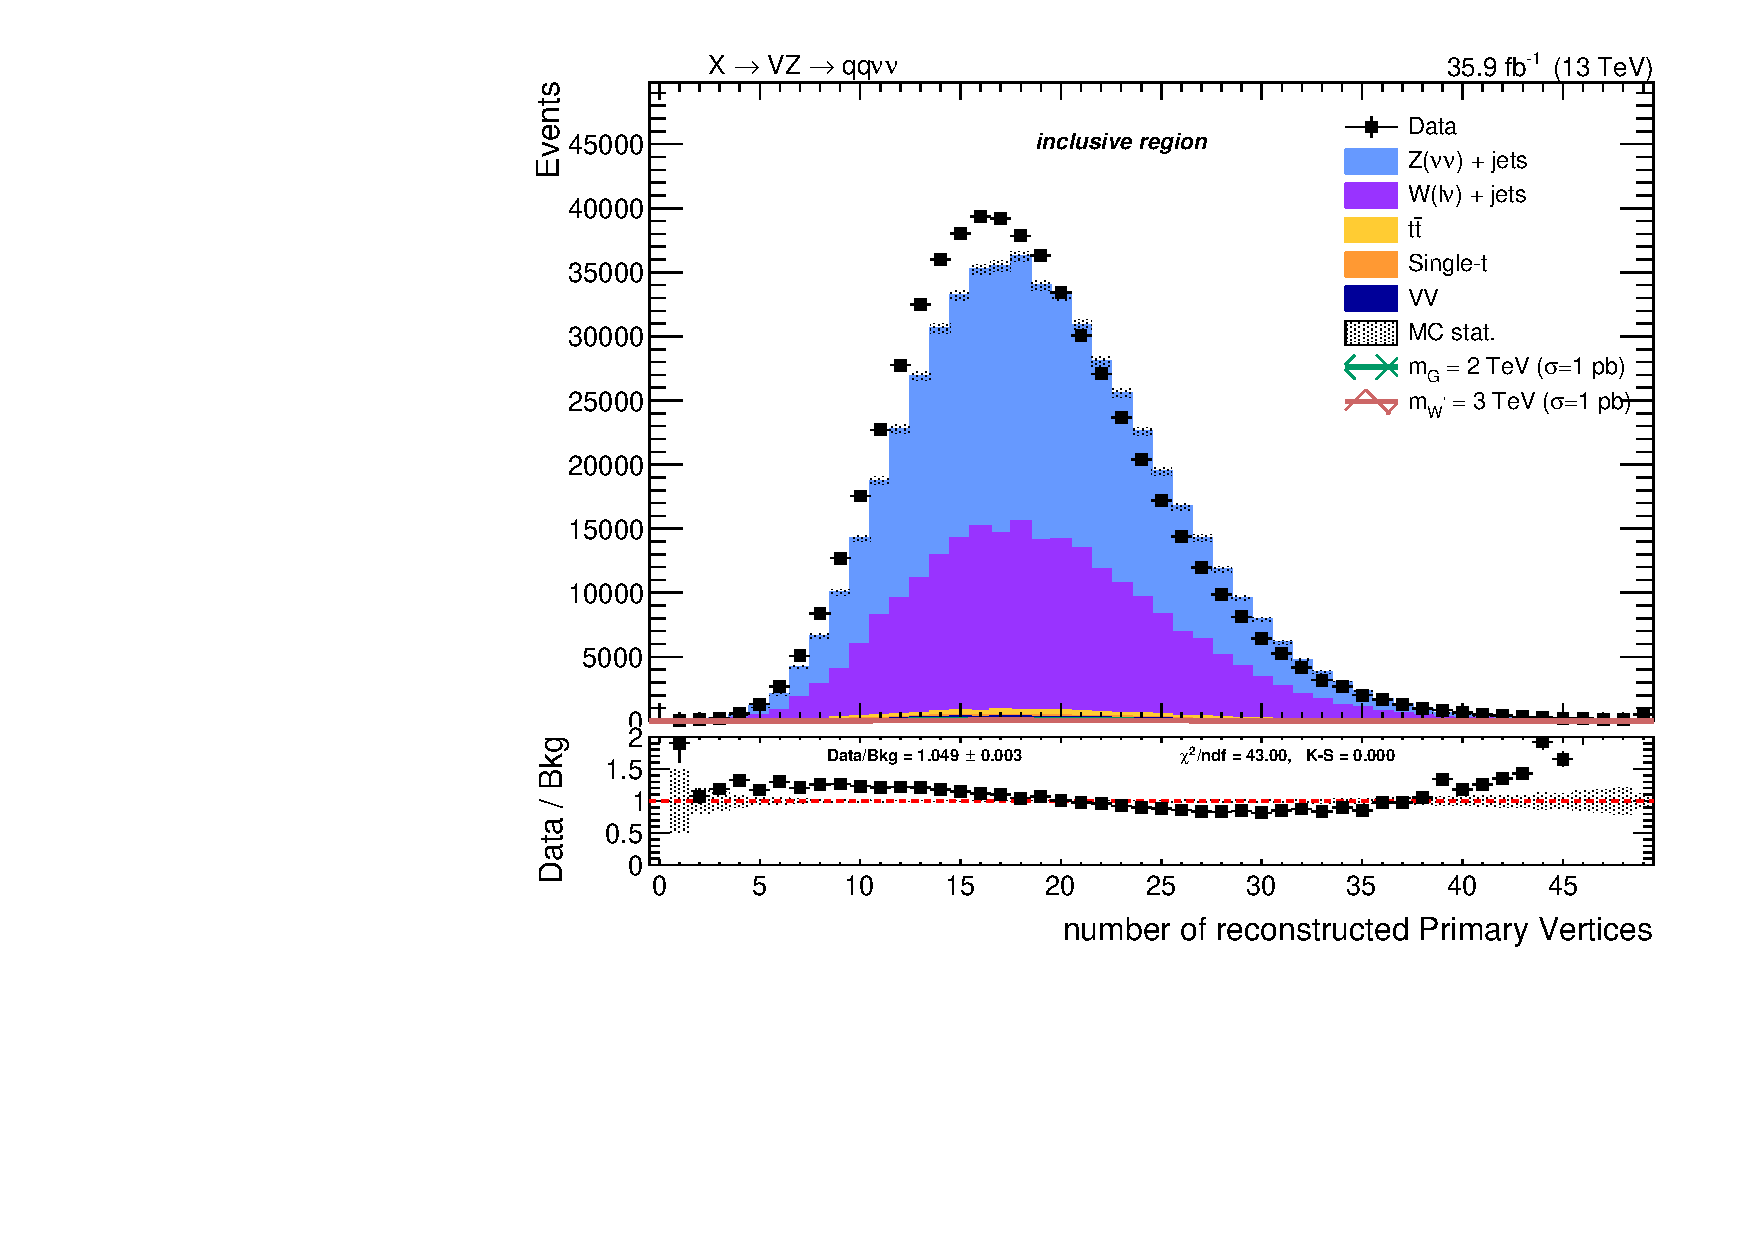
\includegraphics[width=0.495\textwidth]{plots/v9_thesis/XVZnnInc/nPV.pdf}
    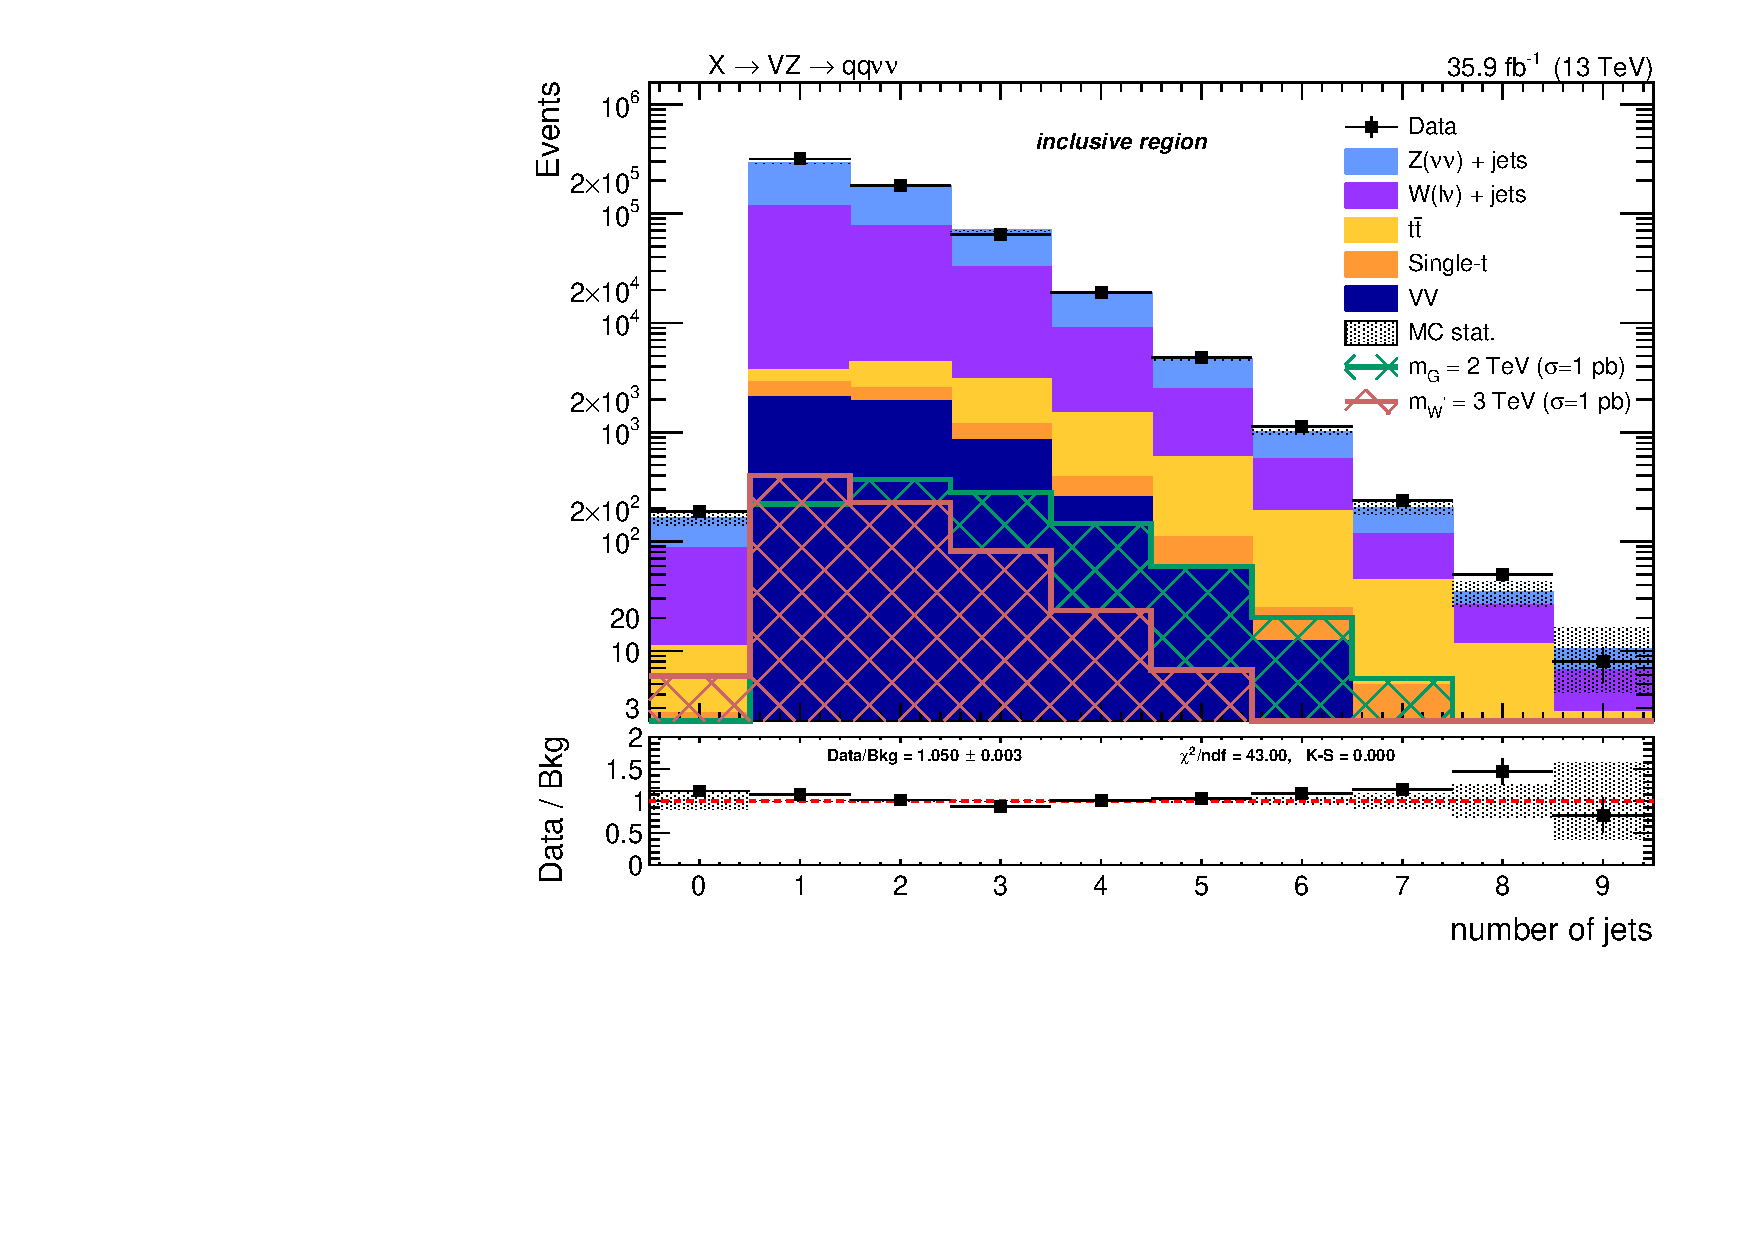
\includegraphics[width=0.495\textwidth]{plots/v9_thesis/XVZnnInc/nJets.pdf}

    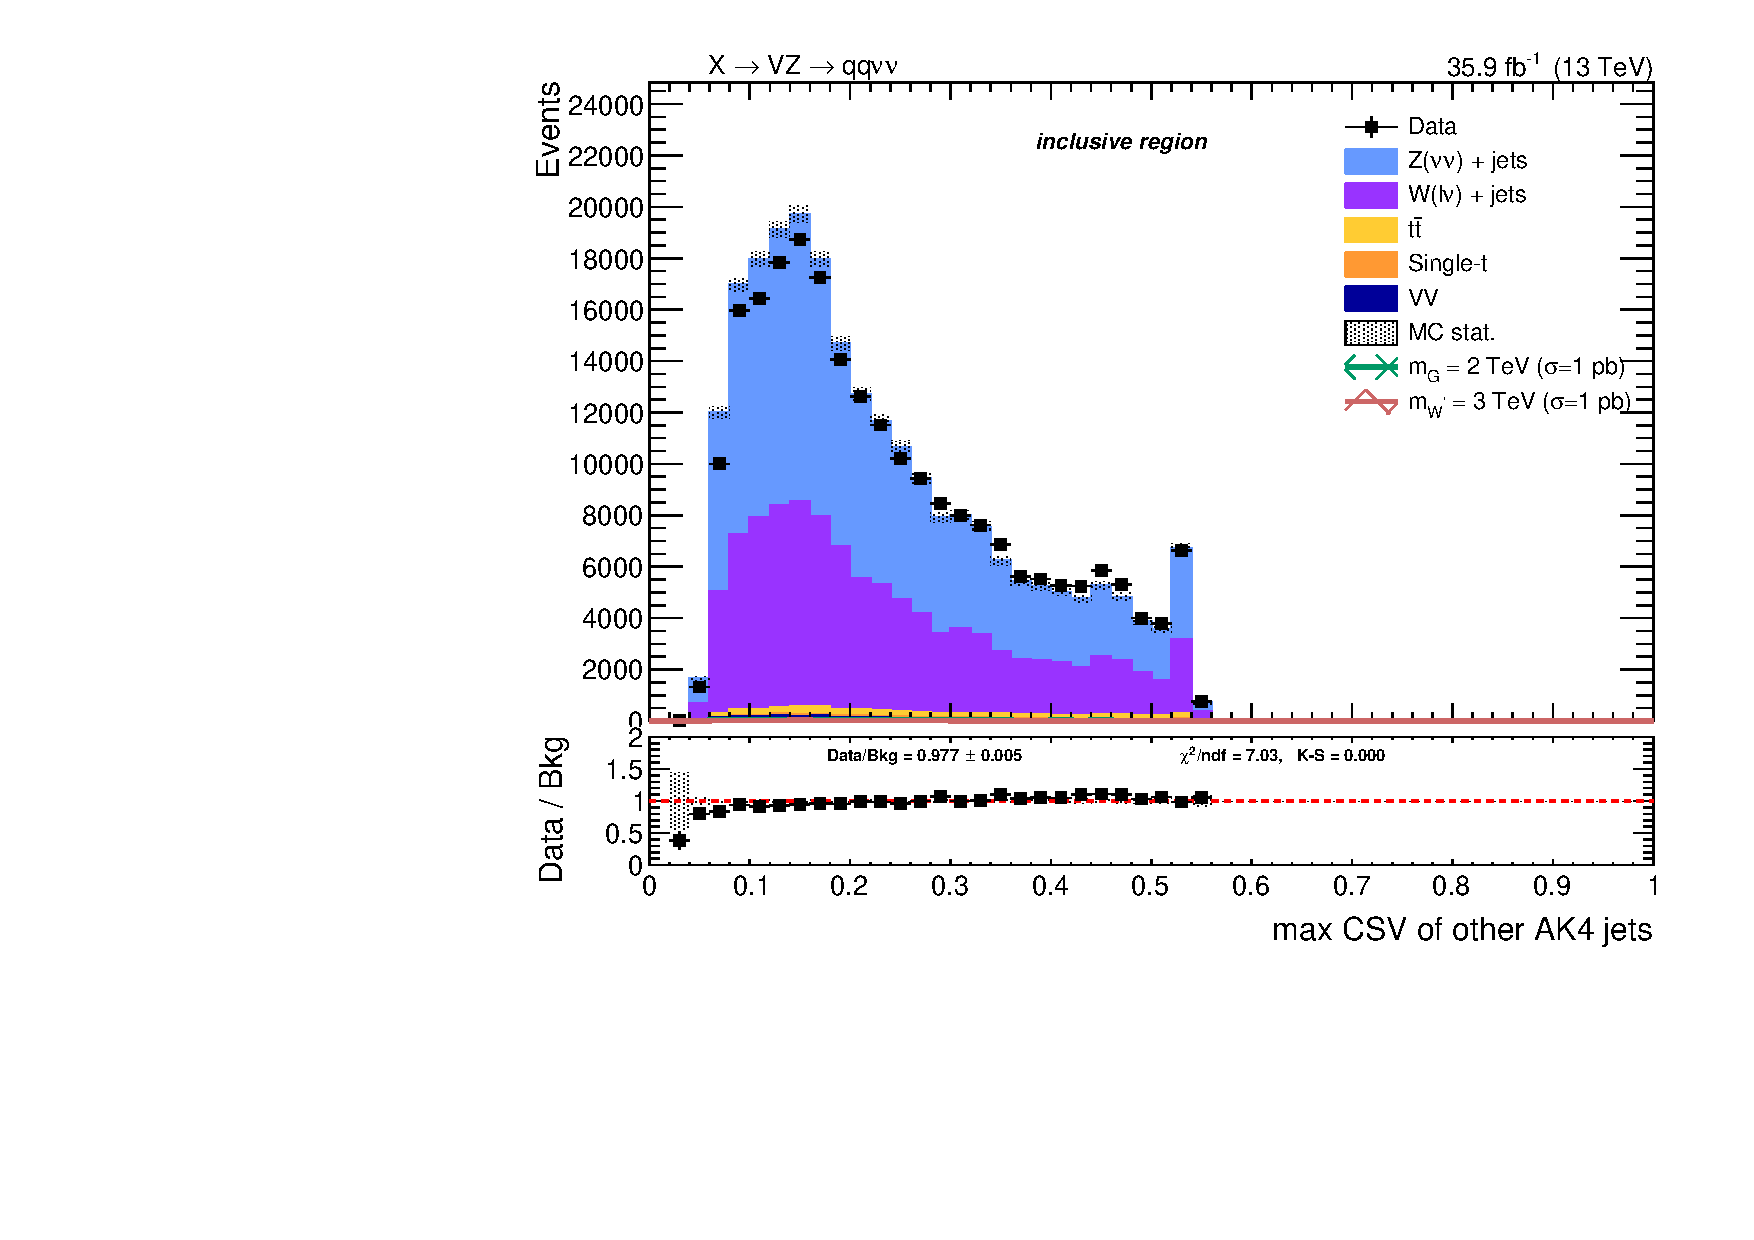
\includegraphics[width=0.495\textwidth]{plots/v9_thesis/XVZnnInc/MaxJetBTag.pdf}
    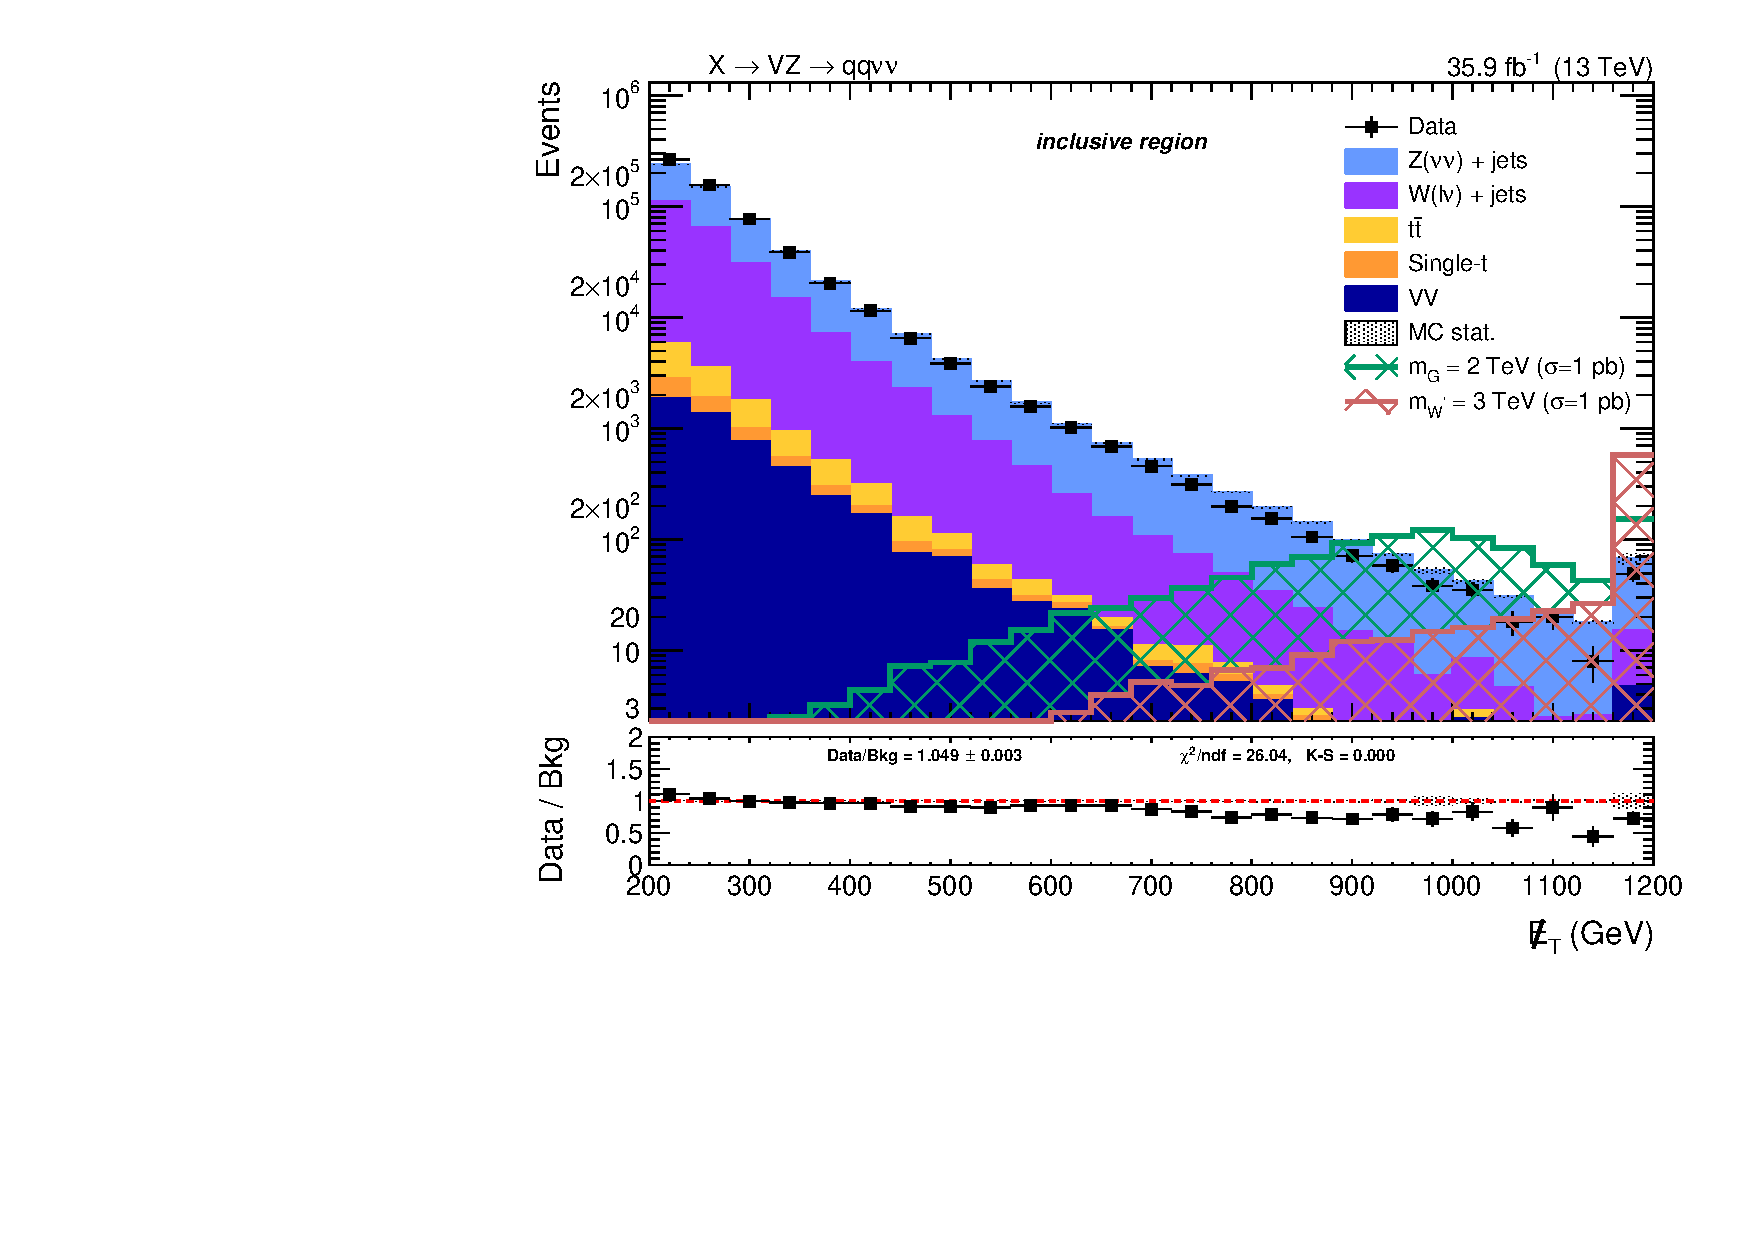
\includegraphics[width=0.495\textwidth]{plots/v9_thesis/XVZnnInc/MEt_pt.pdf}

    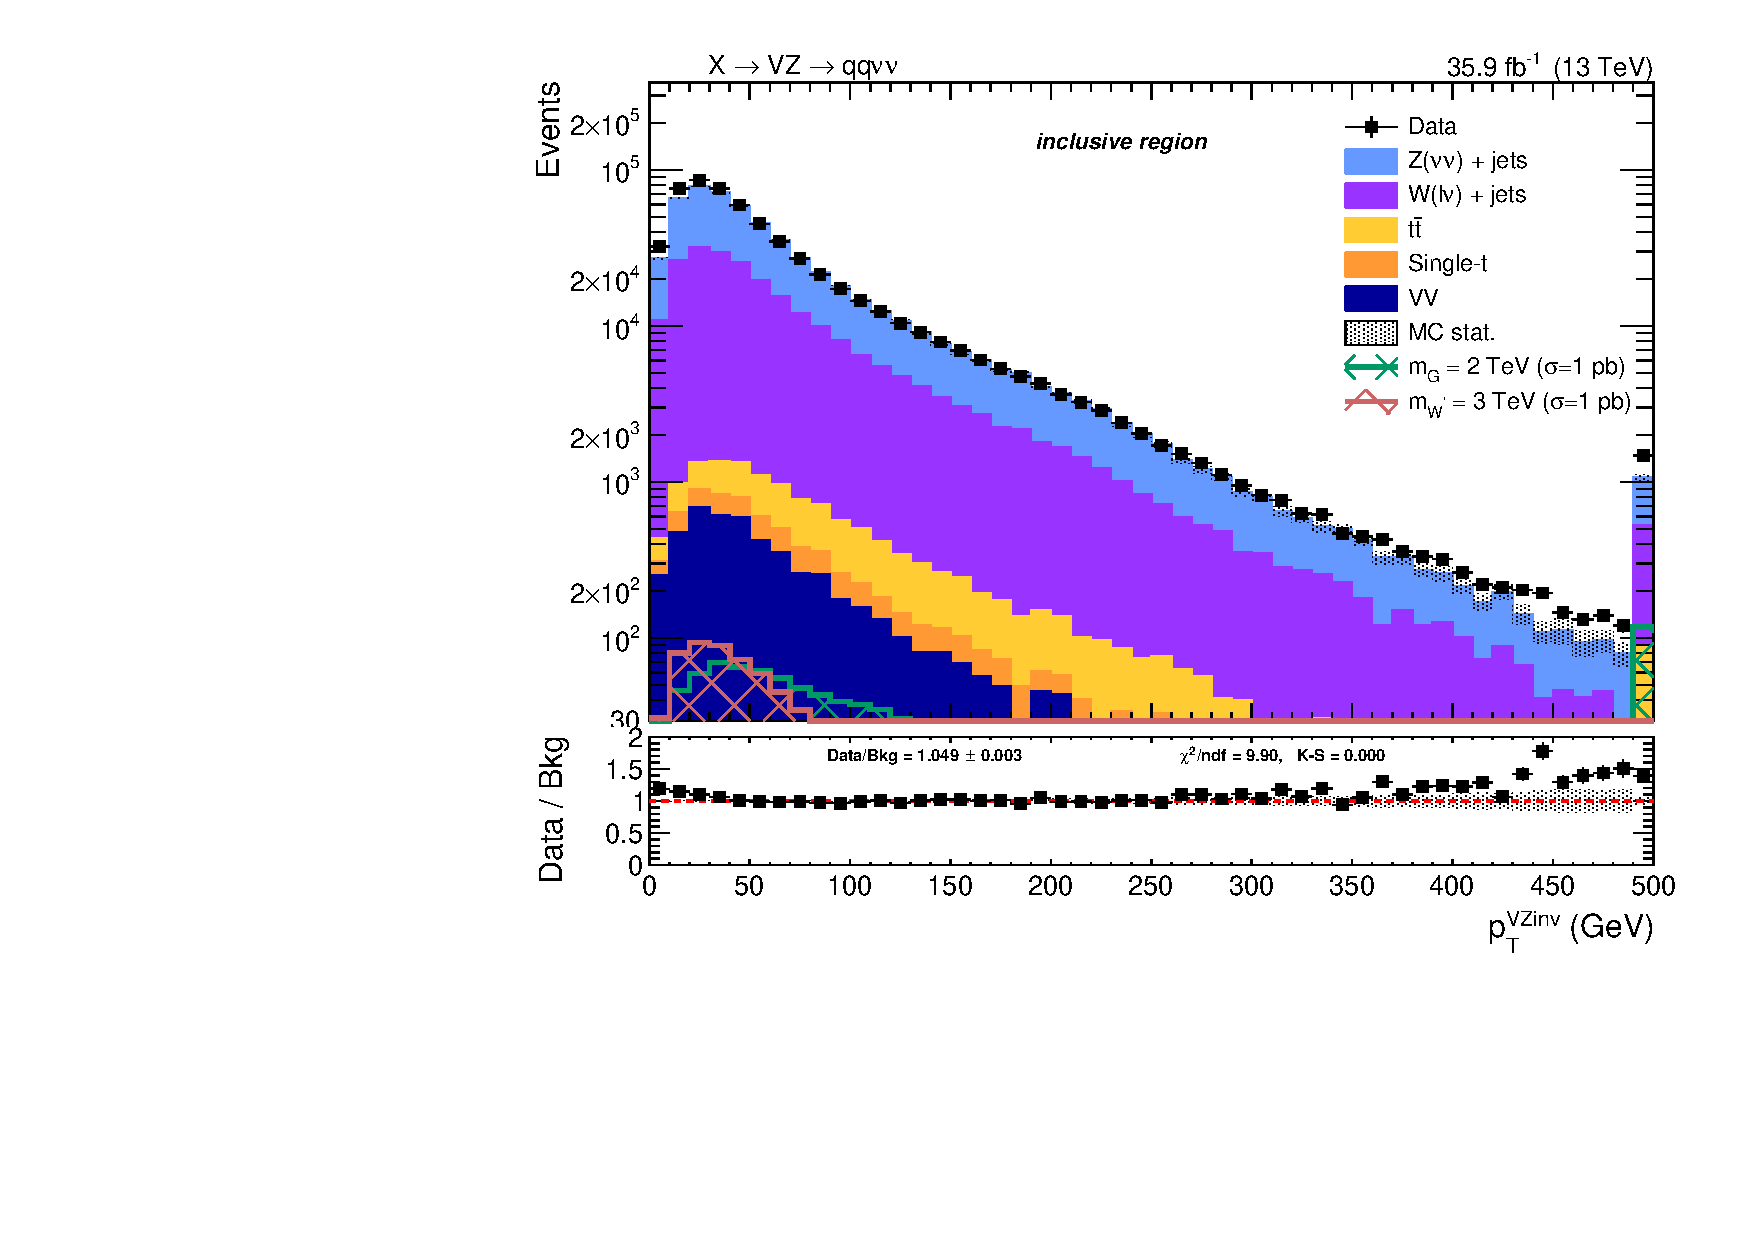
\includegraphics[width=0.495\textwidth]{plots/v9_thesis/XVZnnInc/X_pt.pdf}
    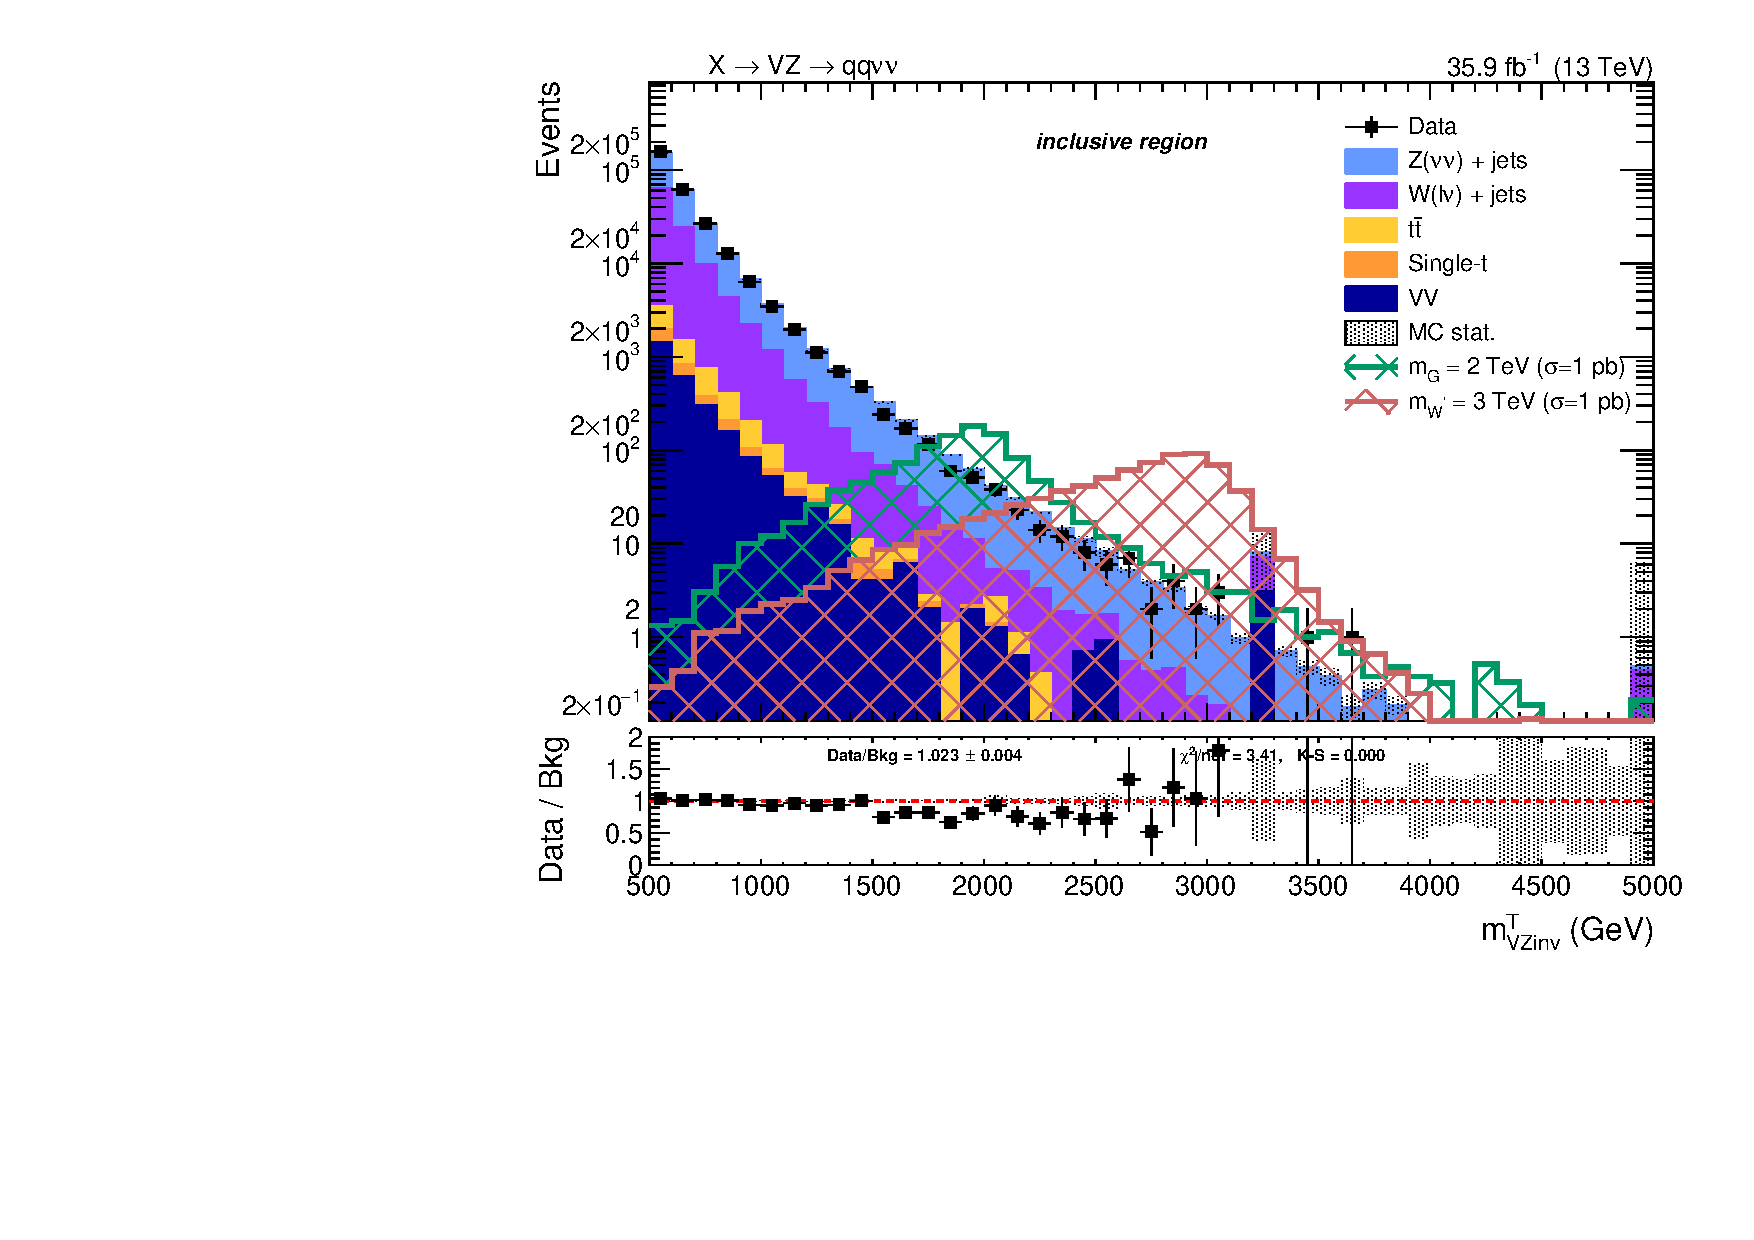
\includegraphics[width=0.495\textwidth]{plots/v9_thesis/XVZnnInc/X_tmass.pdf}

    \caption{Top: number of reconstructed primary vertices (left) and number of AK4 jets in the event (right). Center: distribution of the b-tagging multivariate discriminant for the AK4 jets not included in the \V jet cone (left) and \MET distribution (right). Bottom: \pt of the \VZ candidate (left) and transverse mass of the \VZ candidate (right). Events are selected with the \emph{inclusive} selection, and simulated backgrounds are normalized to luminosity.}
%\label{fig:XZhll_N}
  \end{center}
\end{figure}

\clearpage

%plot scelti
%sideband lp

\begin{figure}[!htb]
  \begin{center}
    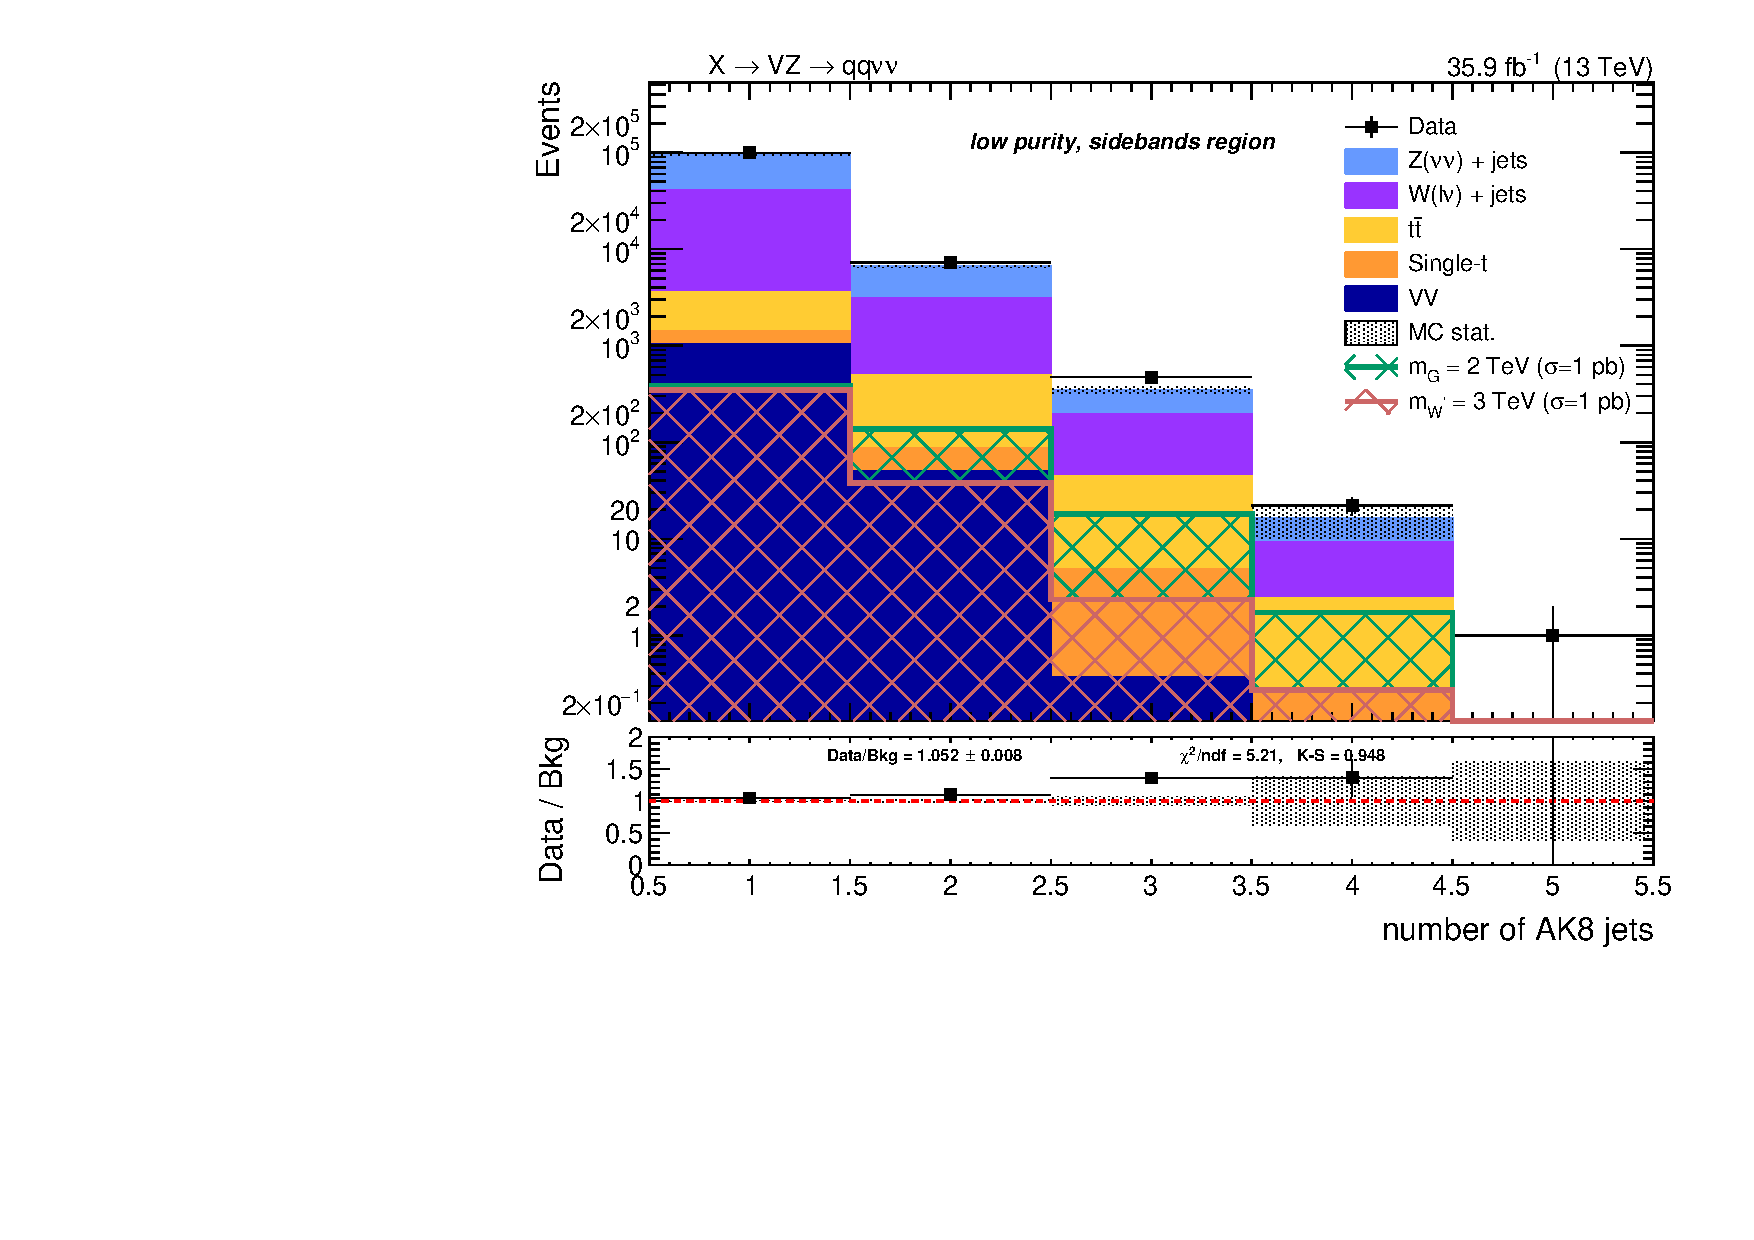
\includegraphics[width=0.495\textwidth]{plots/v9_thesis/XVZnnlpSB/nFatJets.pdf}  
    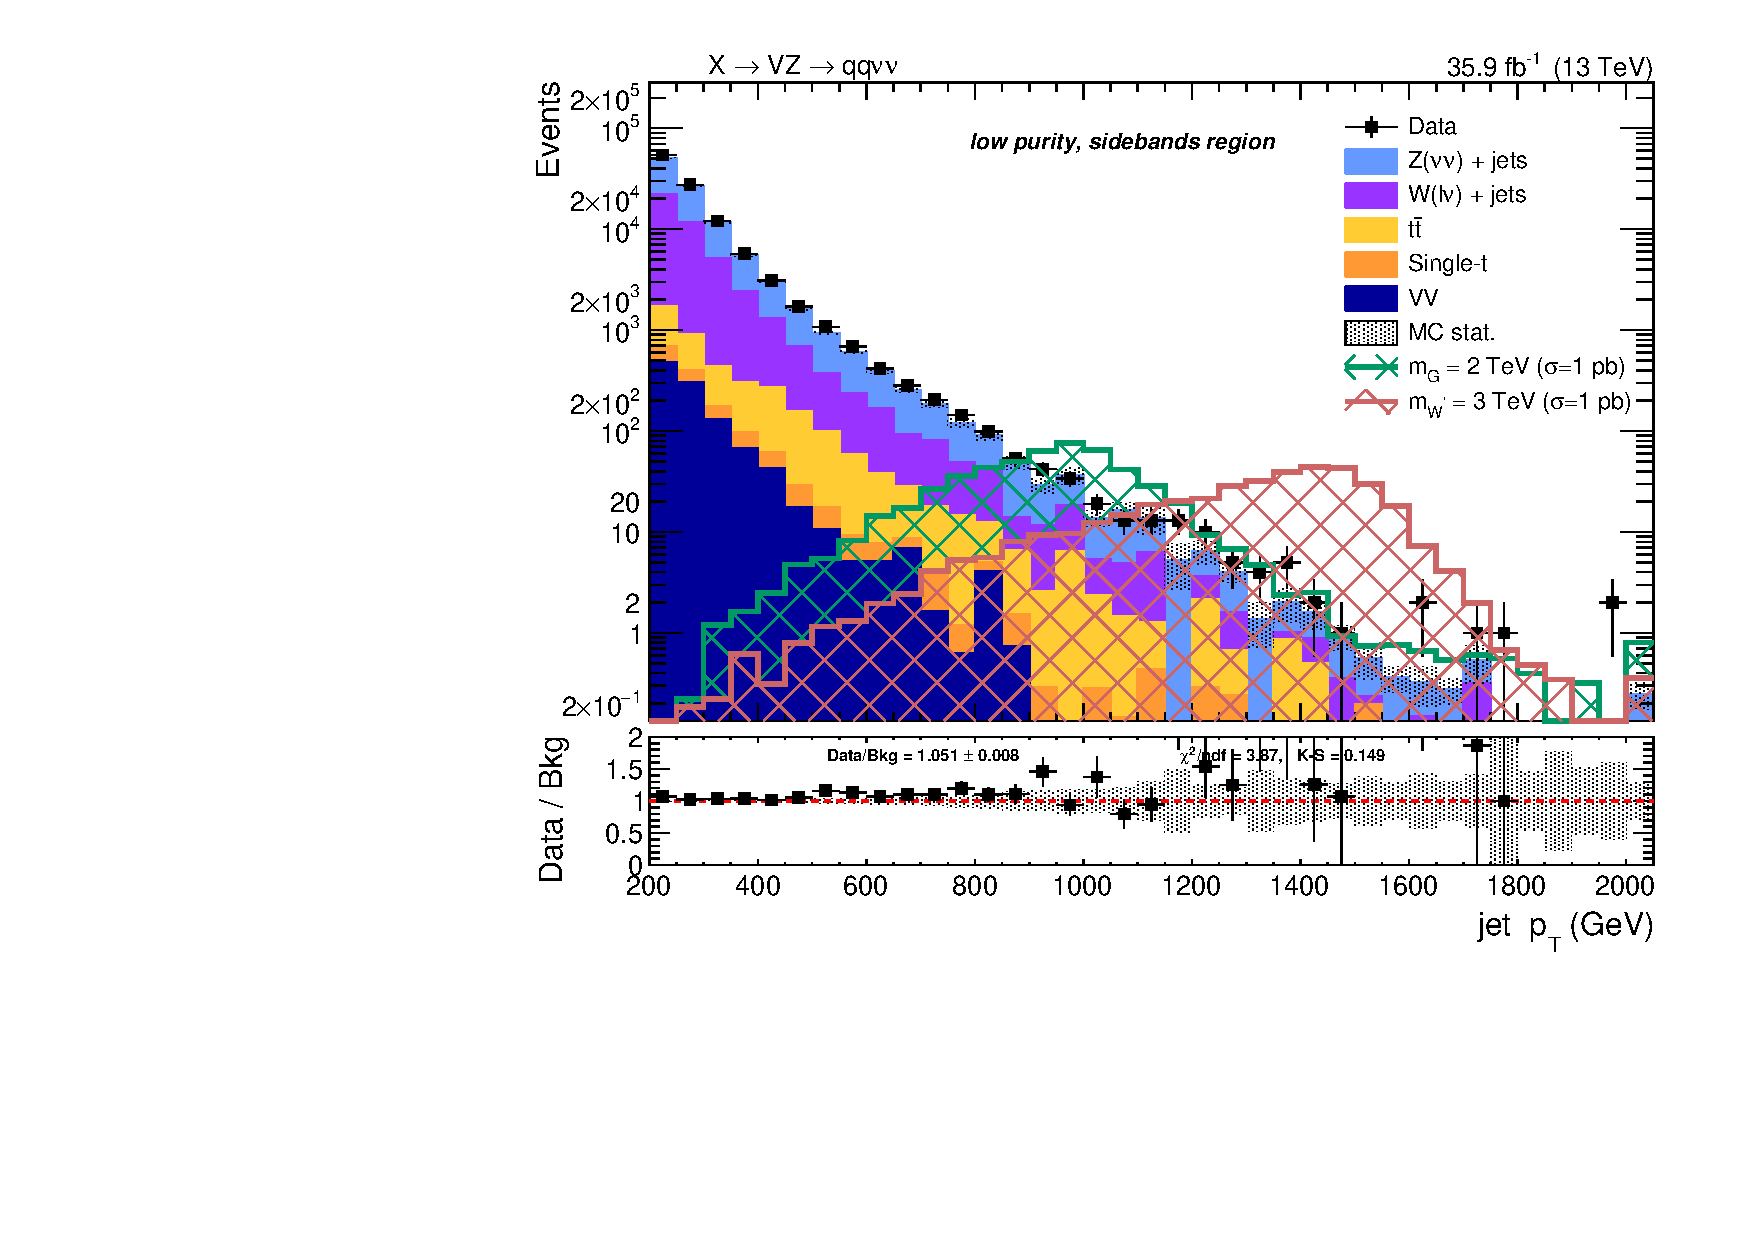
\includegraphics[width=0.495\textwidth]{plots/v9_thesis/XVZnnlpSB/FatJet1_pt.pdf}
    
    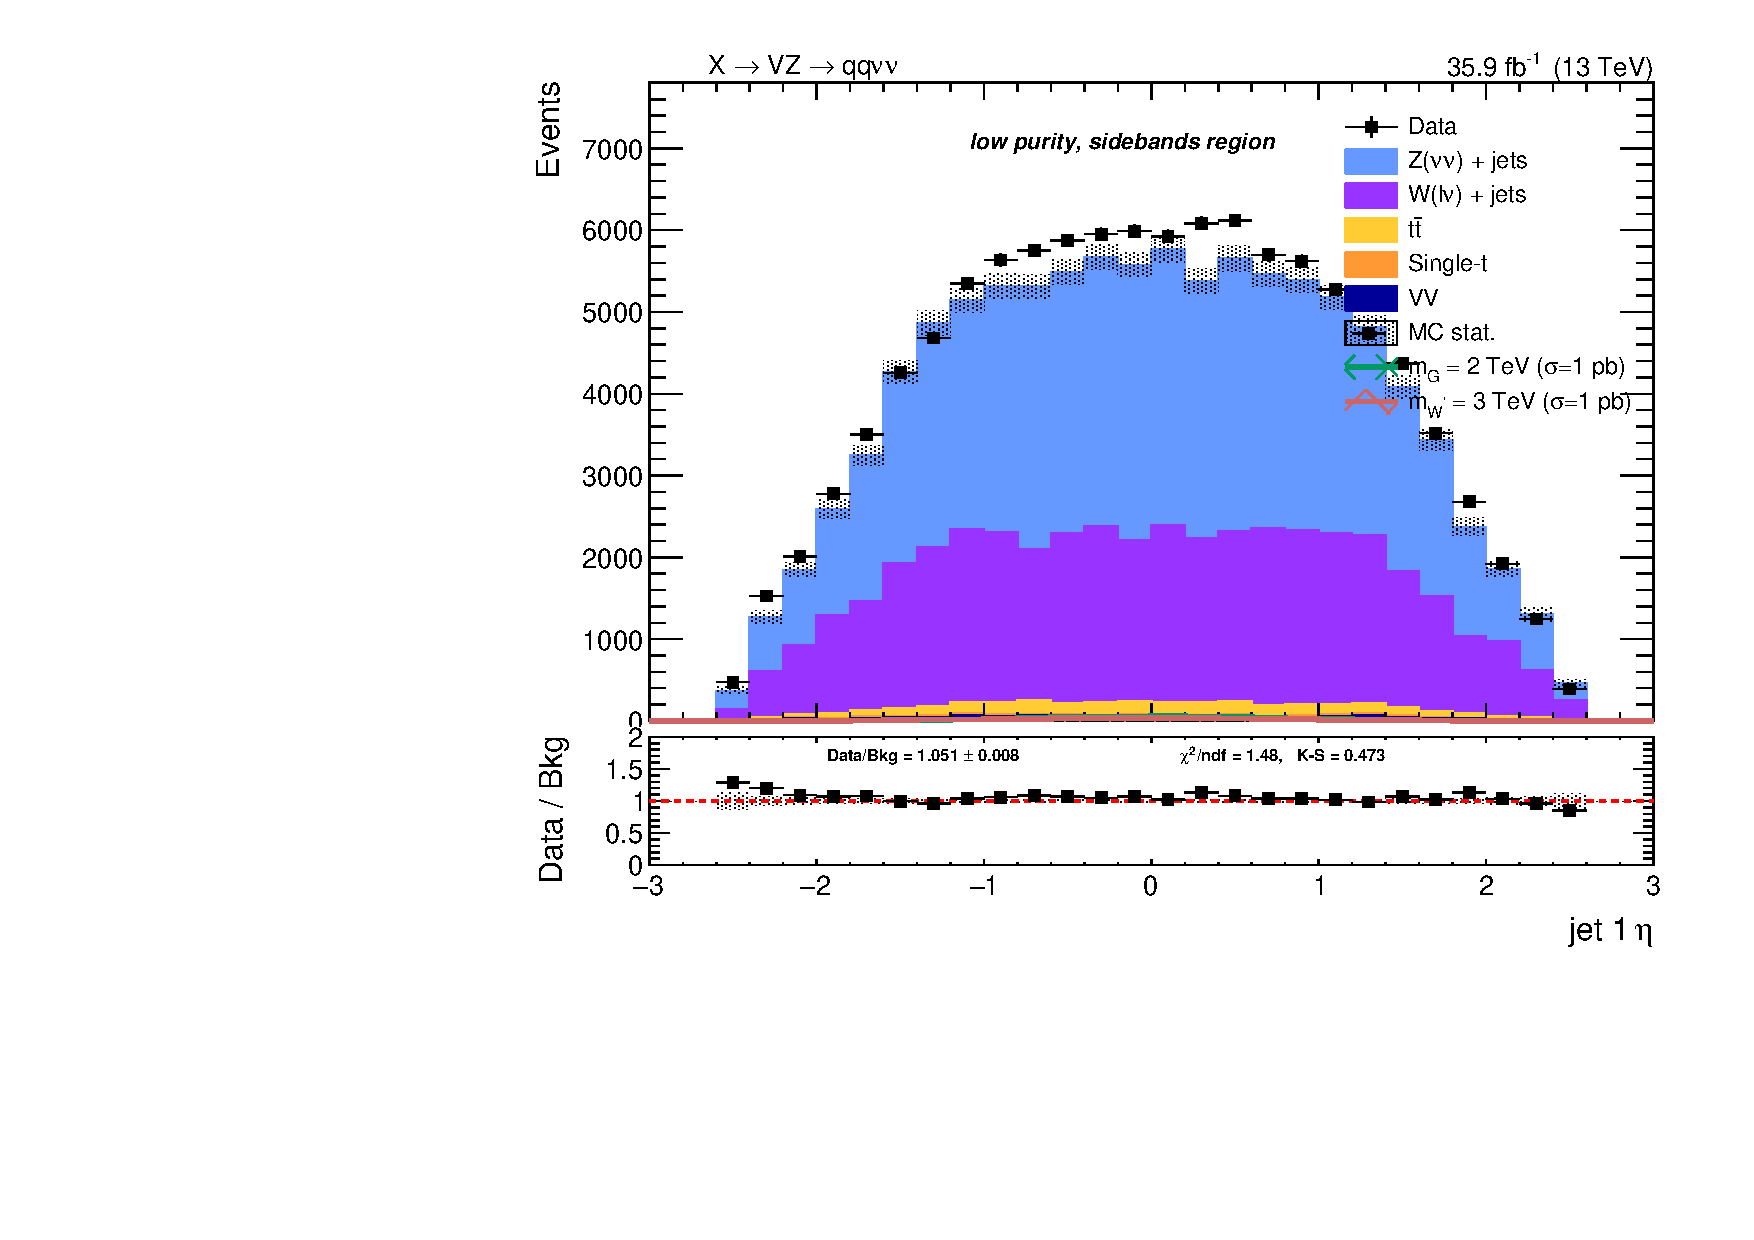
\includegraphics[width=0.495\textwidth]{plots/v9_thesis/XVZnnlpSB/FatJet1_eta.pdf}
    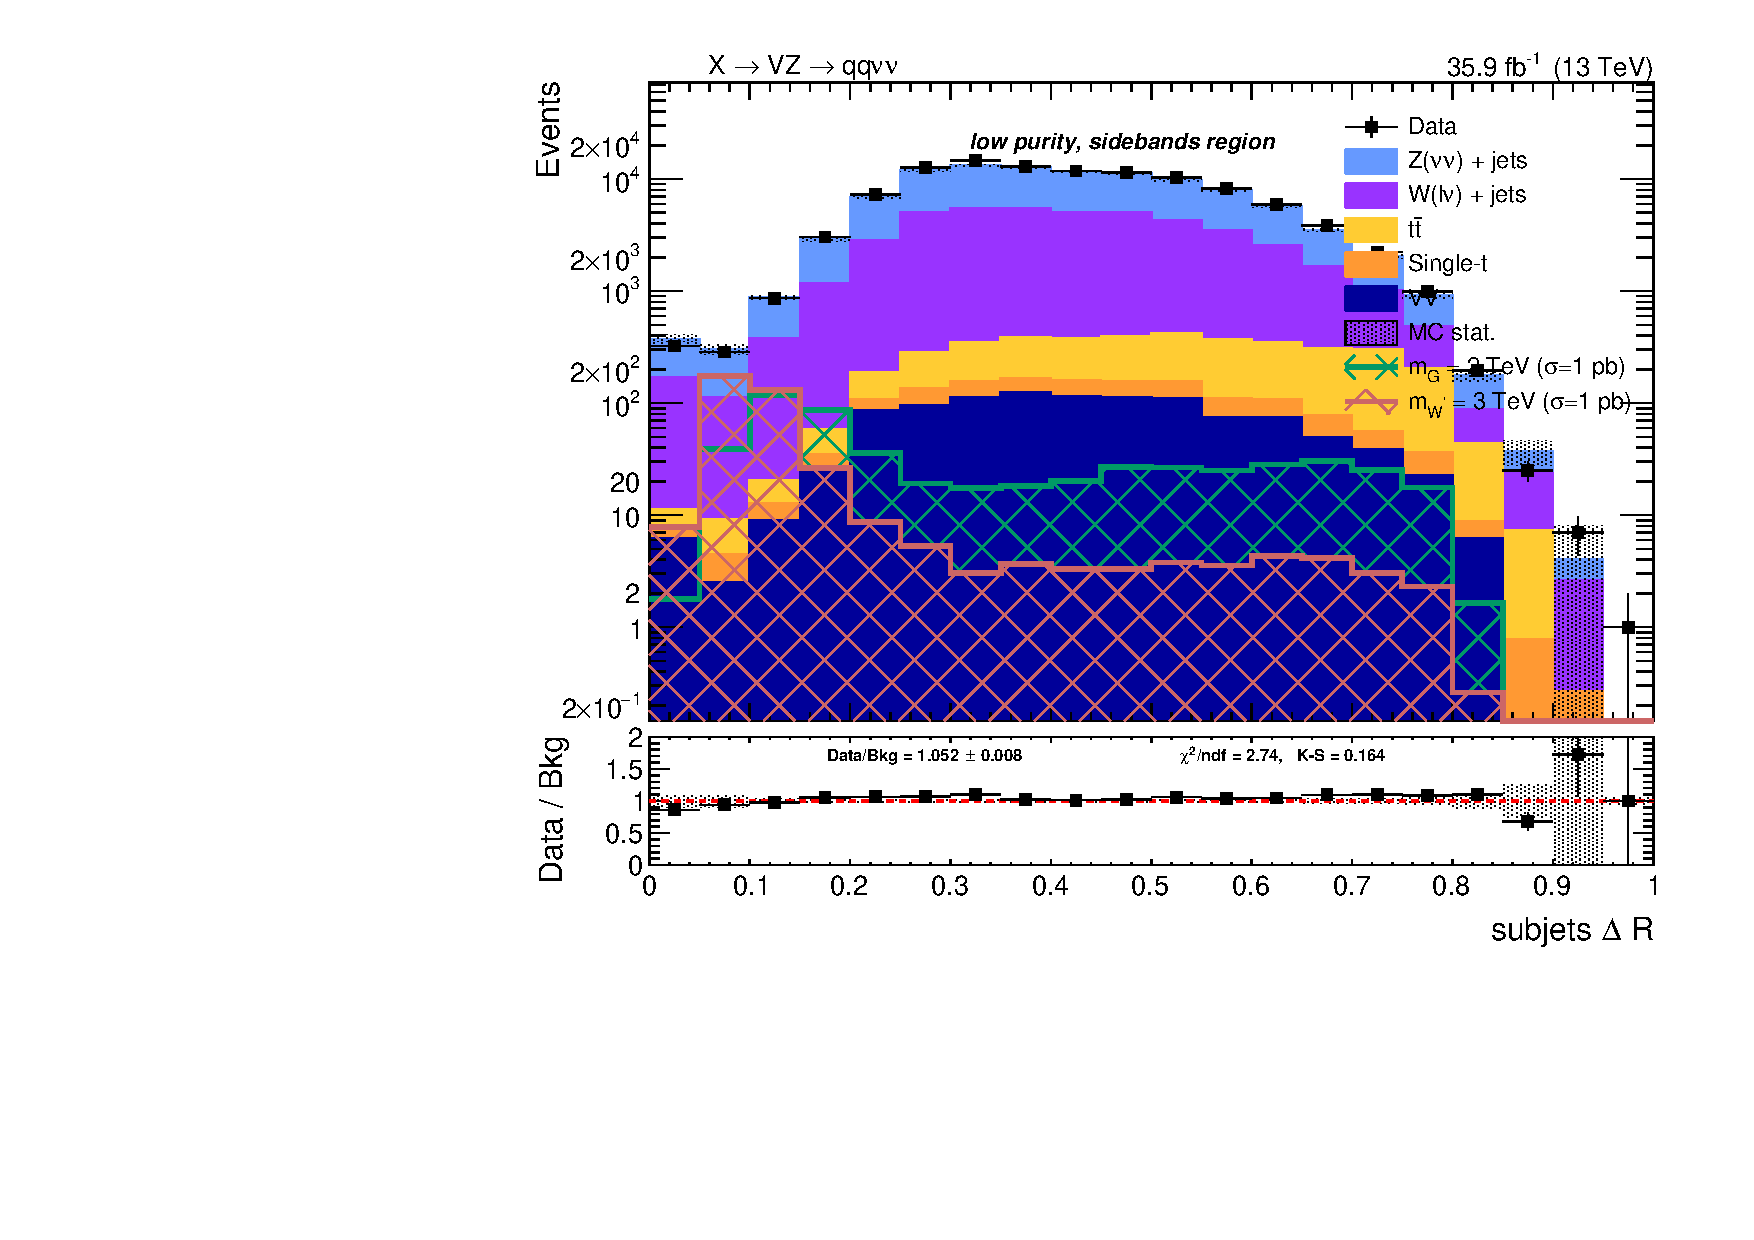
\includegraphics[width=0.495\textwidth]{plots/v9_thesis/XVZnnlpSB/FatJet1_dR.pdf}

    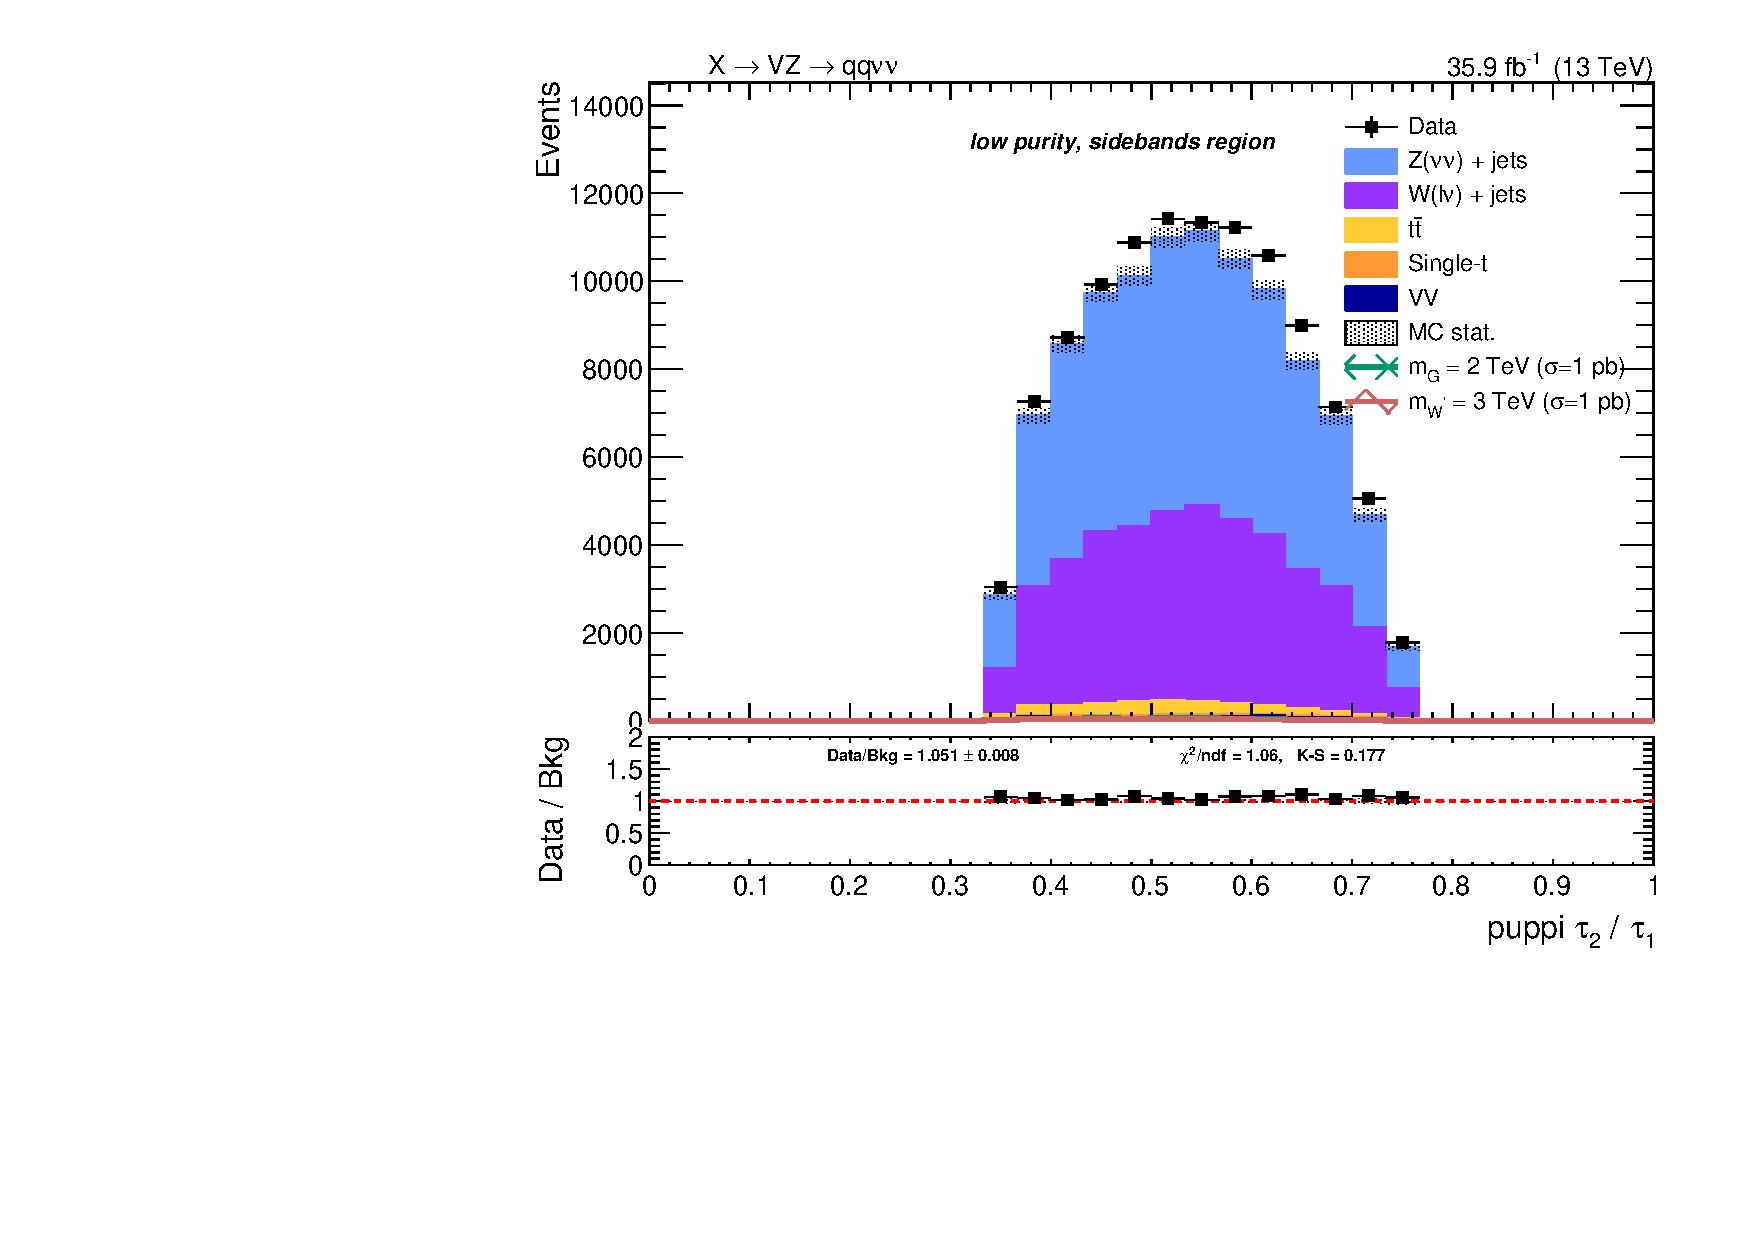
\includegraphics[width=0.495\textwidth]{plots/v9_thesis/XVZnnlpSB/FatJet1_puppiTau21.pdf}
    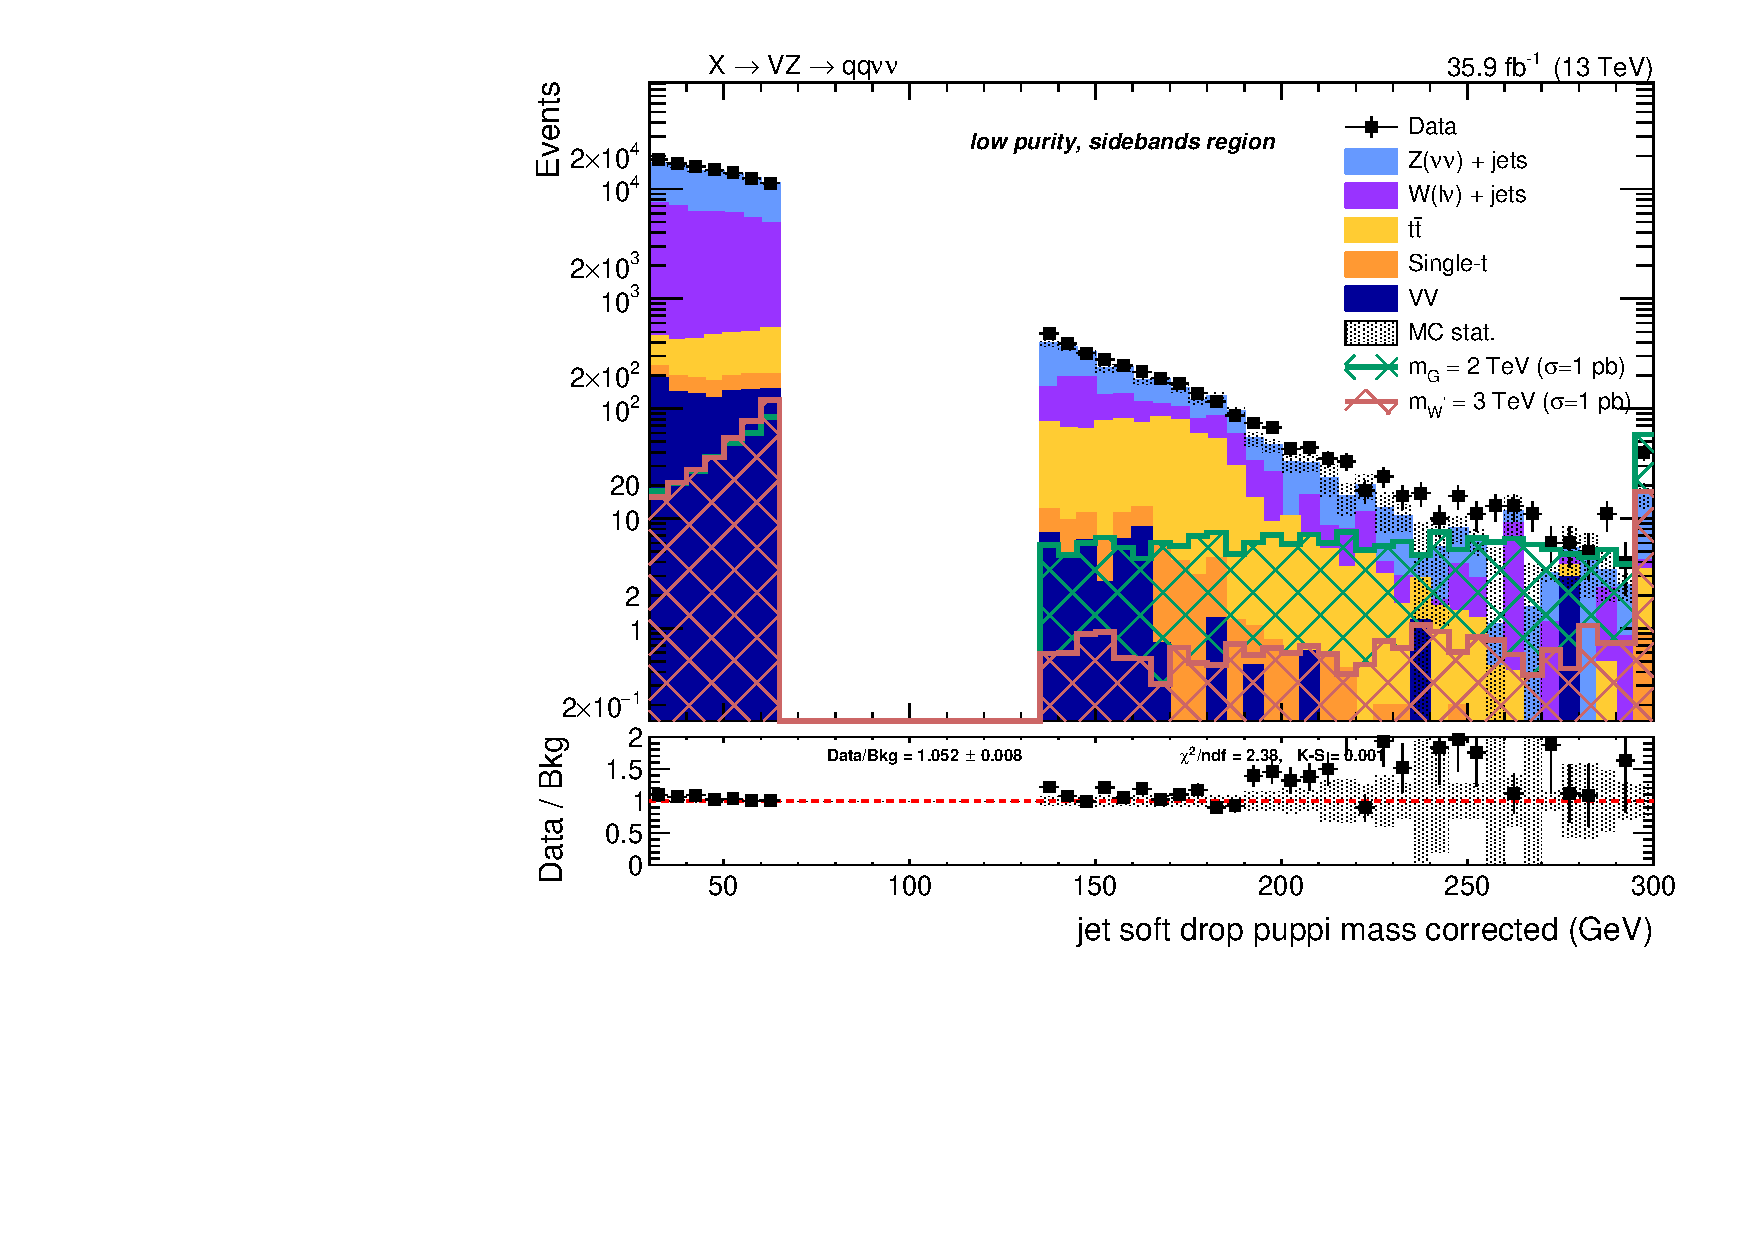
\includegraphics[width=0.495\textwidth]{plots/v9_thesis/XVZnnlpSB/FatJet1_softdropPuppiMassCorr.pdf}

    \caption{Top: number of AK8 jets in the event (left) and \V jet candidate \pt (right). Center: \V jet candidate $\eta$ (left) and angular separation $\Delta R$ between the constituents leading subjets (right). Bottom: \V jet candidate $\tau_{21}$ subjettiness after PUPPI correction (left) and \V jet candidate soft drop PUPPI mass (right). Events are selected with the \emph{low-purity sidebands} selection, and simulated backgrounds are normalized to luminosity.}
%\label{fig:XZhll_N}
  \end{center}
\end{figure}

\clearpage

\begin{figure}[!htb]
  \begin{center}  
    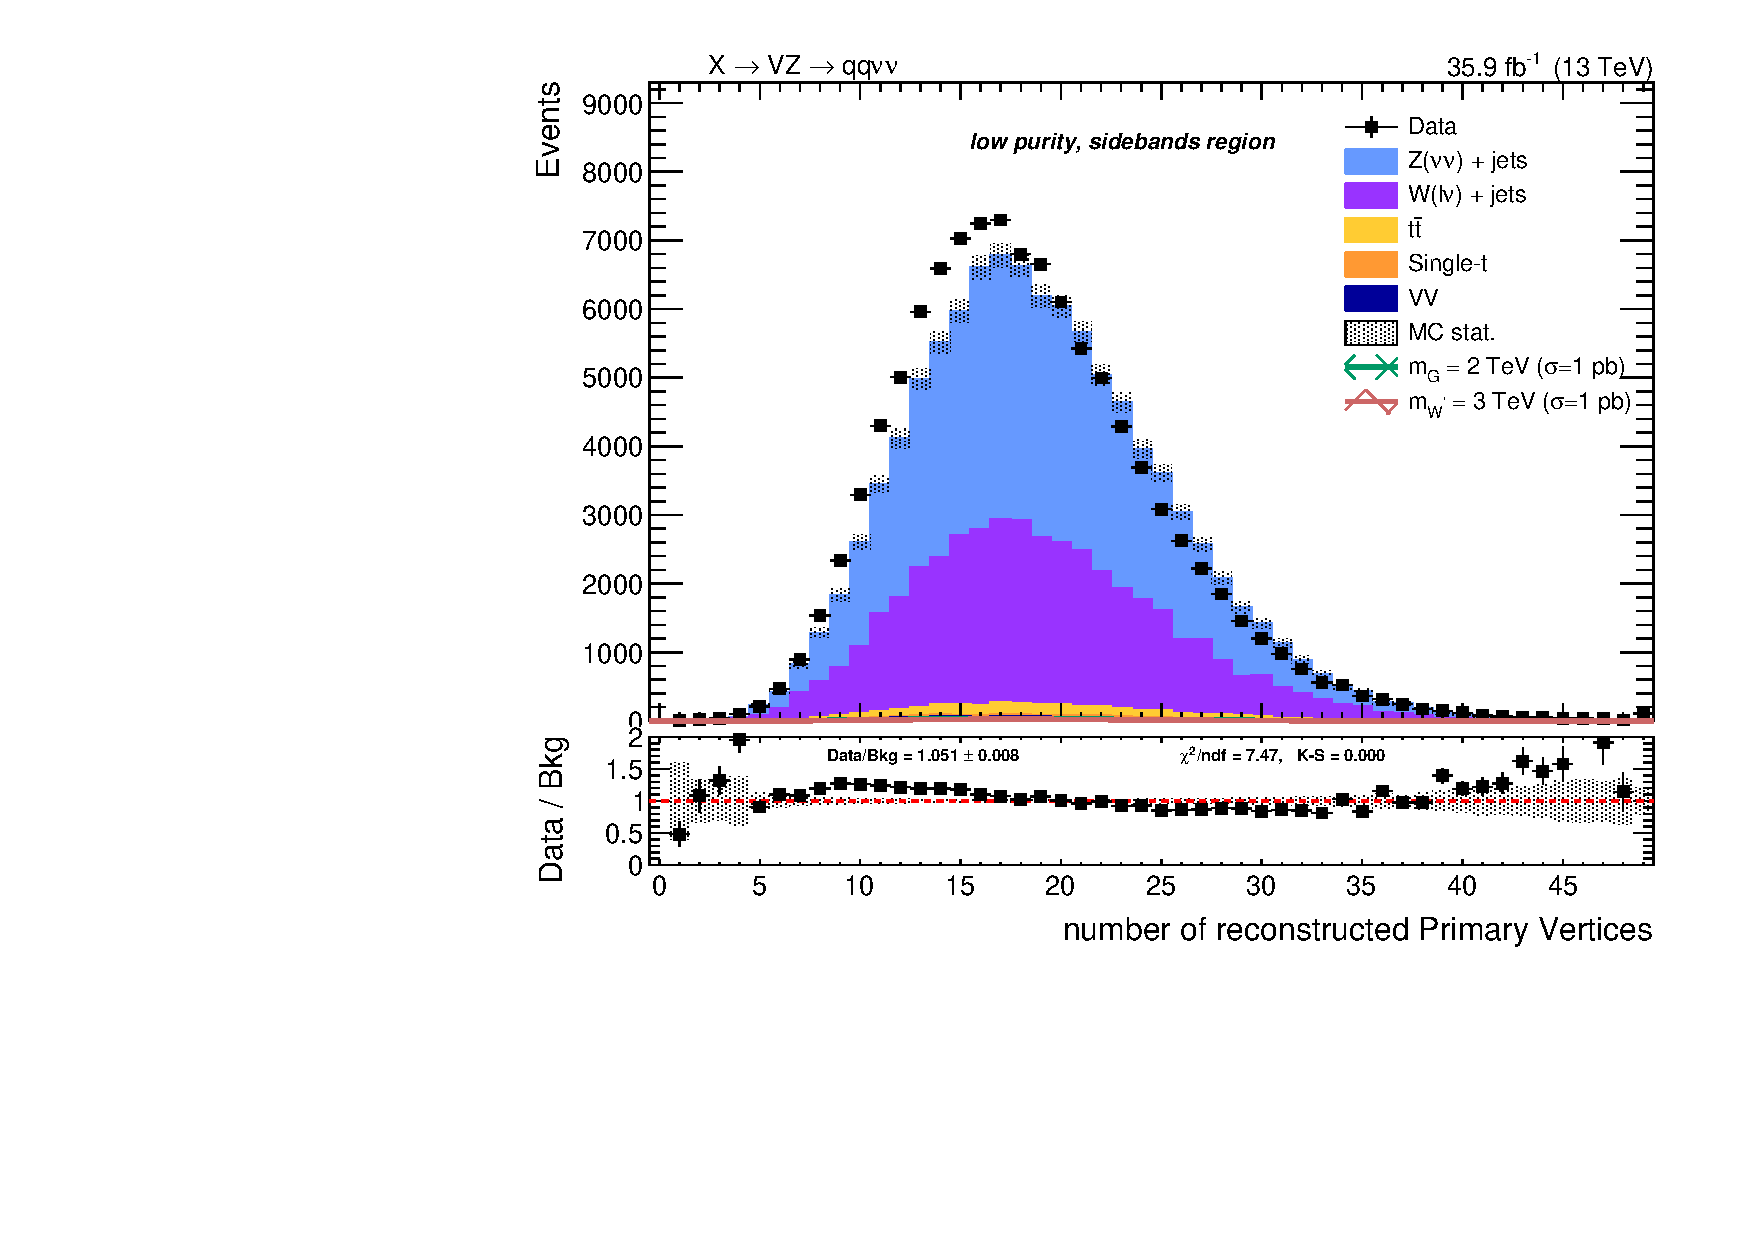
\includegraphics[width=0.495\textwidth]{plots/v9_thesis/XVZnnlpSB/nPV.pdf}
    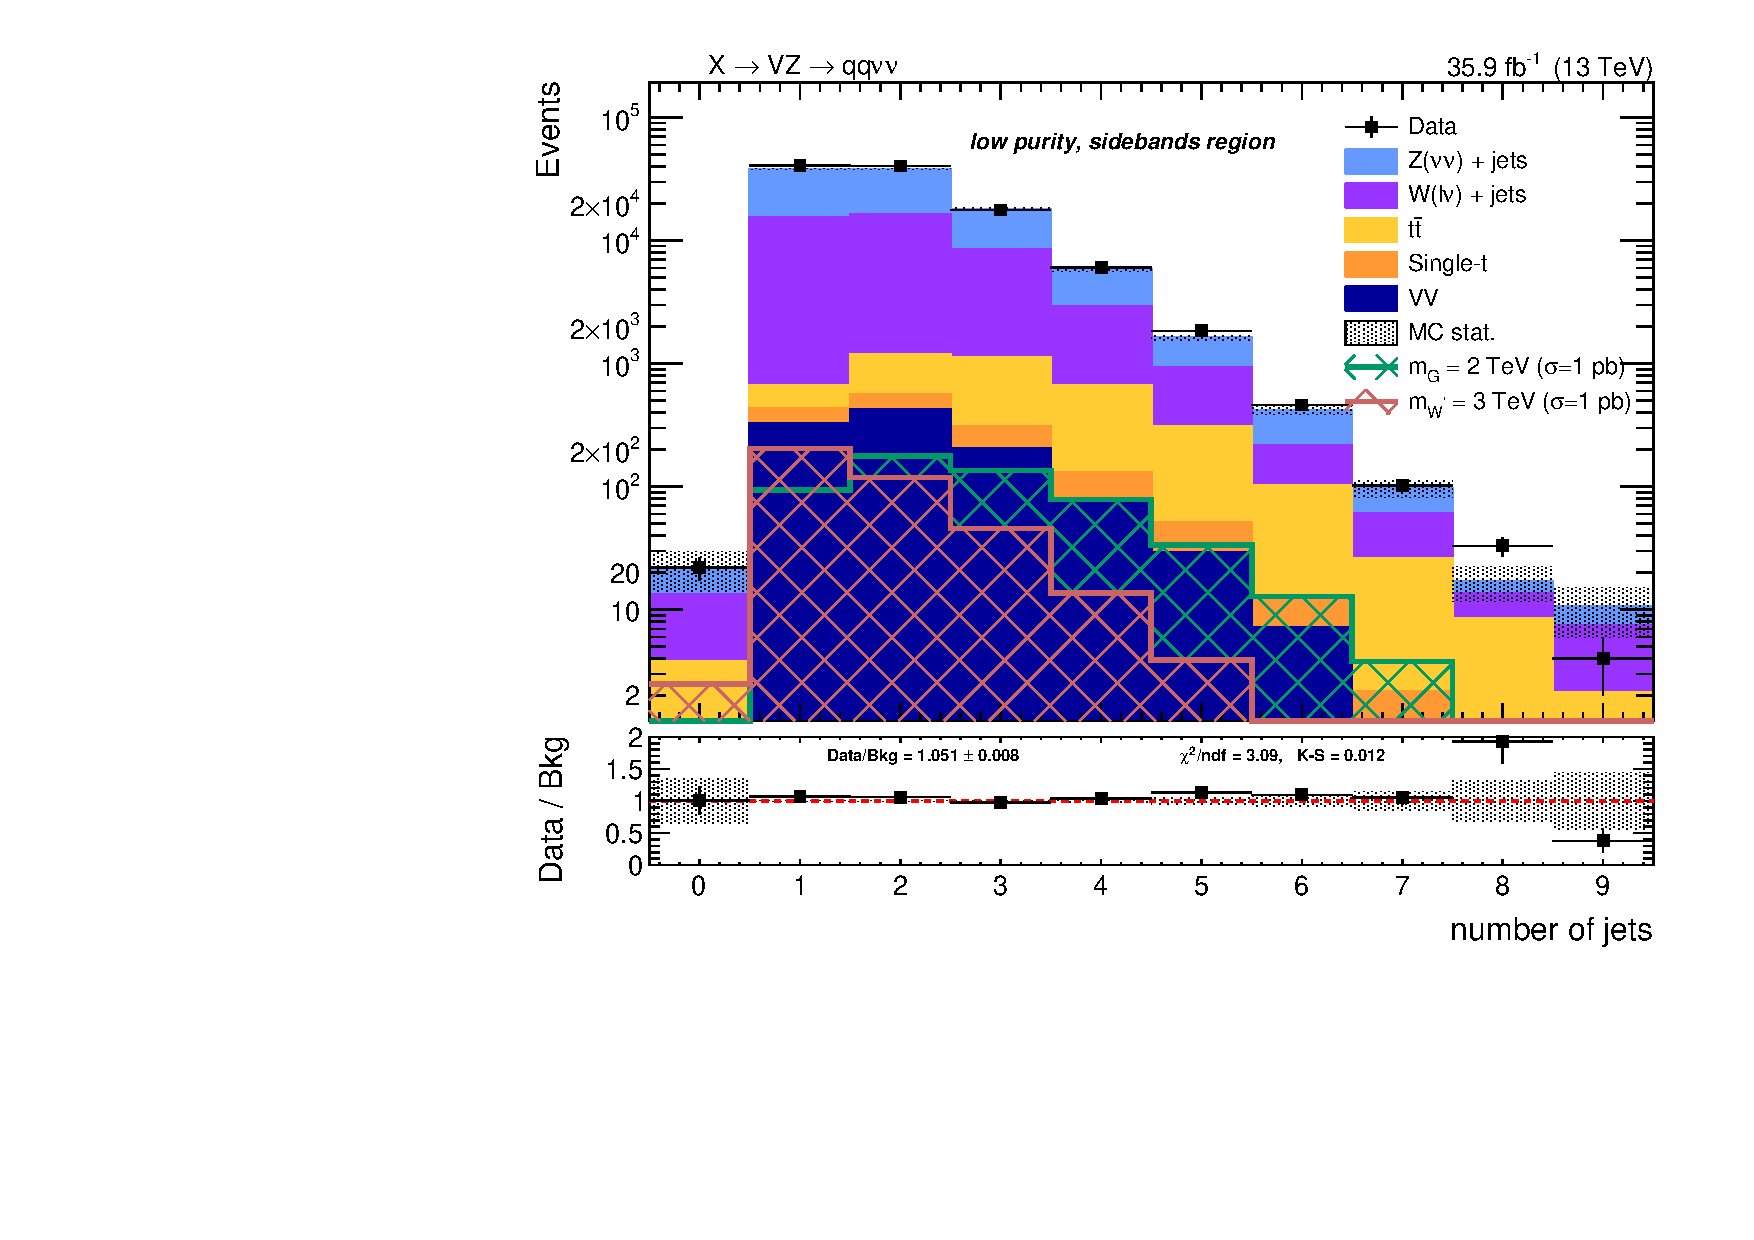
\includegraphics[width=0.495\textwidth]{plots/v9_thesis/XVZnnlpSB/nJets.pdf}

    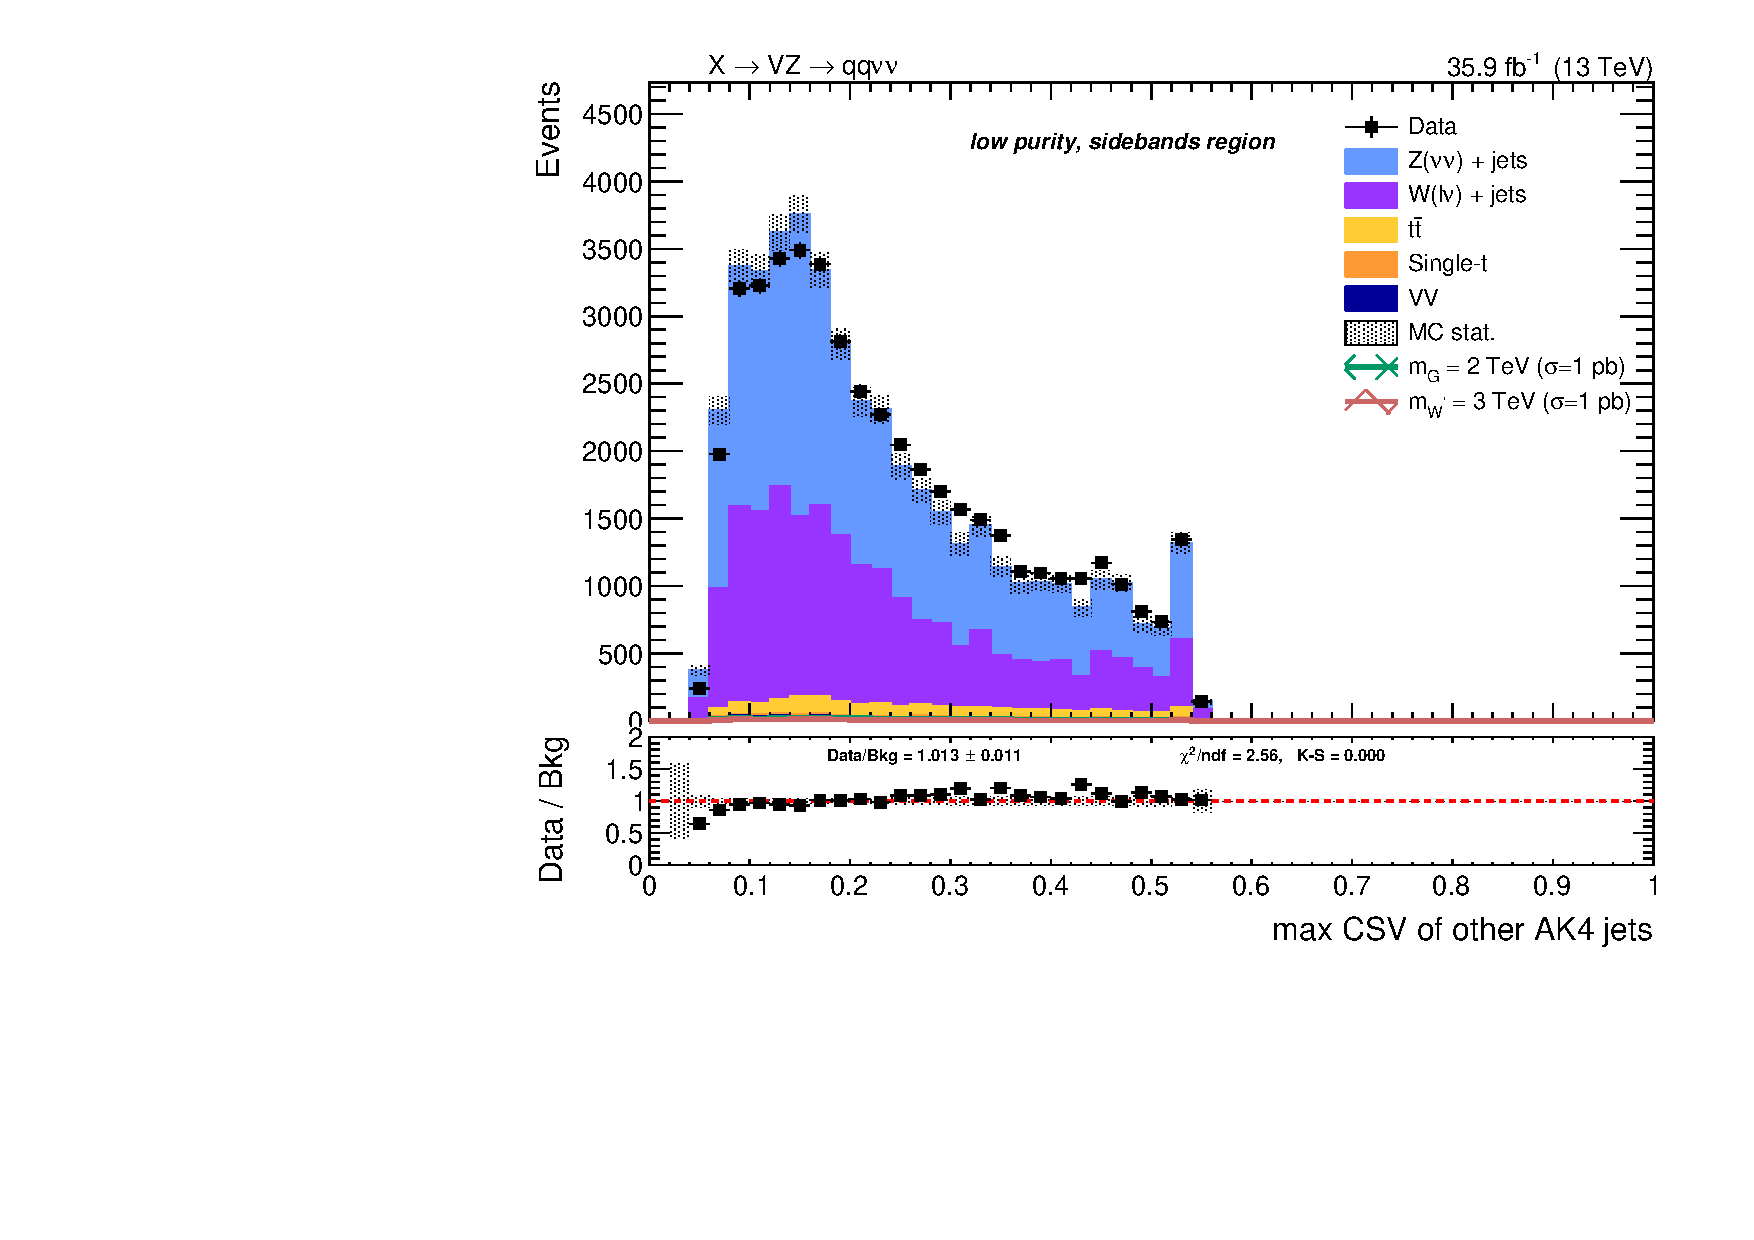
\includegraphics[width=0.495\textwidth]{plots/v9_thesis/XVZnnlpSB/MaxJetBTag.pdf}
    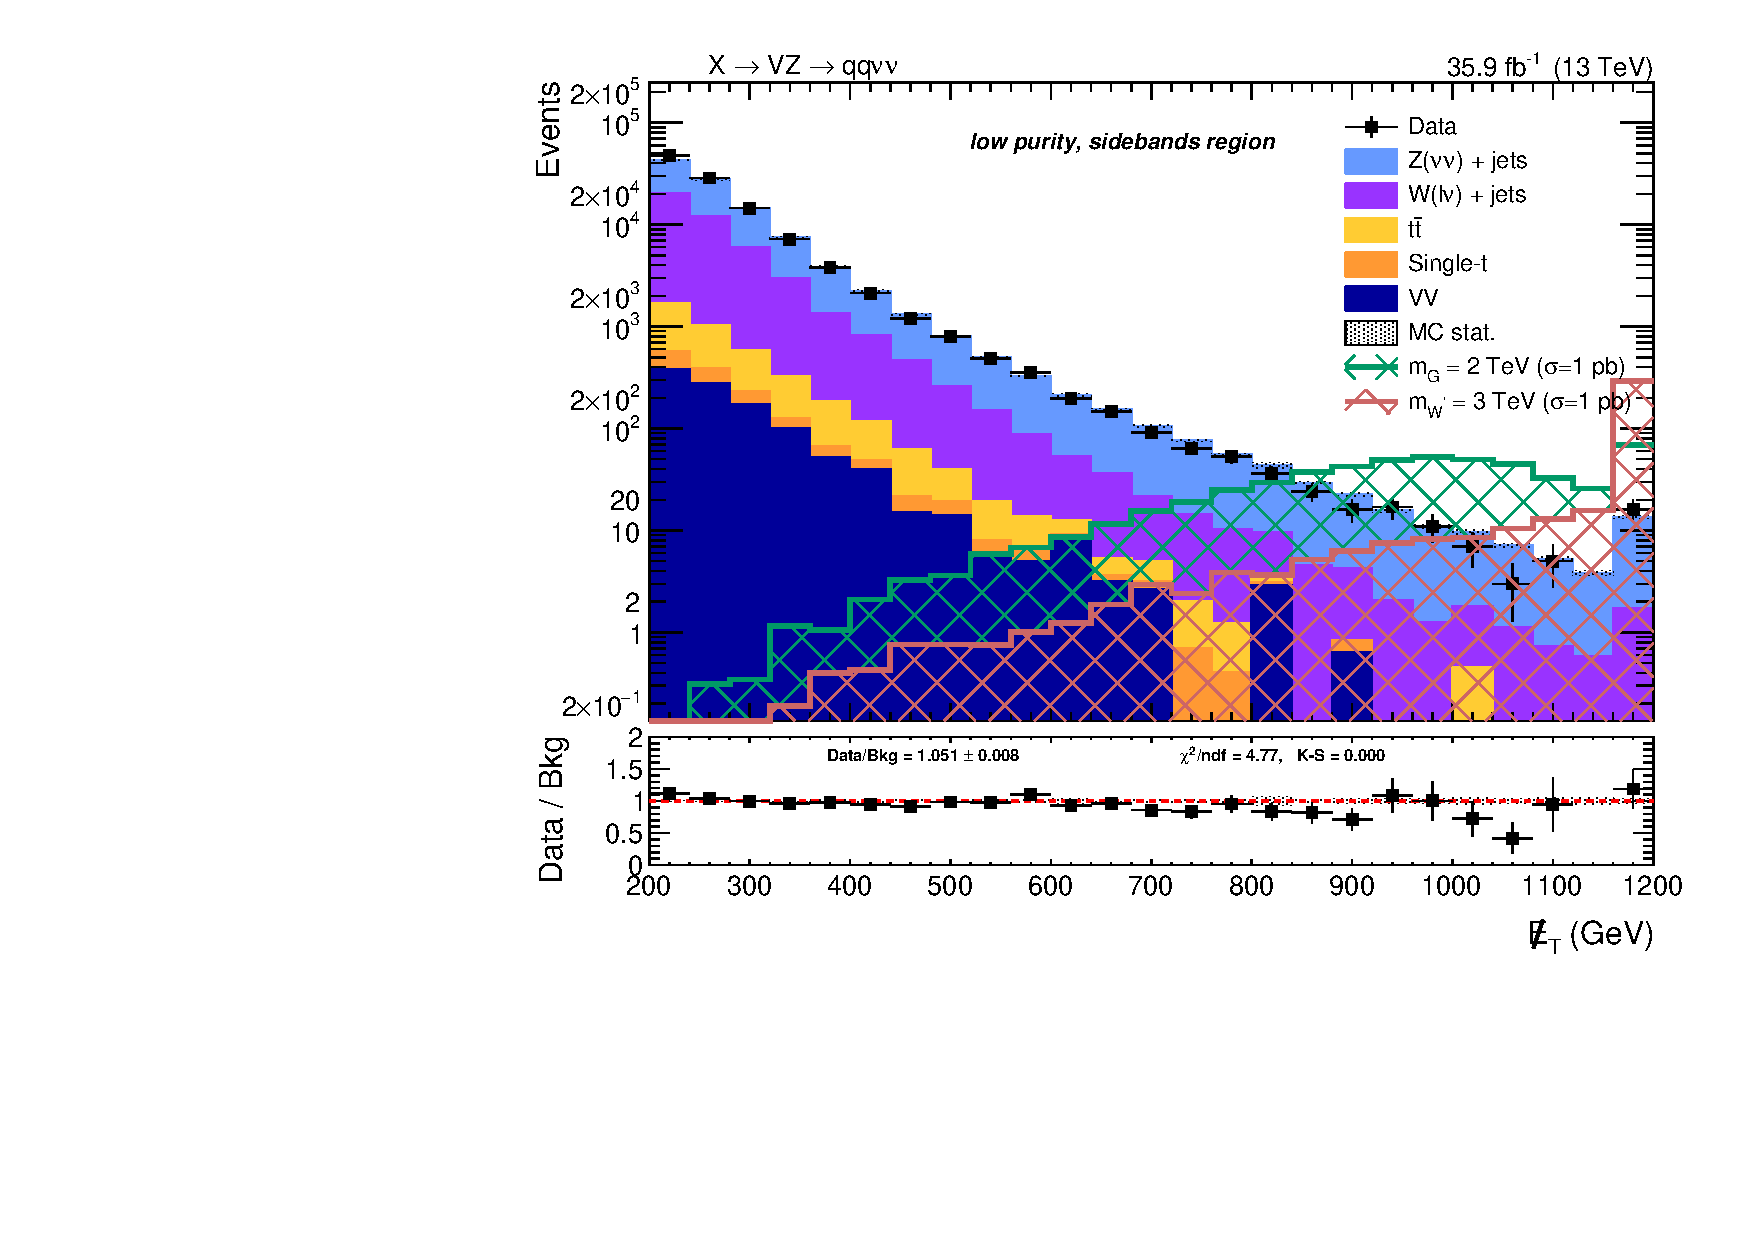
\includegraphics[width=0.495\textwidth]{plots/v9_thesis/XVZnnlpSB/MEt_pt.pdf}

    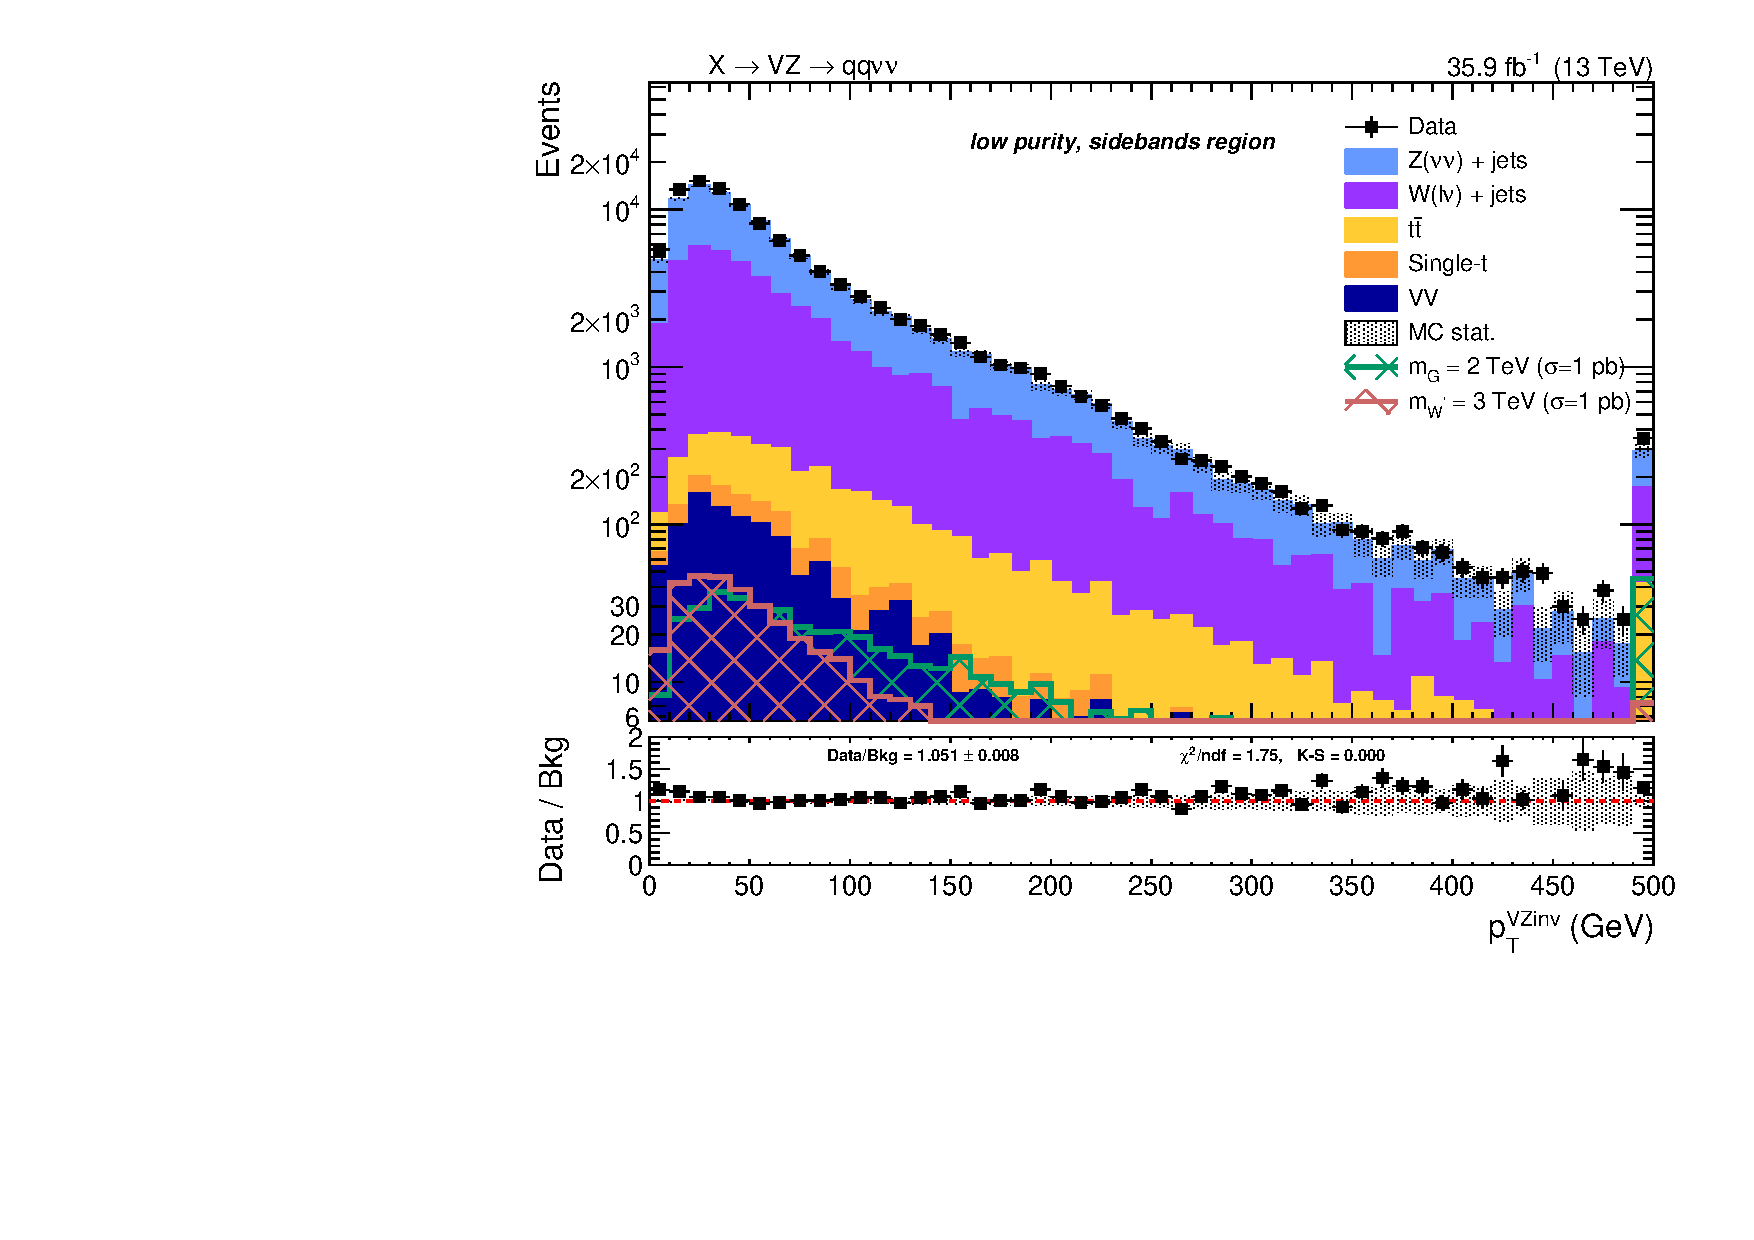
\includegraphics[width=0.495\textwidth]{plots/v9_thesis/XVZnnlpSB/X_pt.pdf}
    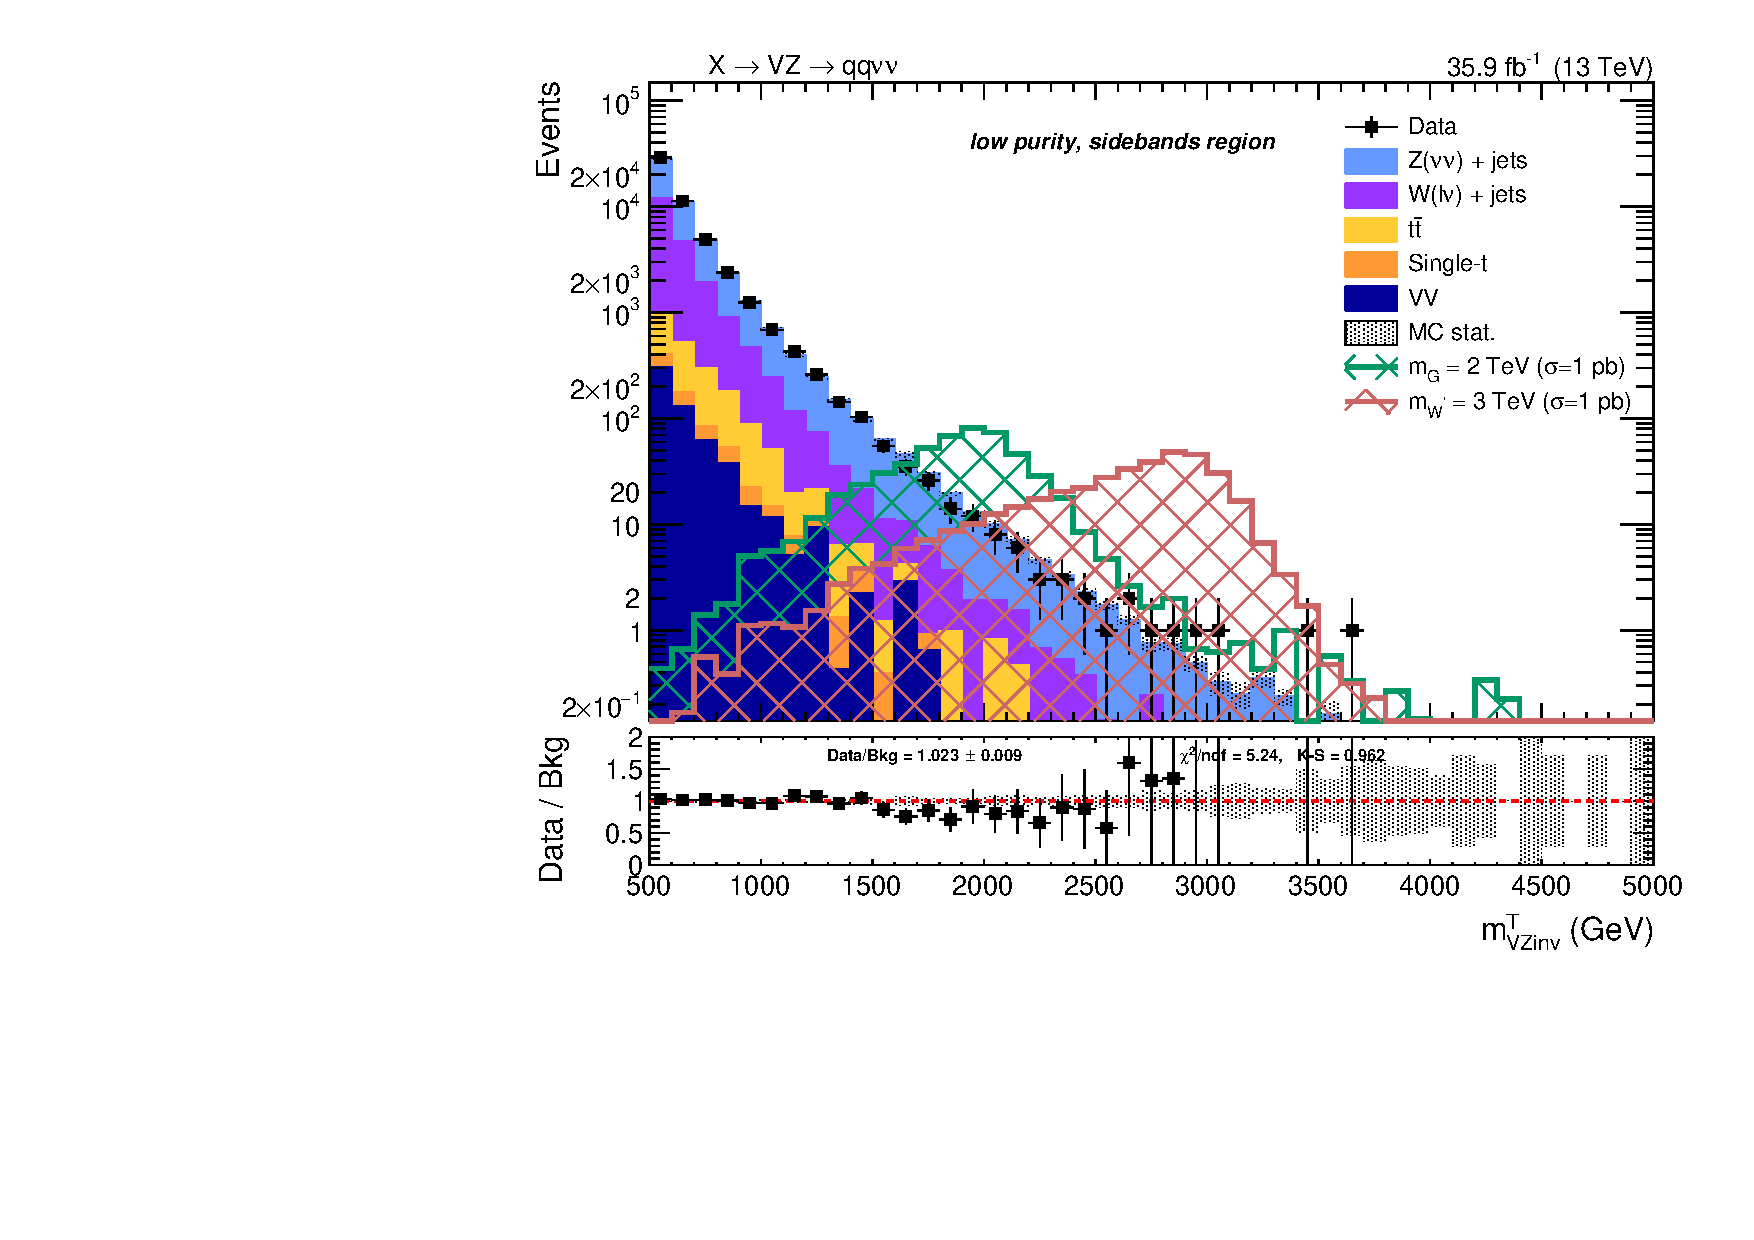
\includegraphics[width=0.495\textwidth]{plots/v9_thesis/XVZnnlpSB/X_tmass.pdf}

    \caption{Top: number of reconstructed primary vertices (left) and number of AK4 jets in the event (right). Center: distribution of the b-tagging multivariate discriminant for the AK4 jets not included in the \V jet cone (left) and \MET distribution (right). Bottom: \pt of the \VZ candidate (left) and transverse mass of the \VZ candidate (right). Events are selected with the \emph{low-purity sidebands} selection, and simulated backgrounds are normalized to luminosity.}
%\label{fig:XZhll_N}
  \end{center}
\end{figure}

\clearpage

%plot scelti
%sideband hp

\begin{figure}[!htb]
  \begin{center}
    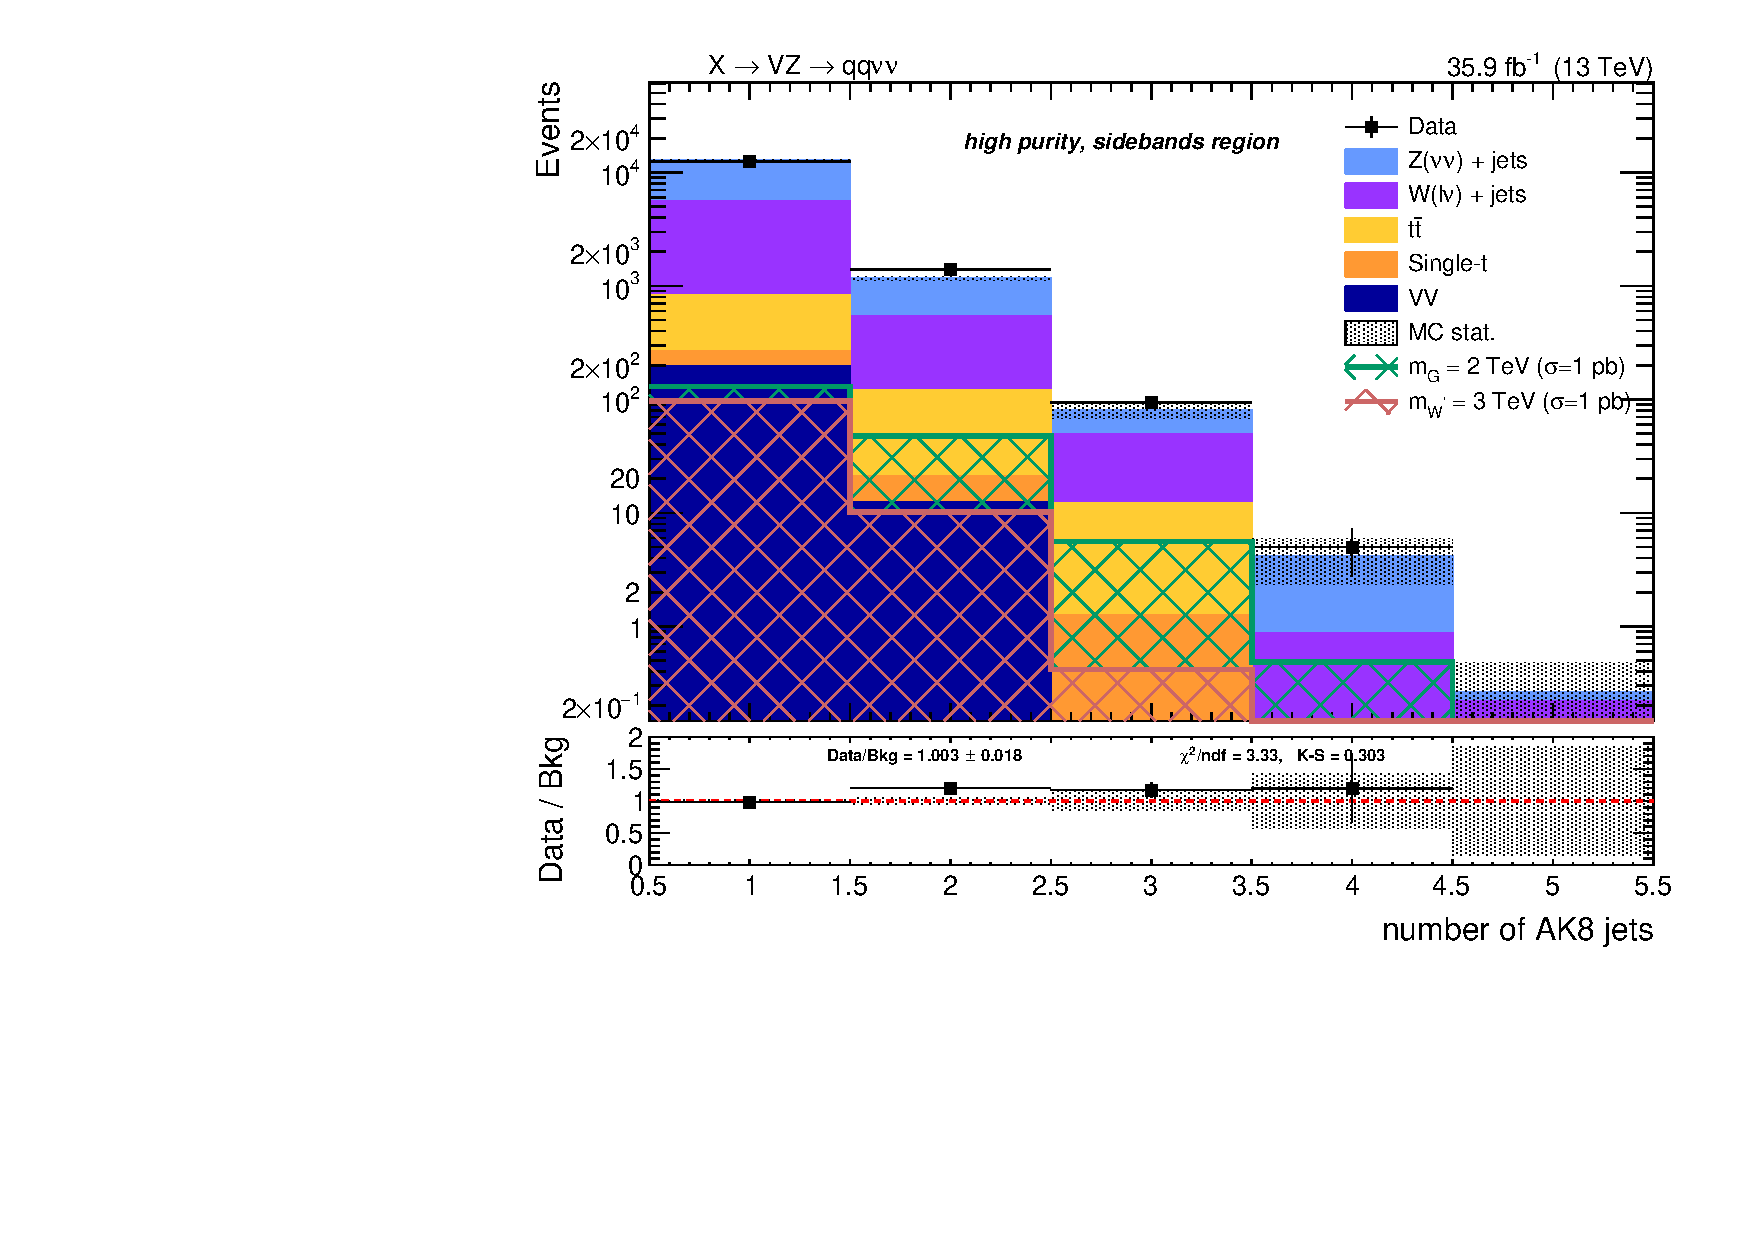
\includegraphics[width=0.495\textwidth]{plots/v9_thesis/XVZnnhpSB/nFatJets.pdf}  
    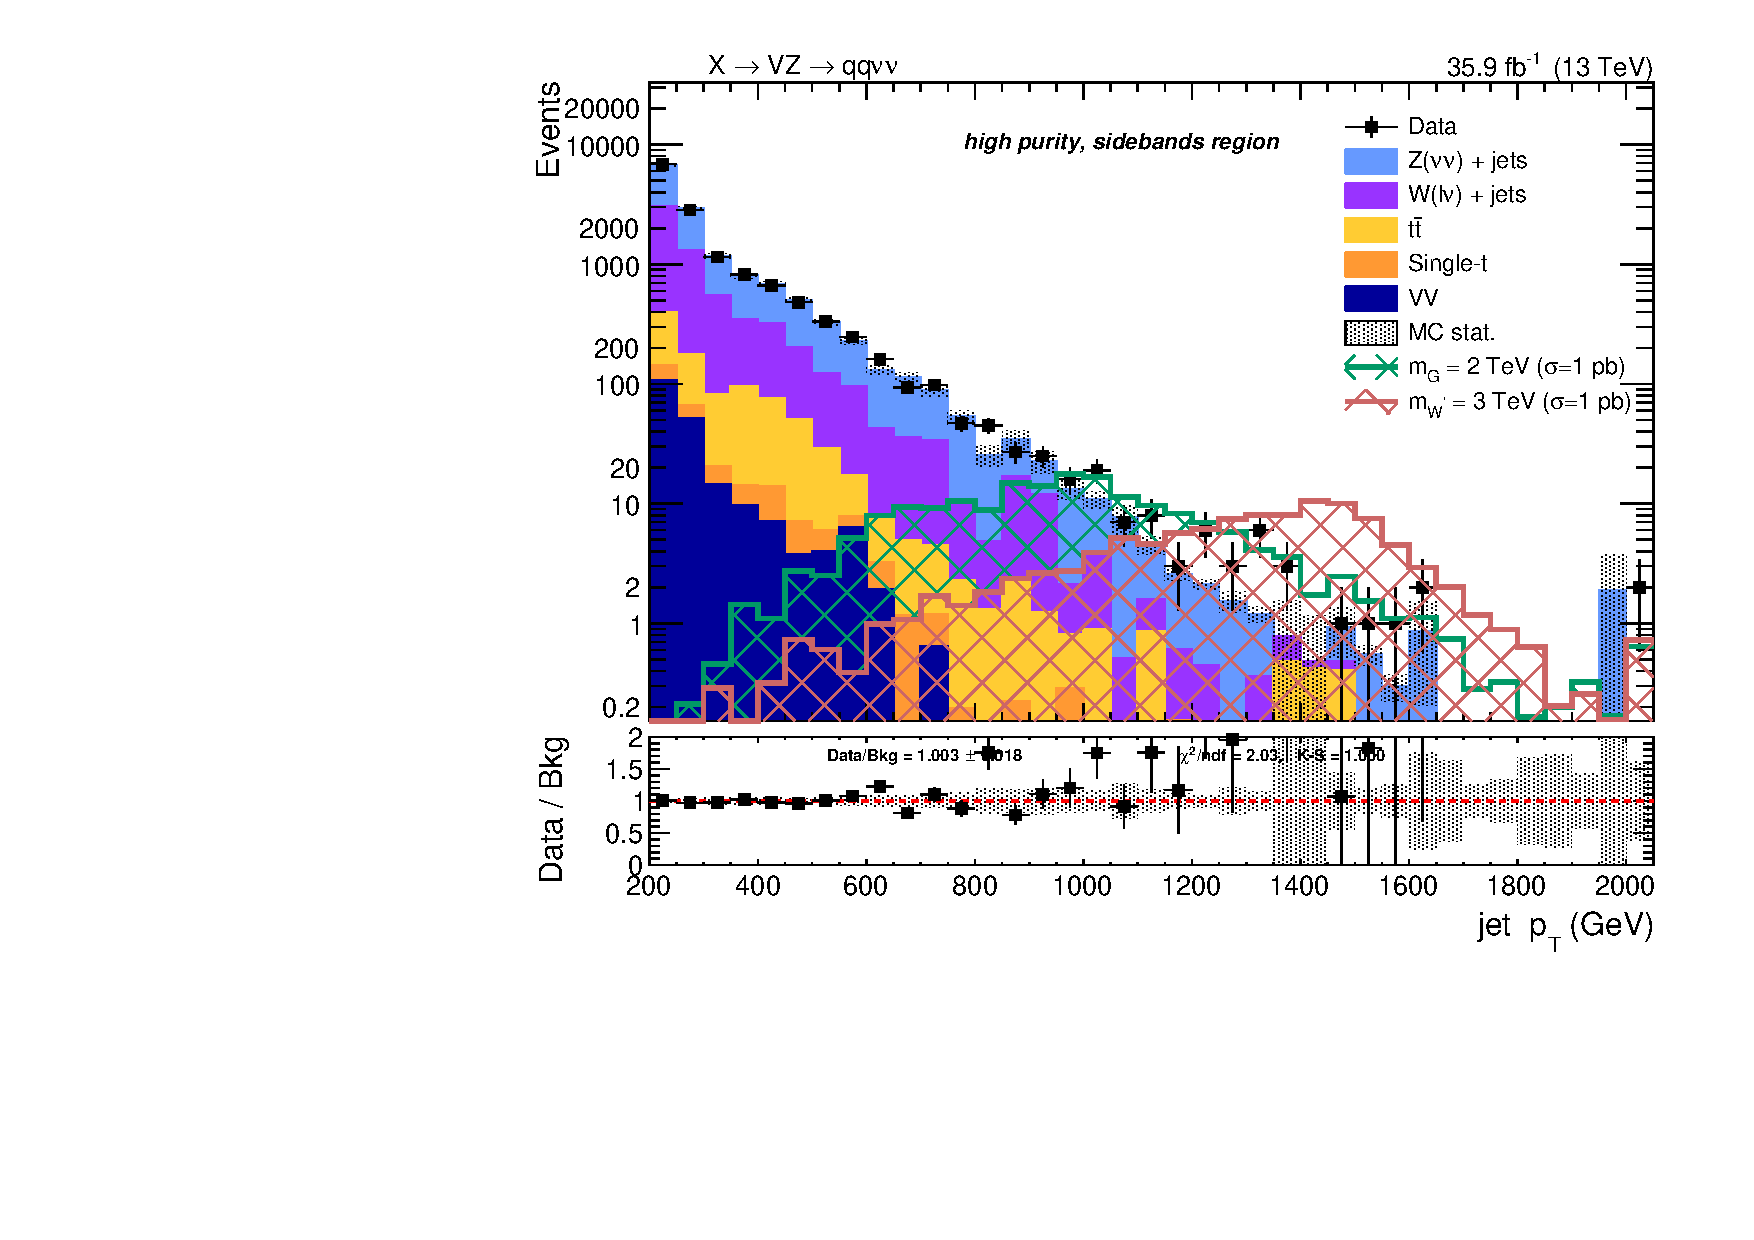
\includegraphics[width=0.495\textwidth]{plots/v9_thesis/XVZnnhpSB/FatJet1_pt.pdf}
    
    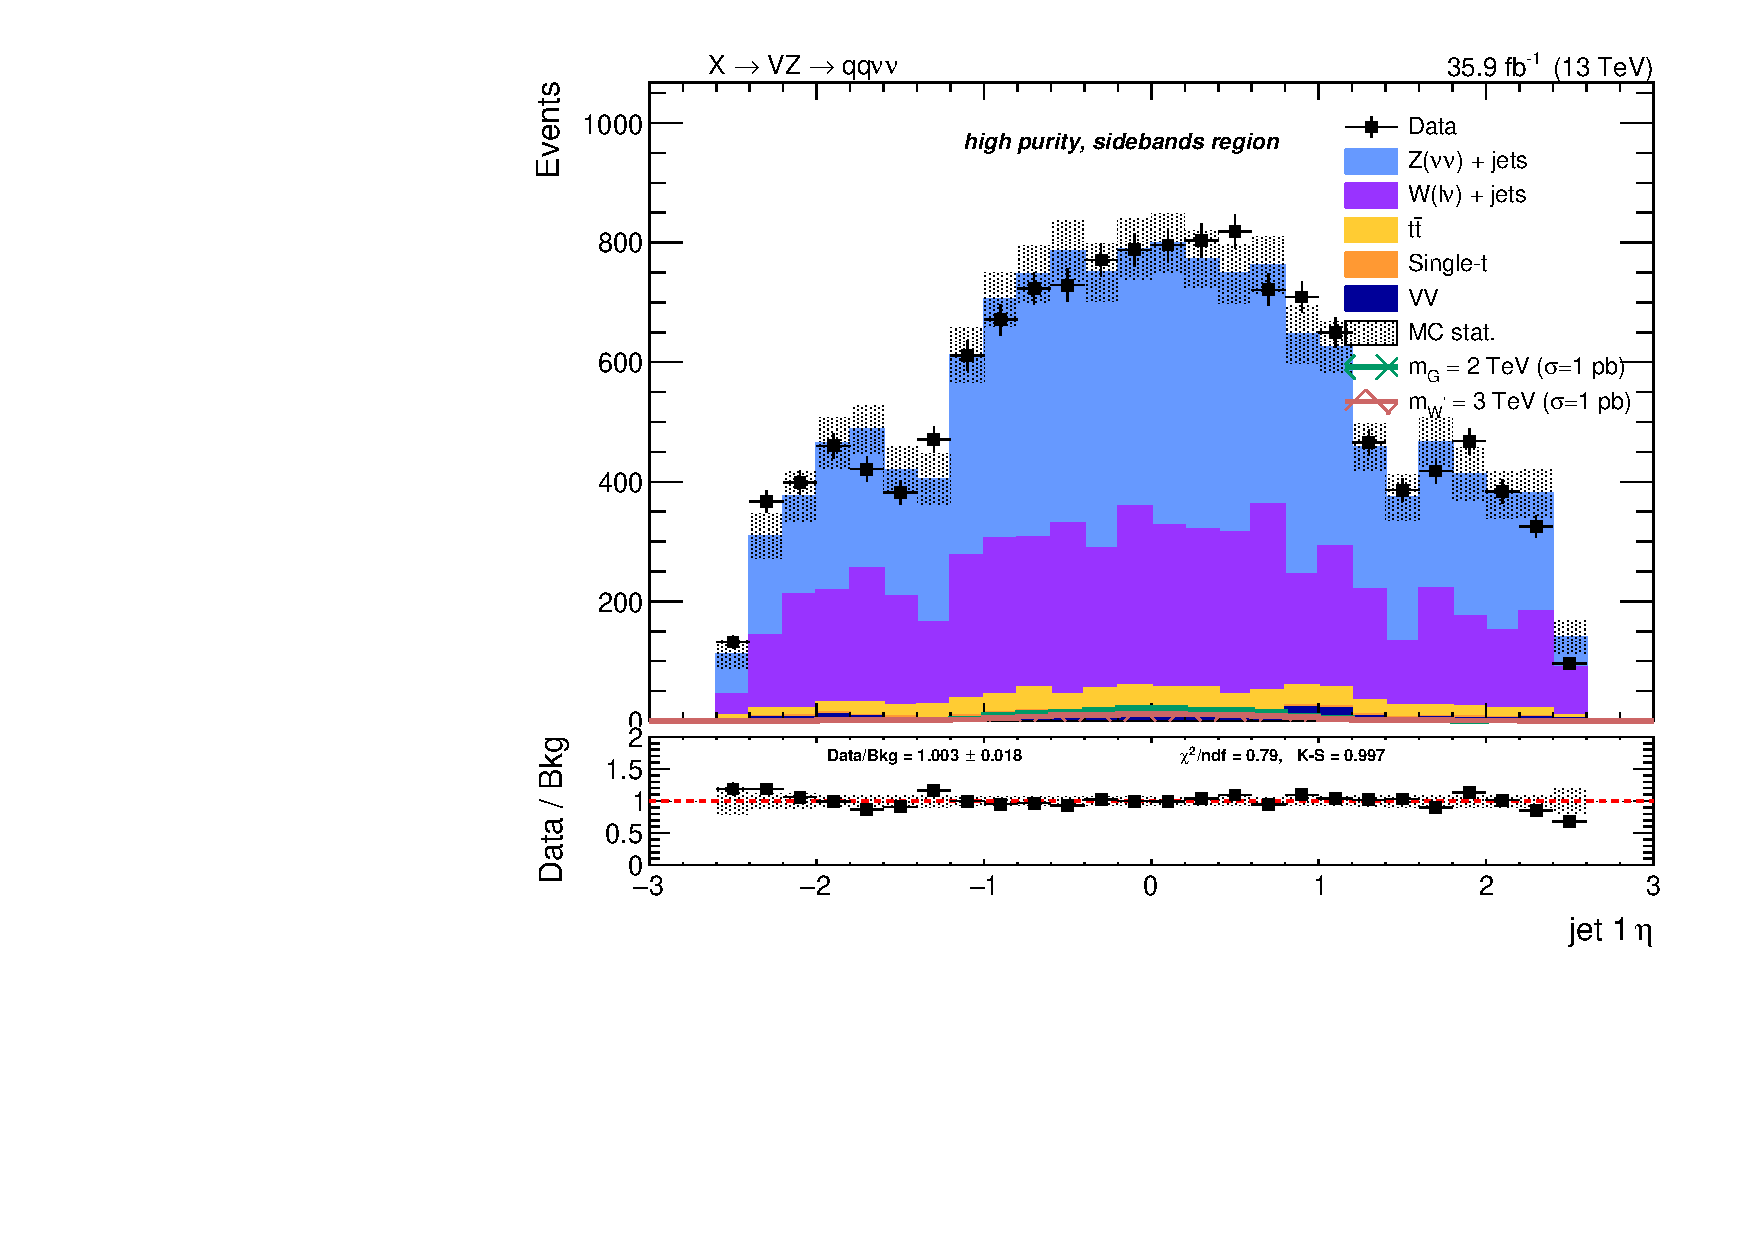
\includegraphics[width=0.495\textwidth]{plots/v9_thesis/XVZnnhpSB/FatJet1_eta.pdf}
    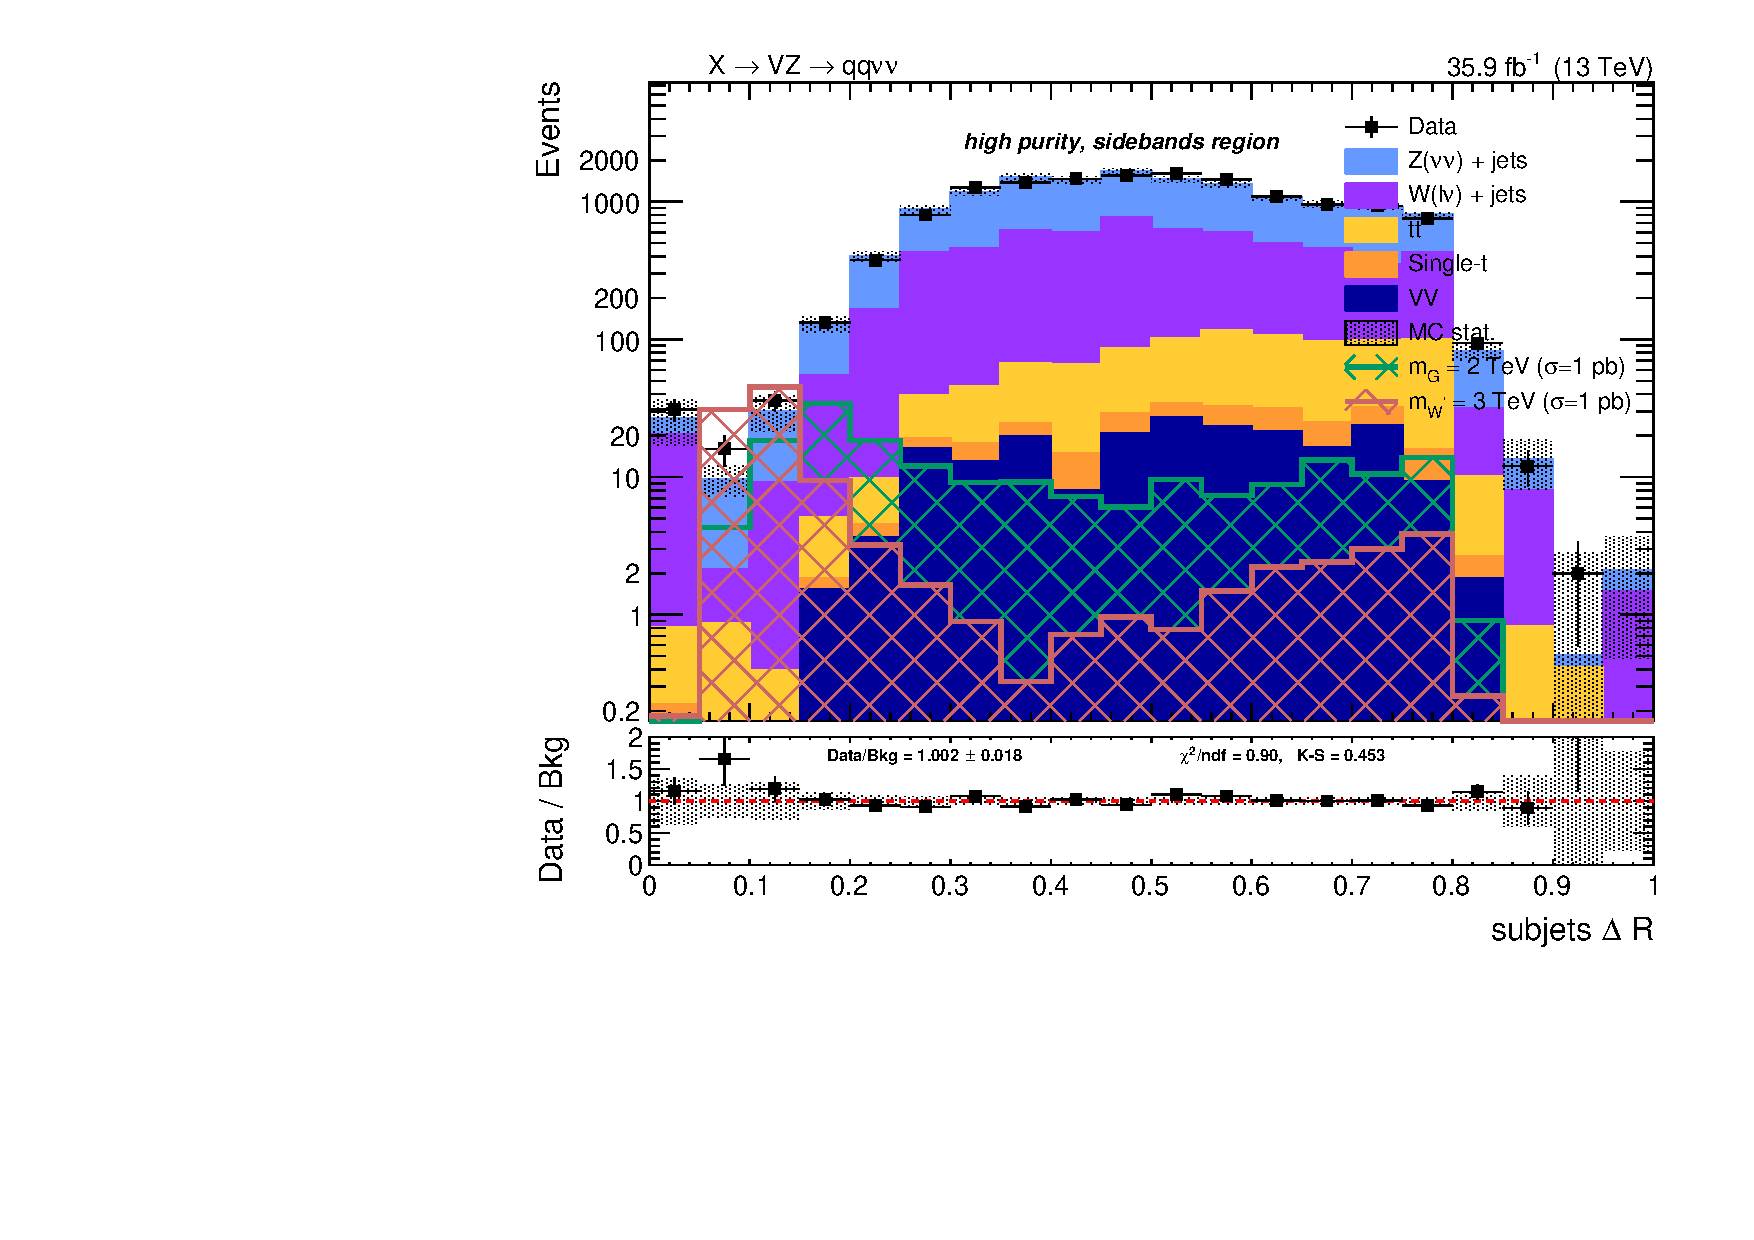
\includegraphics[width=0.495\textwidth]{plots/v9_thesis/XVZnnhpSB/FatJet1_dR.pdf}

    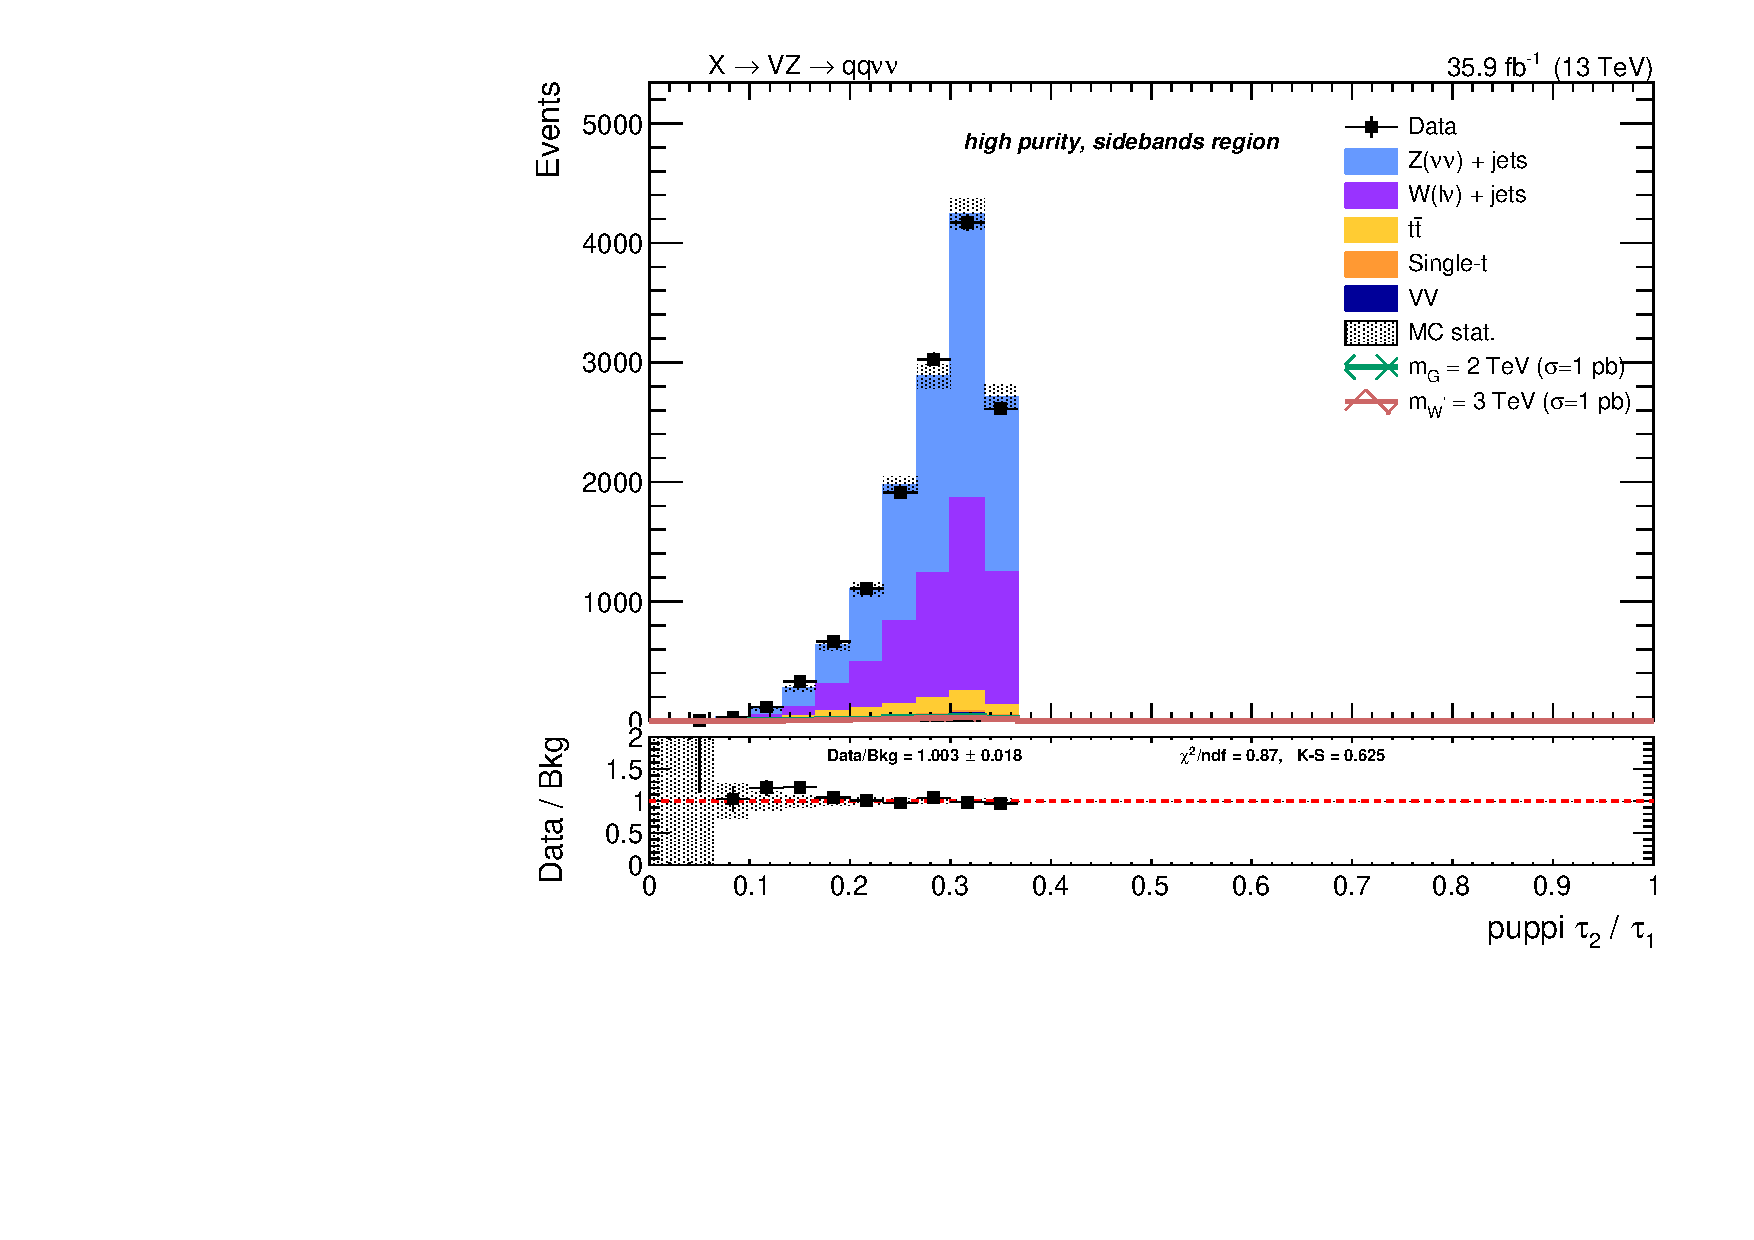
\includegraphics[width=0.495\textwidth]{plots/v9_thesis/XVZnnhpSB/FatJet1_puppiTau21.pdf}
    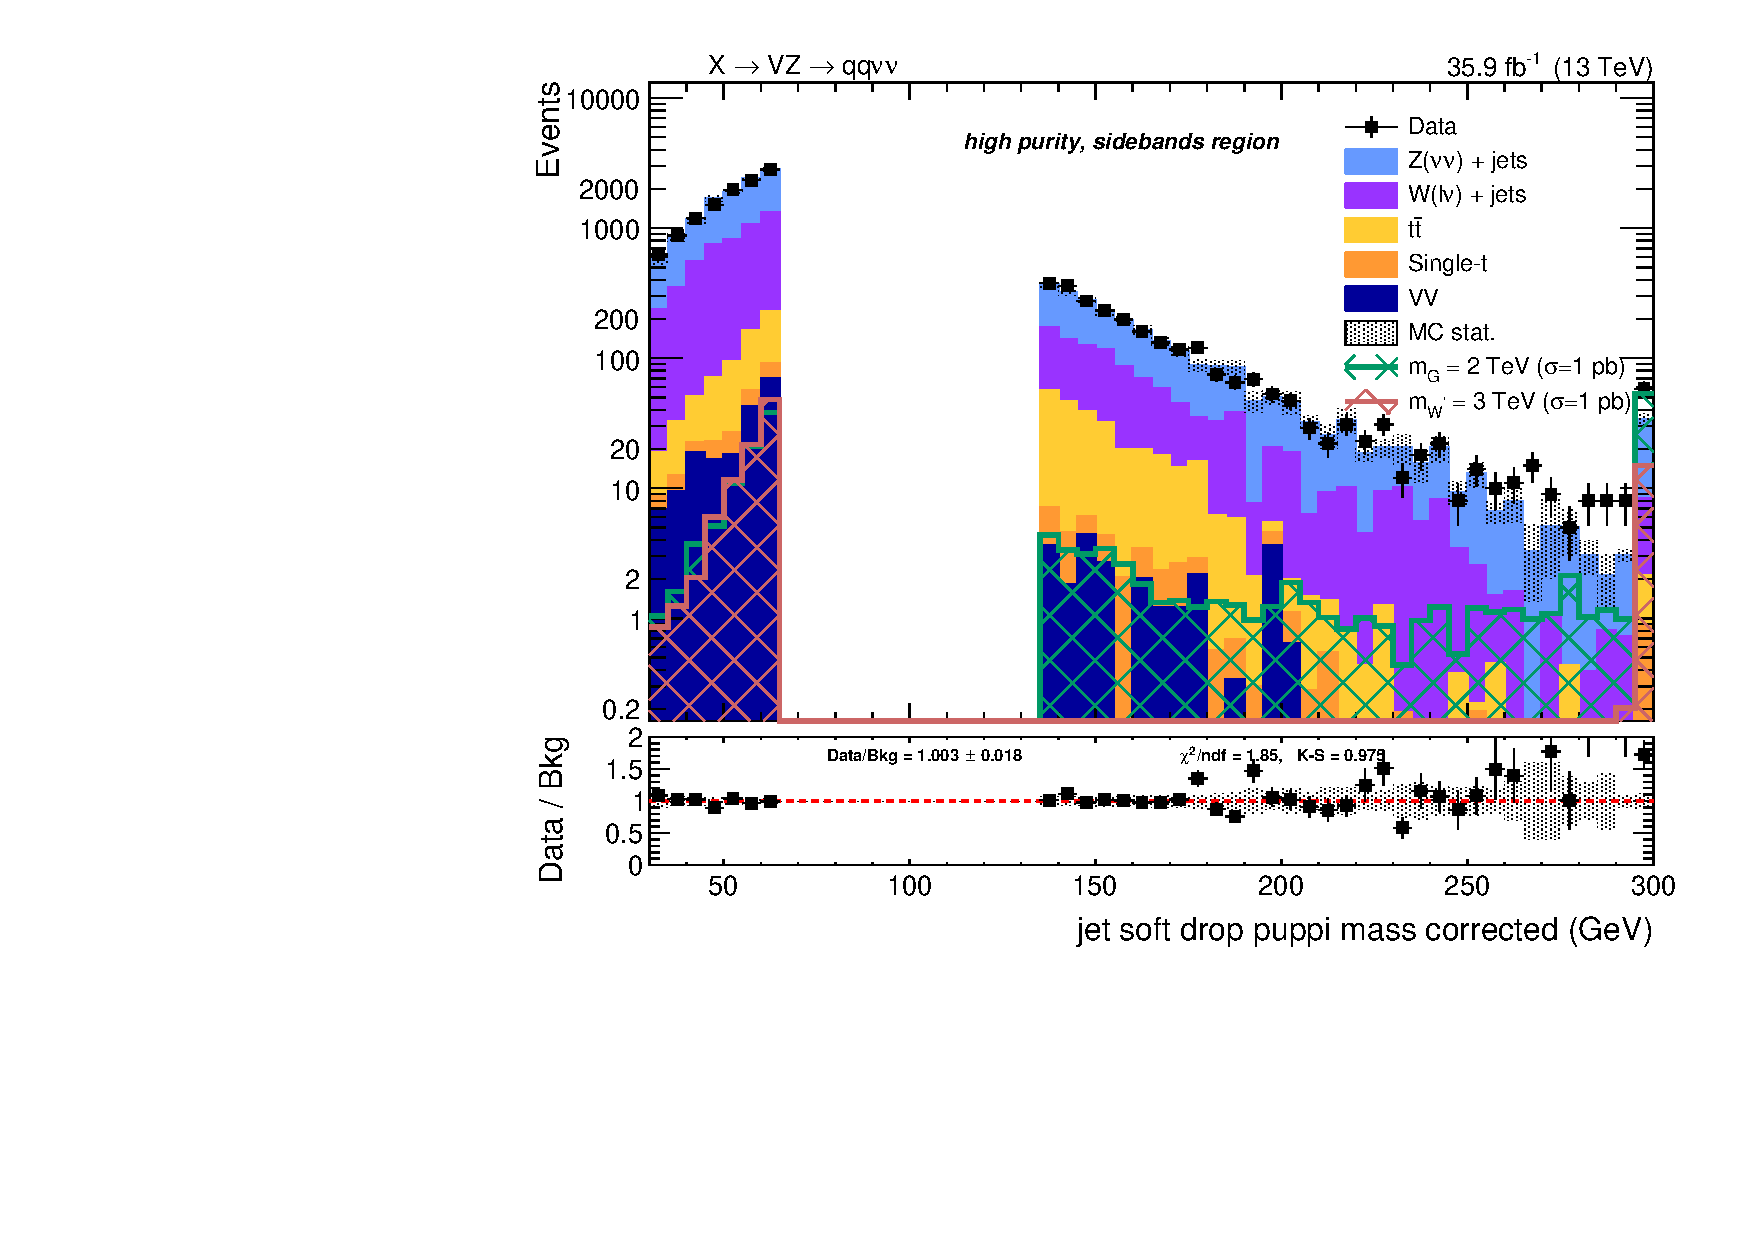
\includegraphics[width=0.495\textwidth]{plots/v9_thesis/XVZnnhpSB/FatJet1_softdropPuppiMassCorr.pdf}

    \caption{Top: number of AK8 jets in the event (left) and \V jet candidate \pt (right). Center: \V jet candidate $\eta$ (left) and angular separation $\Delta R$ between the constituents leading subjets (right). Bottom: \V jet candidate $\tau_{21}$ subjettiness after PUPPI correction (left) and \V jet candidate soft drop PUPPI mass (right). Events are selected with the \emph{high-purity sidebands} selection, and simulated backgrounds are normalized to luminosity.}
%\label{fig:XZhll_N}
  \end{center}
\end{figure}

\clearpage

\begin{figure}[!htb]
  \begin{center}  
    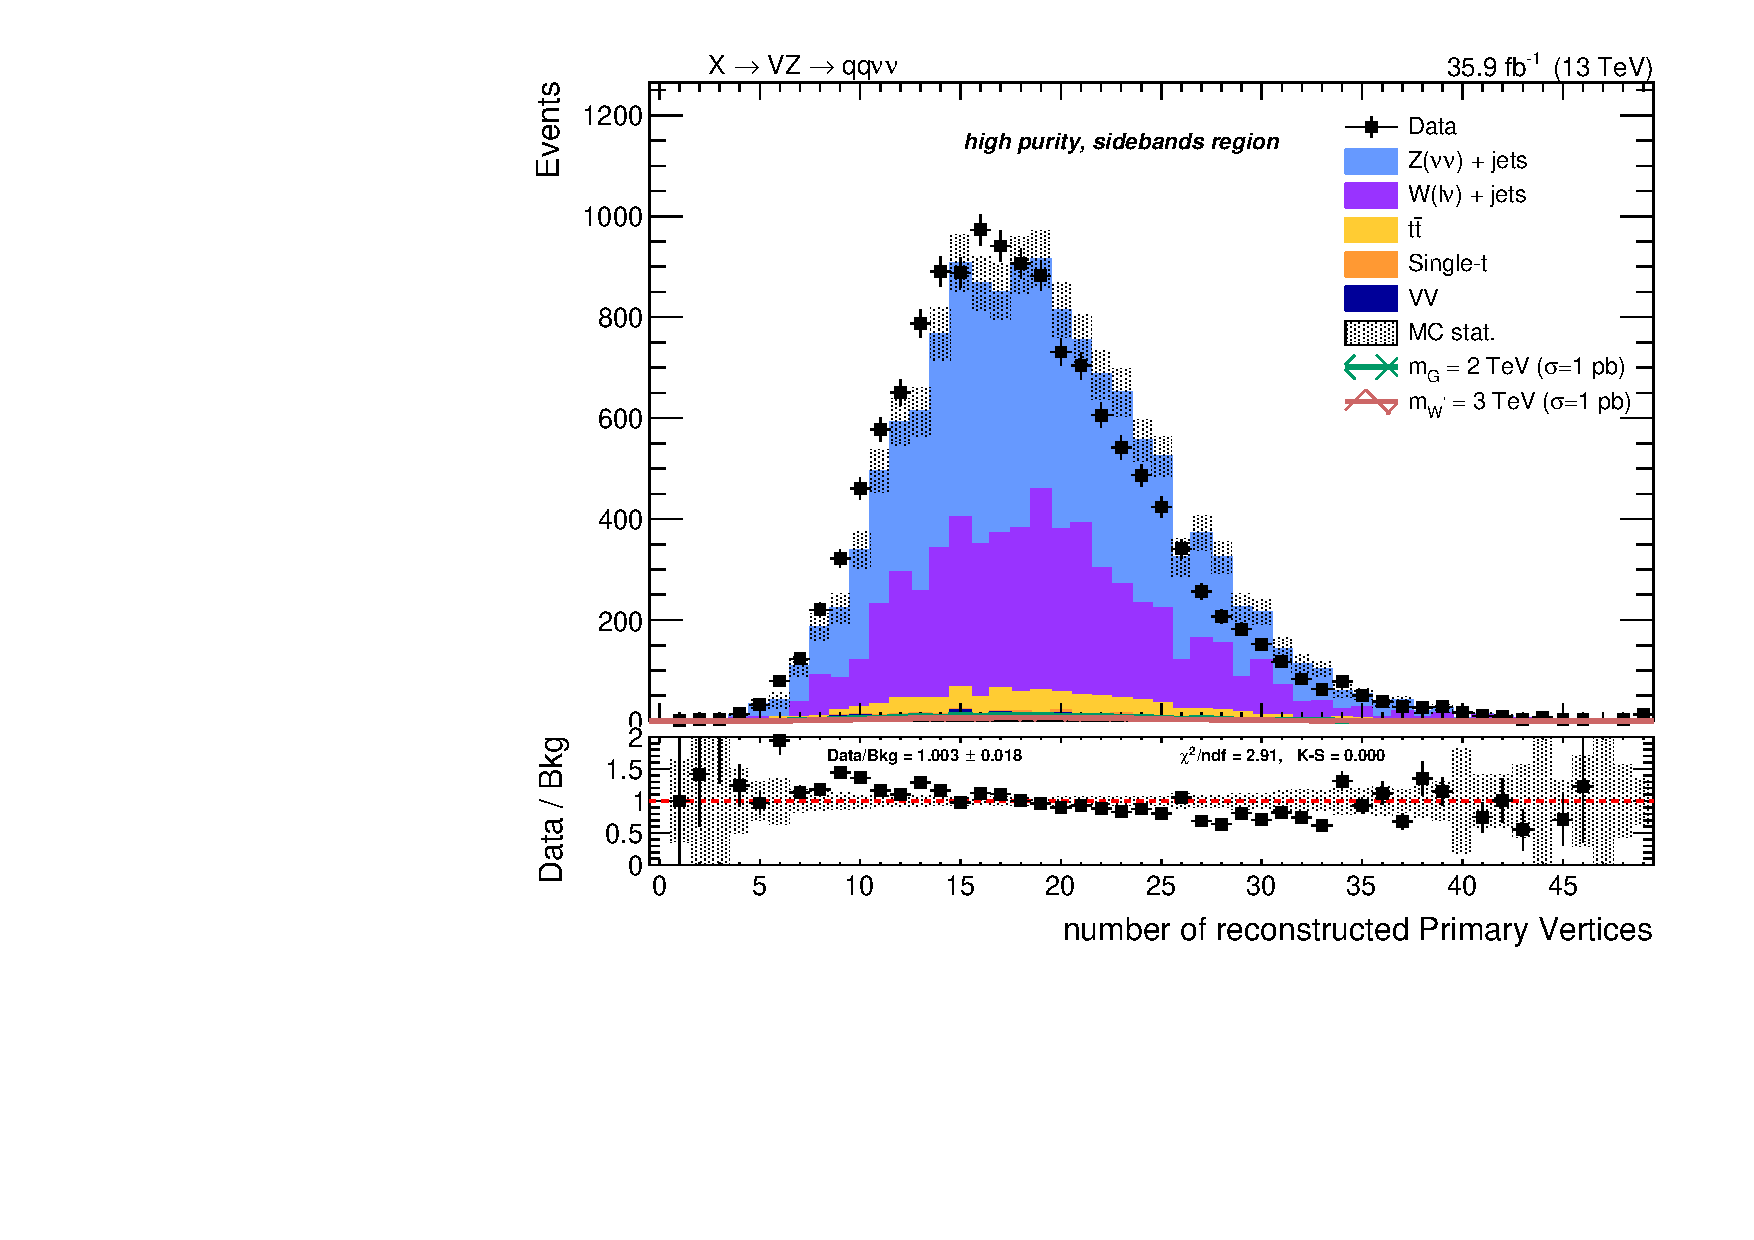
\includegraphics[width=0.495\textwidth]{plots/v9_thesis/XVZnnhpSB/nPV.pdf}
    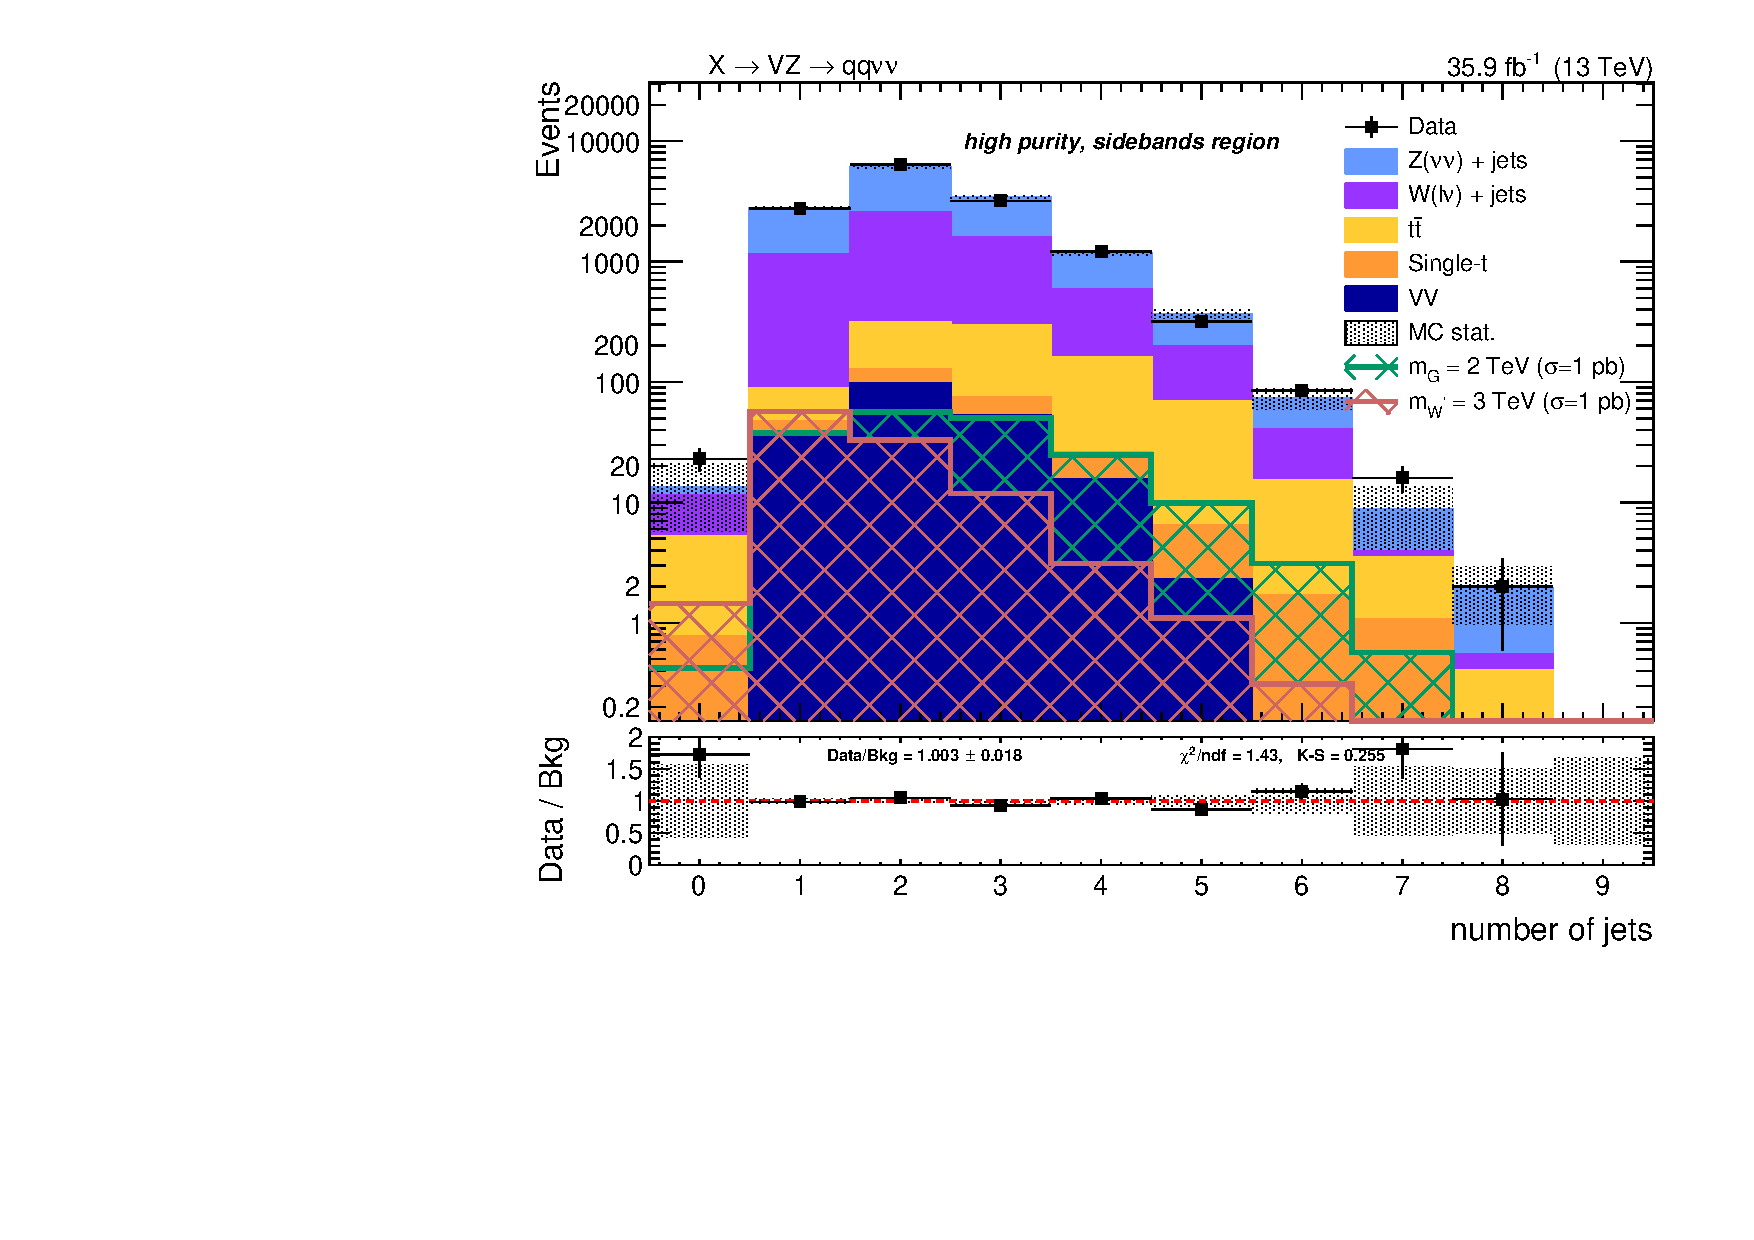
\includegraphics[width=0.495\textwidth]{plots/v9_thesis/XVZnnhpSB/nJets.pdf}

    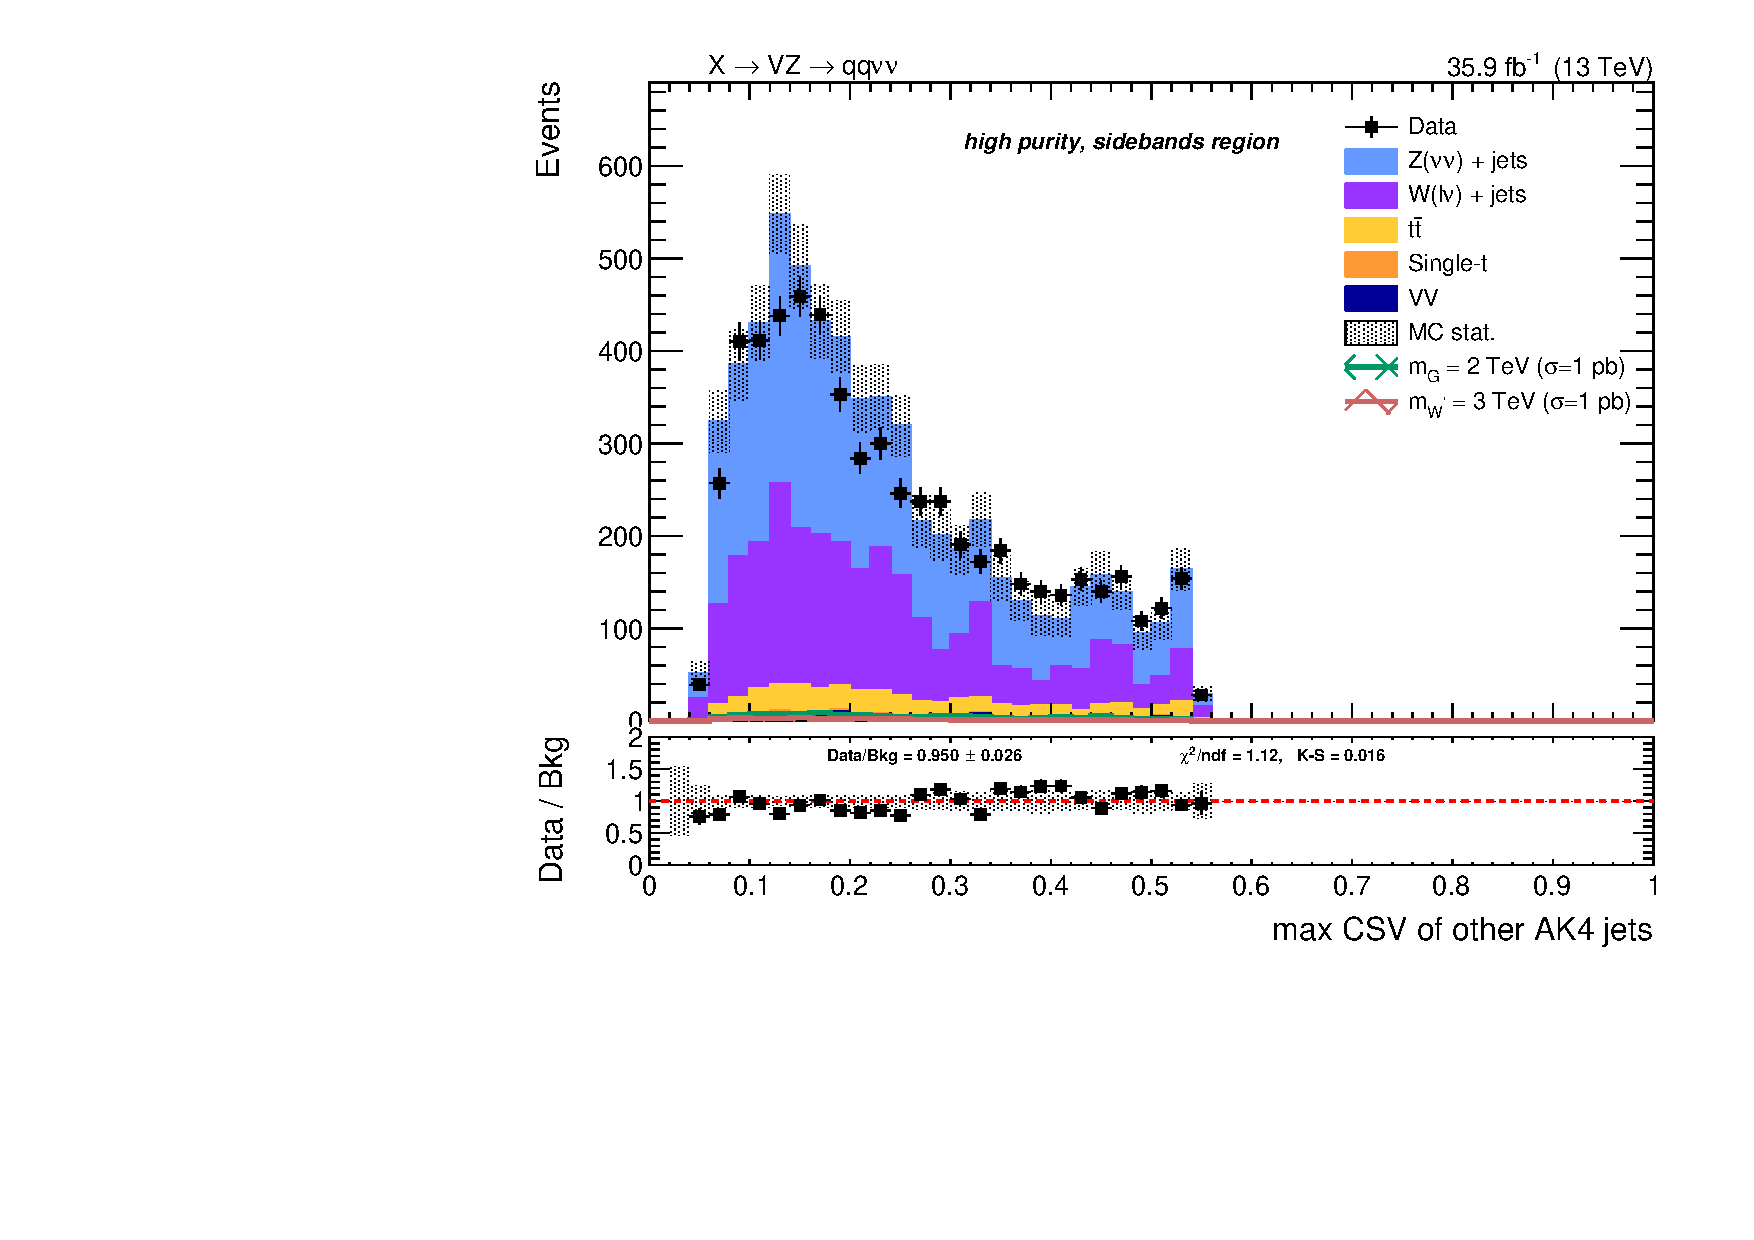
\includegraphics[width=0.495\textwidth]{plots/v9_thesis/XVZnnhpSB/MaxJetBTag.pdf}
    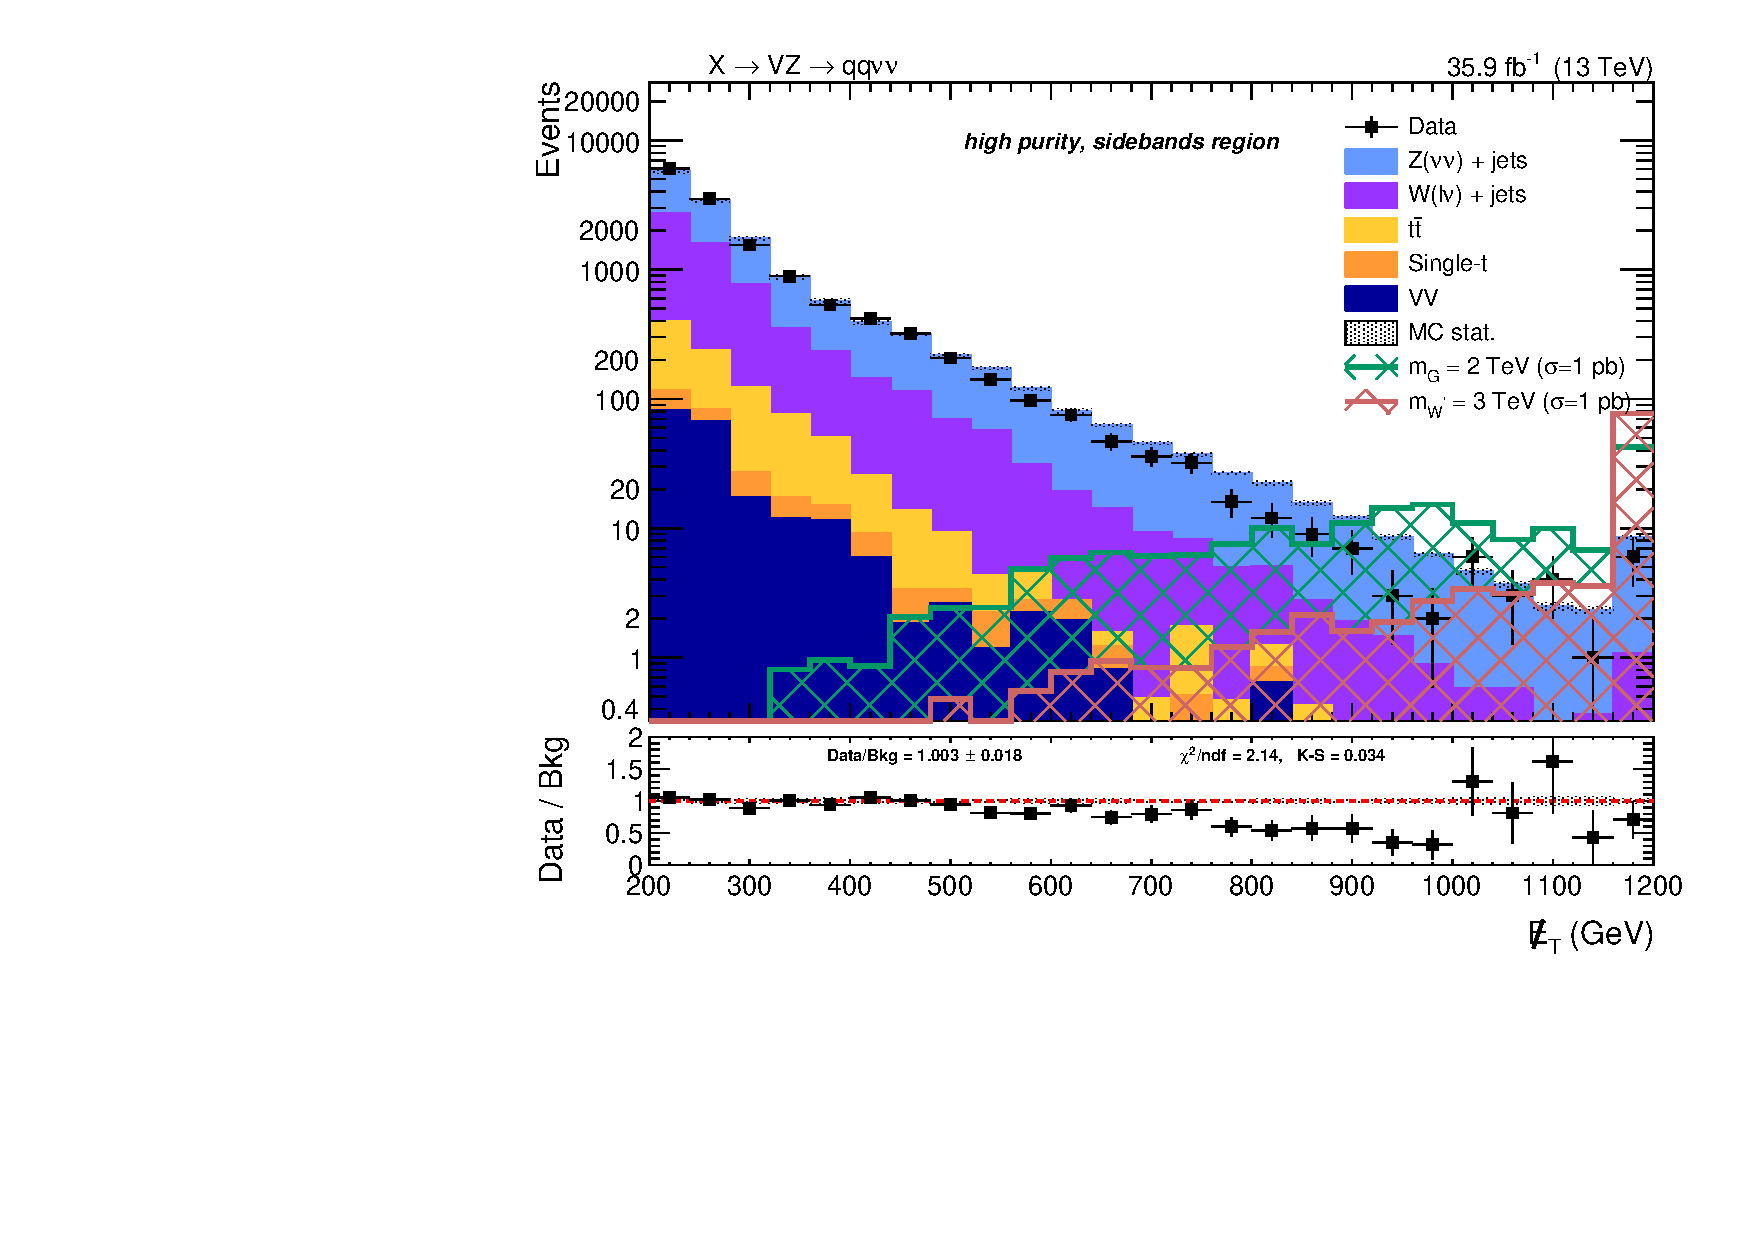
\includegraphics[width=0.495\textwidth]{plots/v9_thesis/XVZnnhpSB/MEt_pt.pdf}

    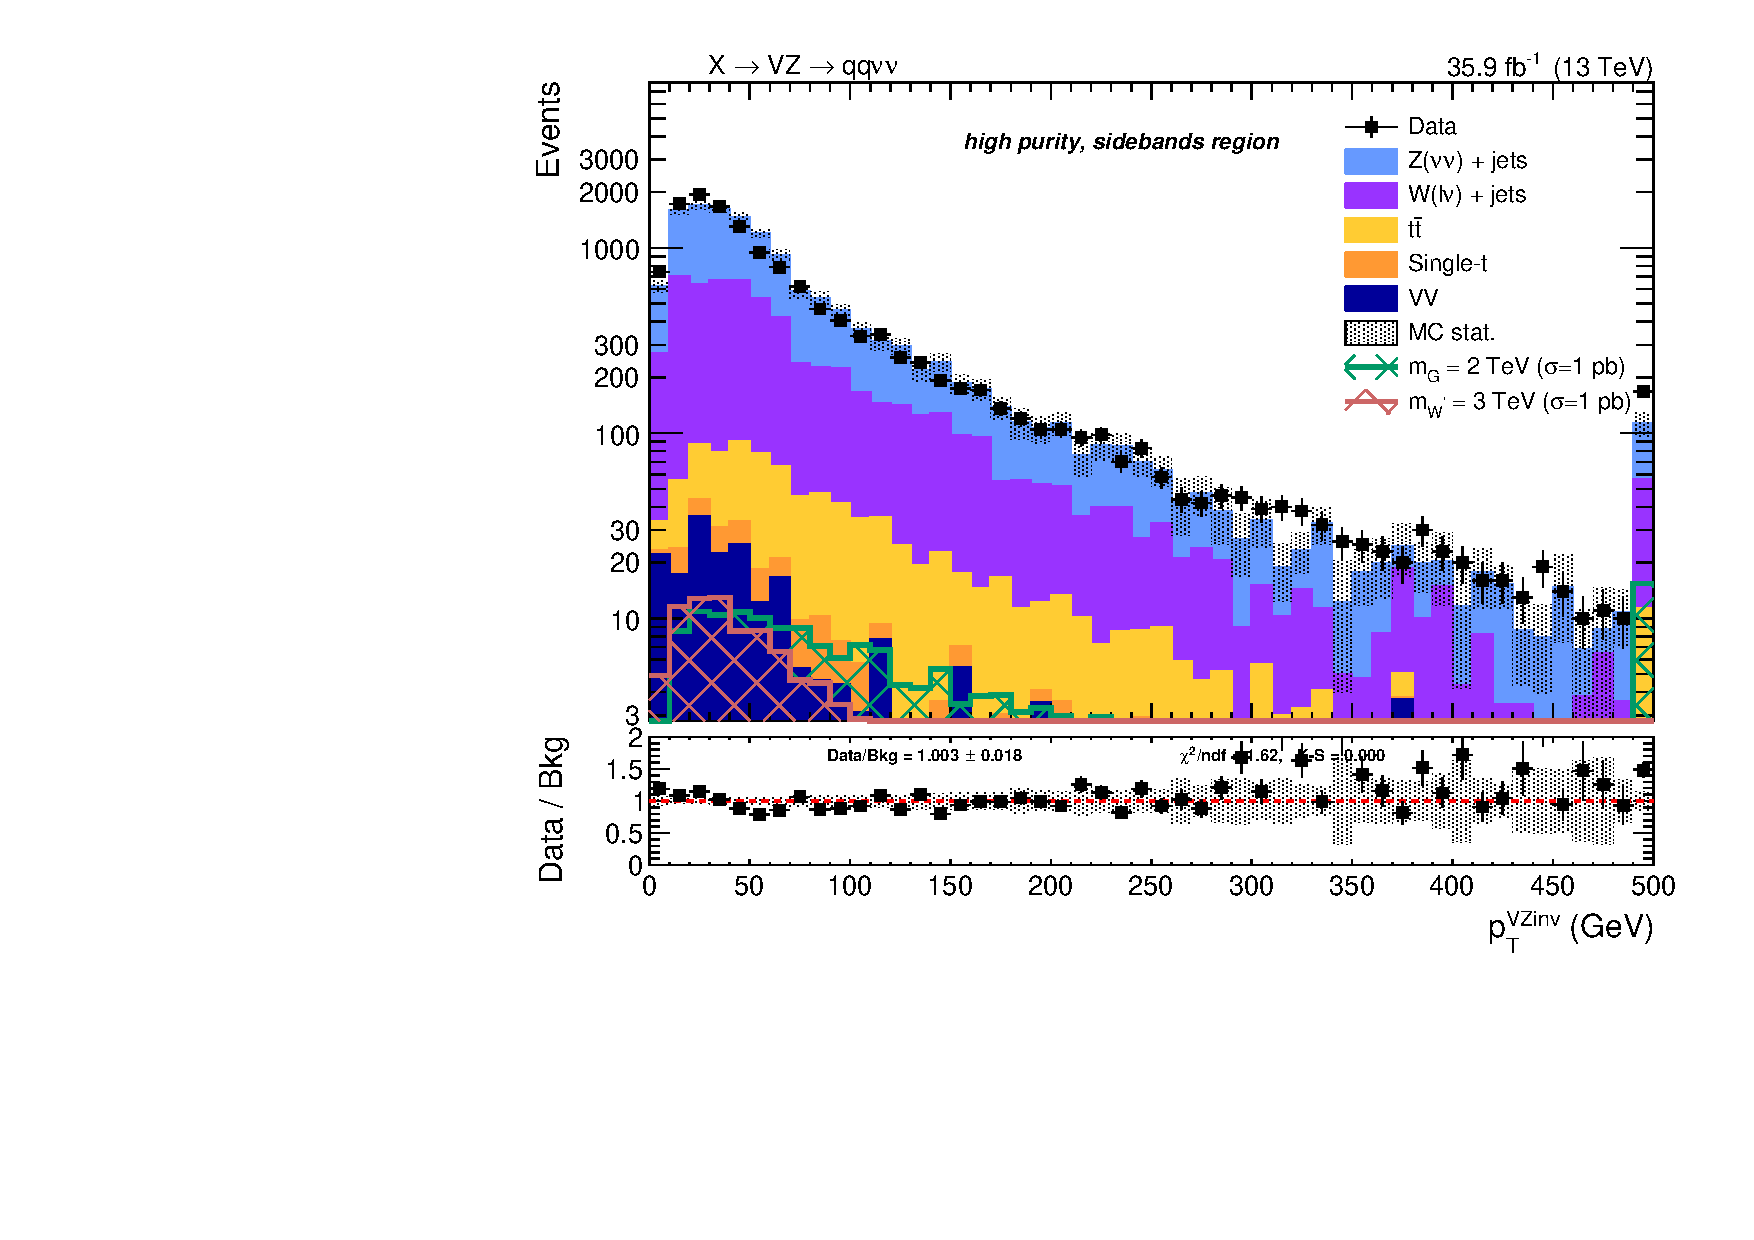
\includegraphics[width=0.495\textwidth]{plots/v9_thesis/XVZnnhpSB/X_pt.pdf}
    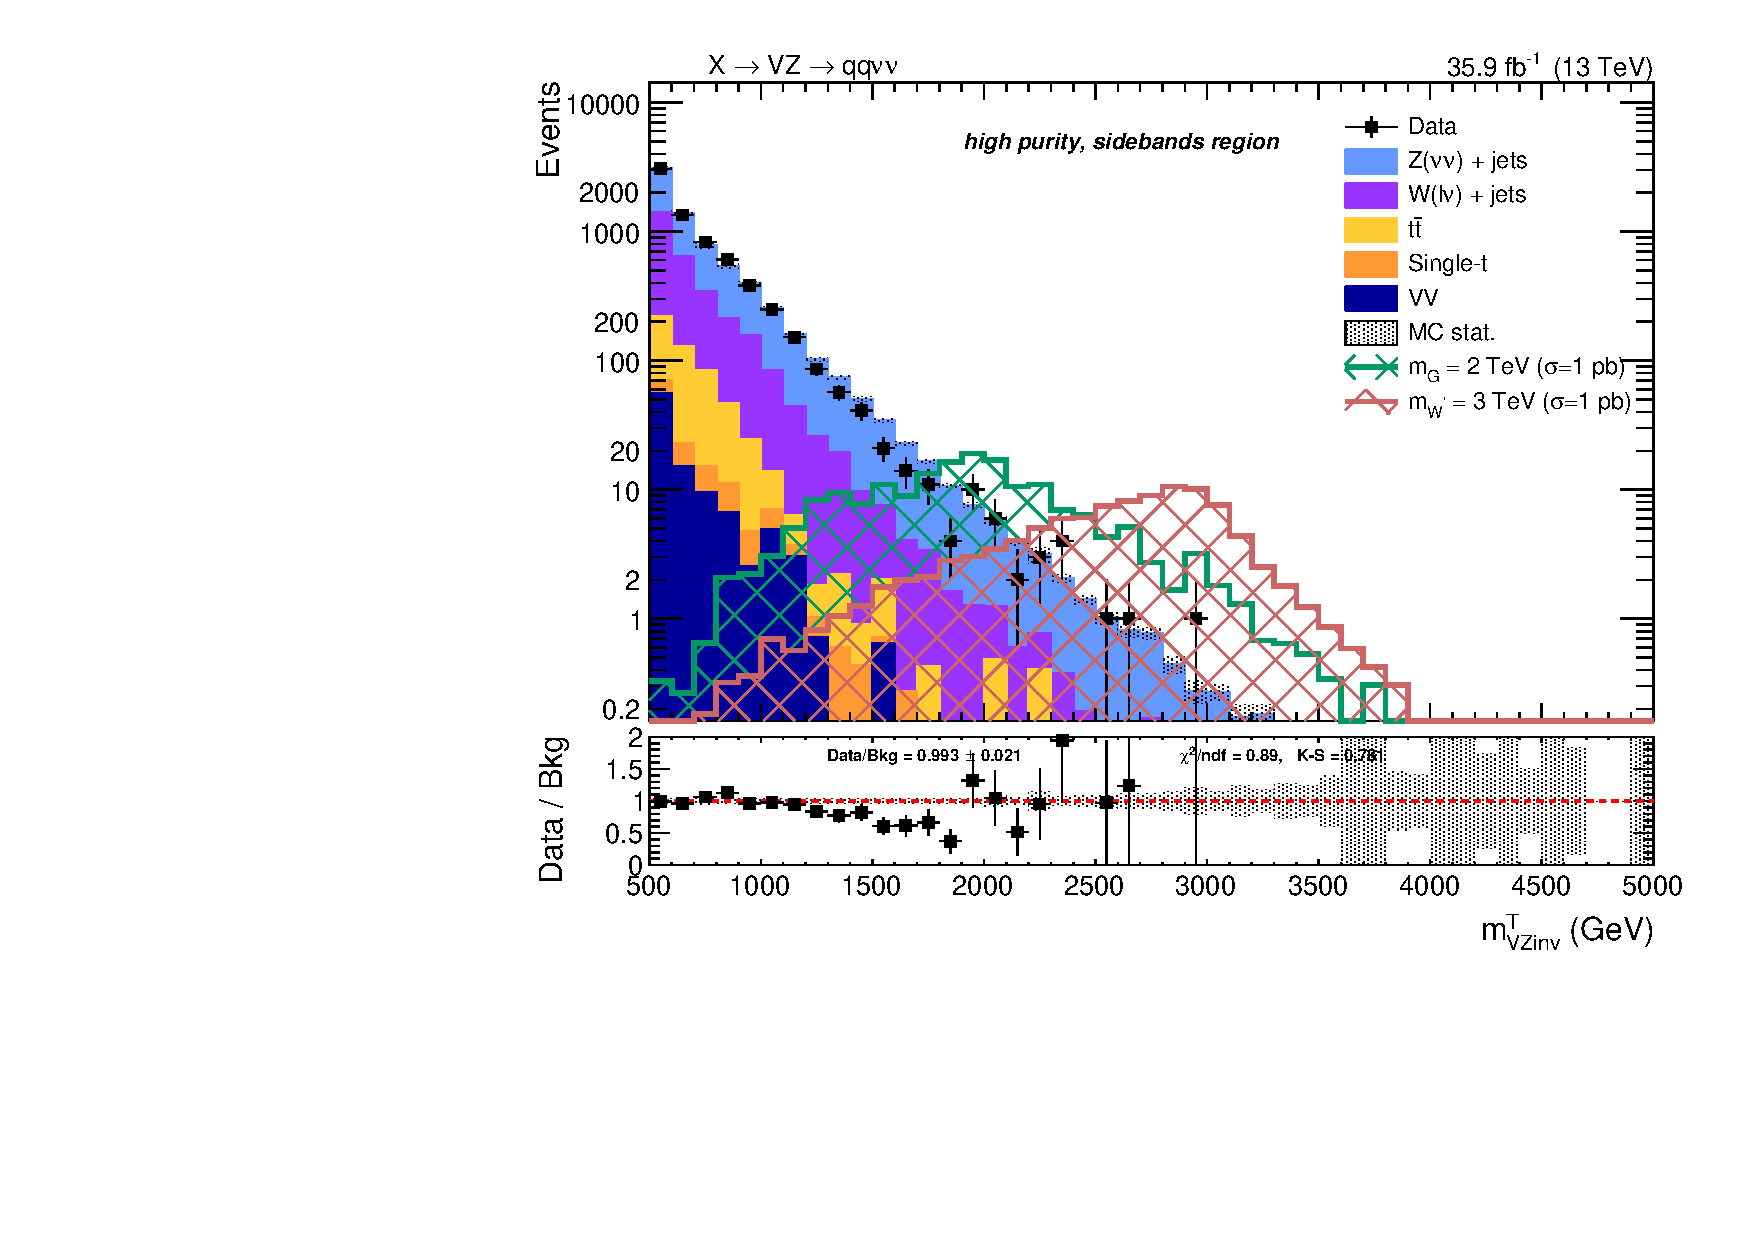
\includegraphics[width=0.495\textwidth]{plots/v9_thesis/XVZnnhpSB/X_tmass.pdf}

    \caption{Top: number of reconstructed primary vertices (left) and number of AK4 jets in the event (right). Center: distribution of the b-tagging multivariate discriminant for the AK4 jets not included in the \V jet cone (left) and \MET distribution (right). Bottom: \pt of the \VZ candidate (left) and transverse mass of the \VZ candidate (right). Events are selected with the \emph{high-purity sidebands} selection, and simulated backgrounds are normalized to luminosity.}
%\label{fig:XZhll_N}
  \end{center}
\end{figure}

\clearpage

%plot scelti
%lpSR

\begin{figure}[!htb]
  \begin{center}
    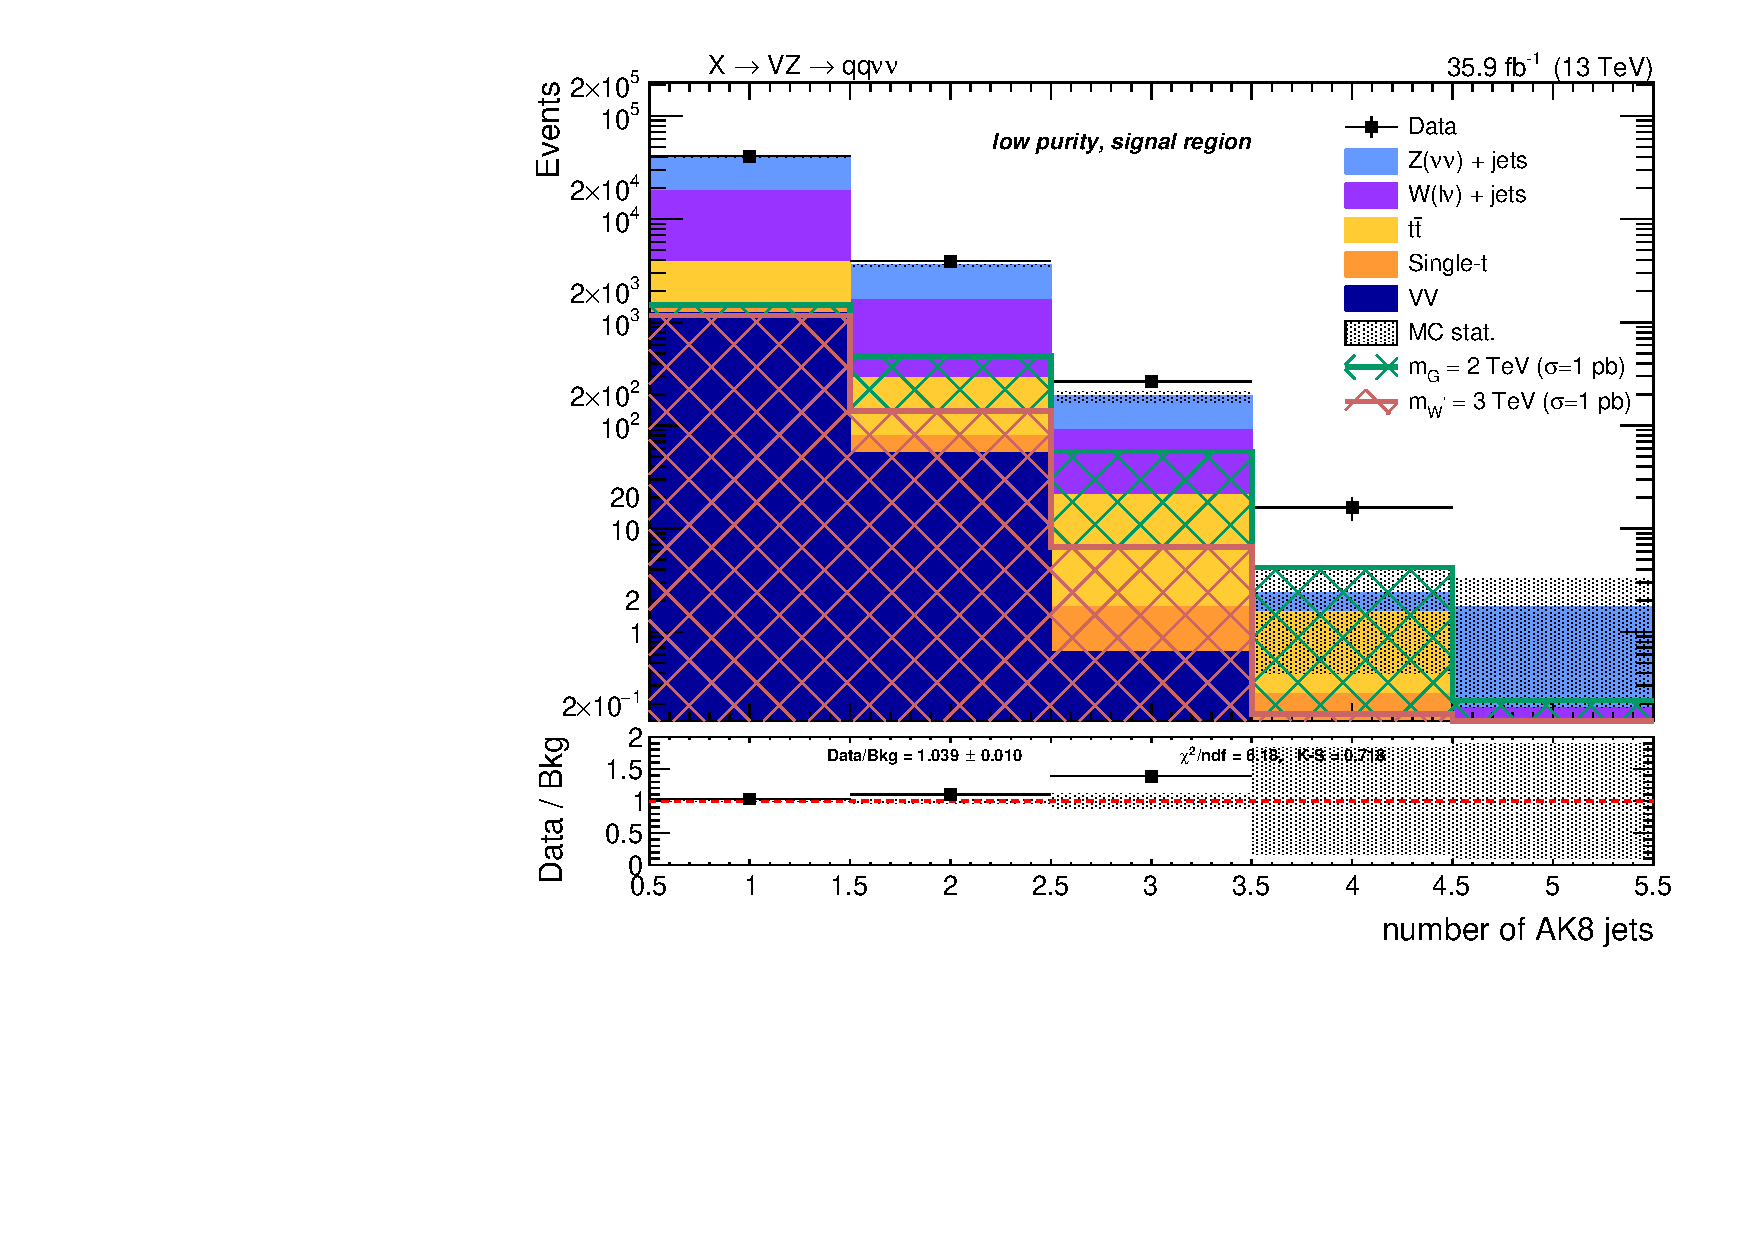
\includegraphics[width=0.495\textwidth]{plots/v9_thesis/XVZnnlpSR/nFatJets.pdf}  
    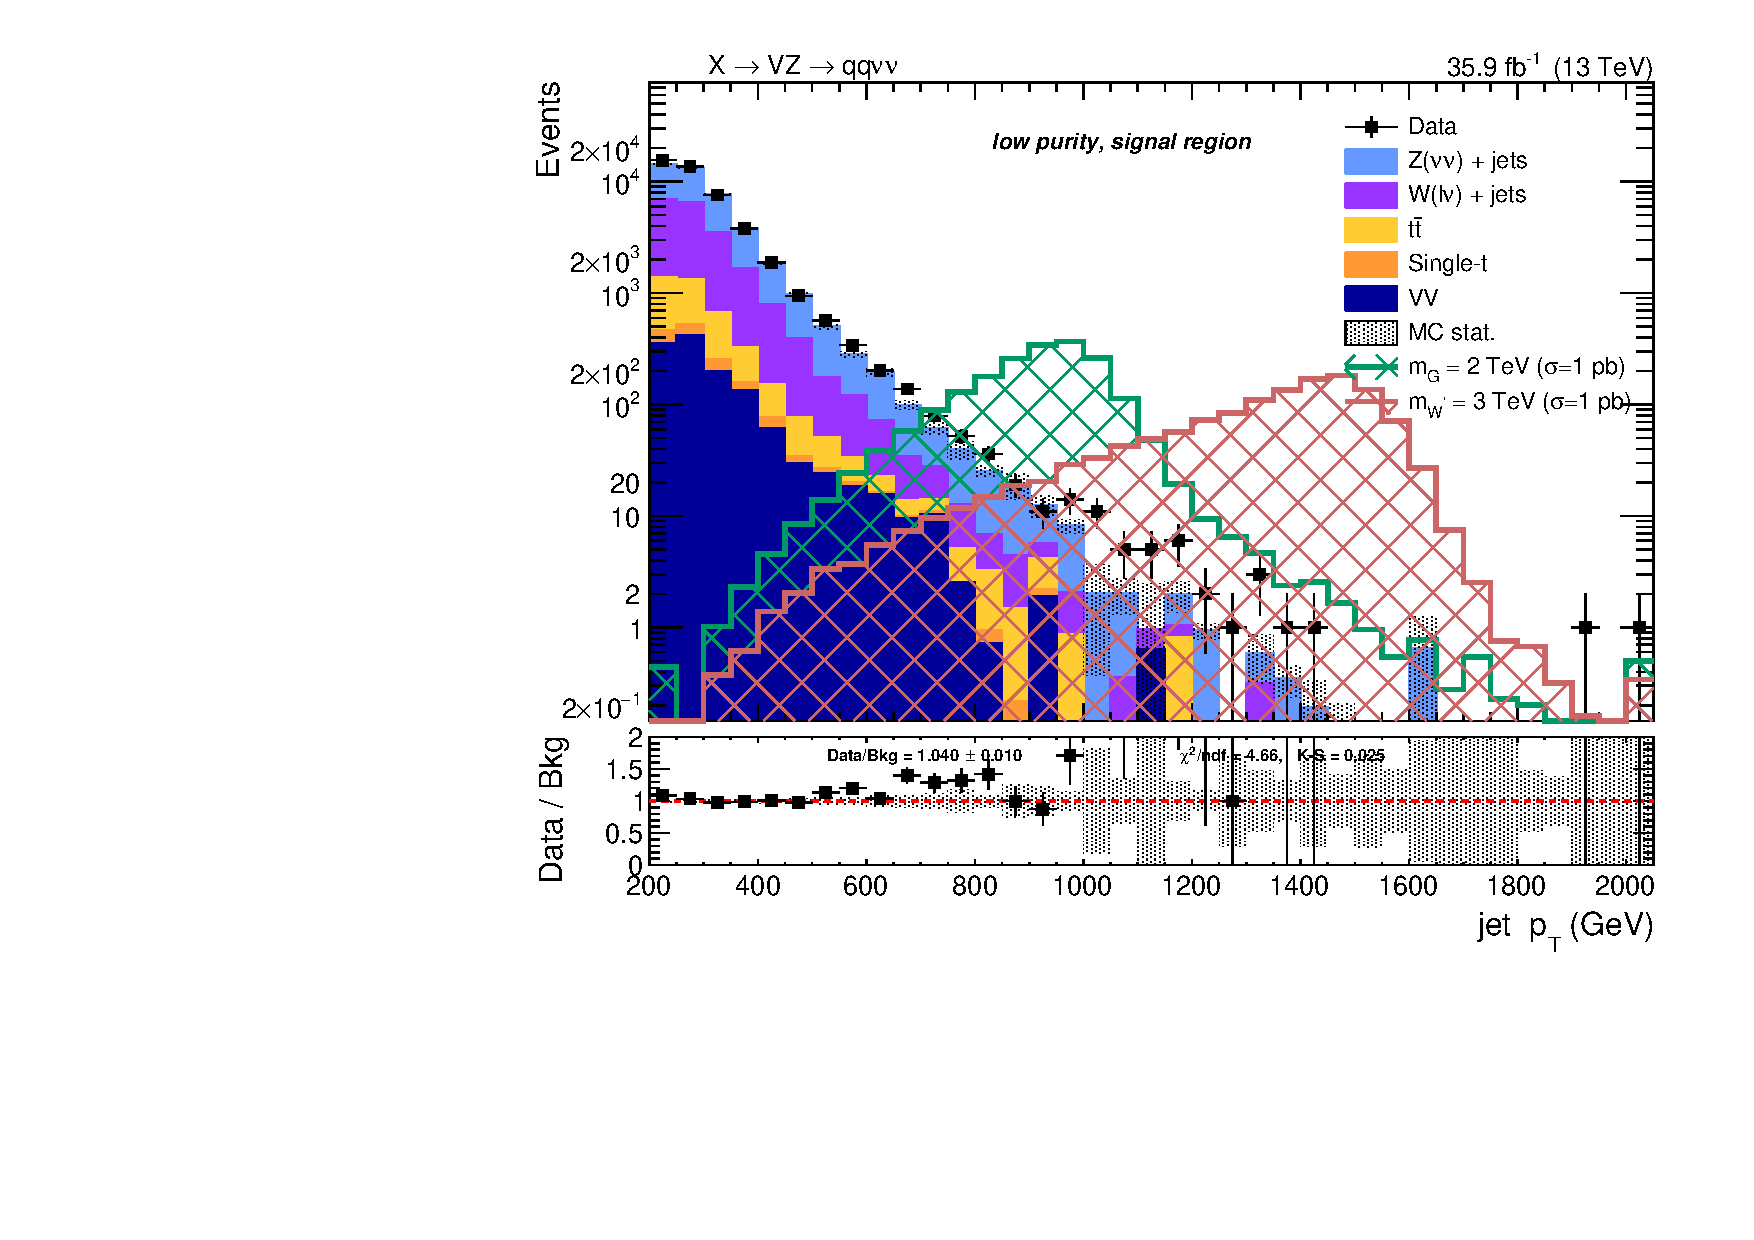
\includegraphics[width=0.495\textwidth]{plots/v9_thesis/XVZnnlpSR/FatJet1_pt.pdf}
    
    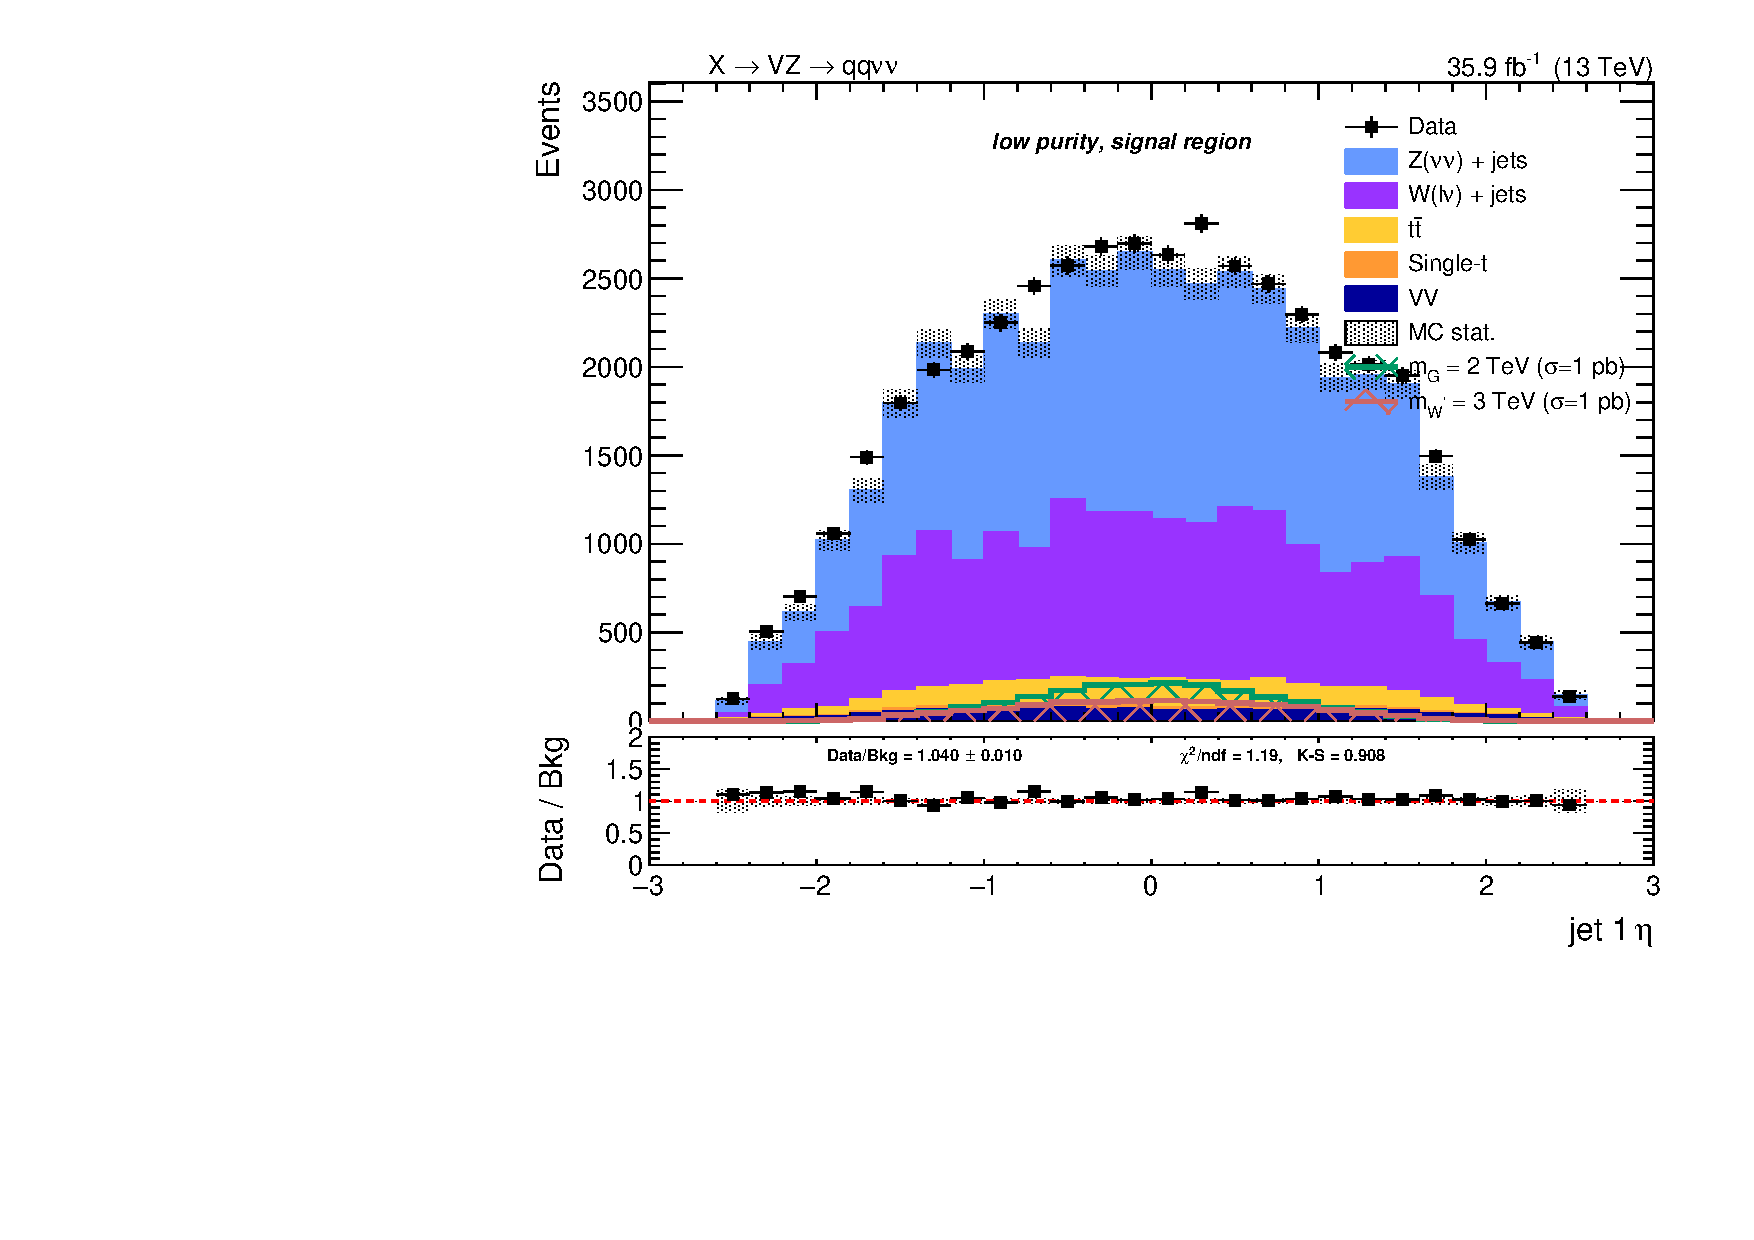
\includegraphics[width=0.495\textwidth]{plots/v9_thesis/XVZnnlpSR/FatJet1_eta.pdf}
    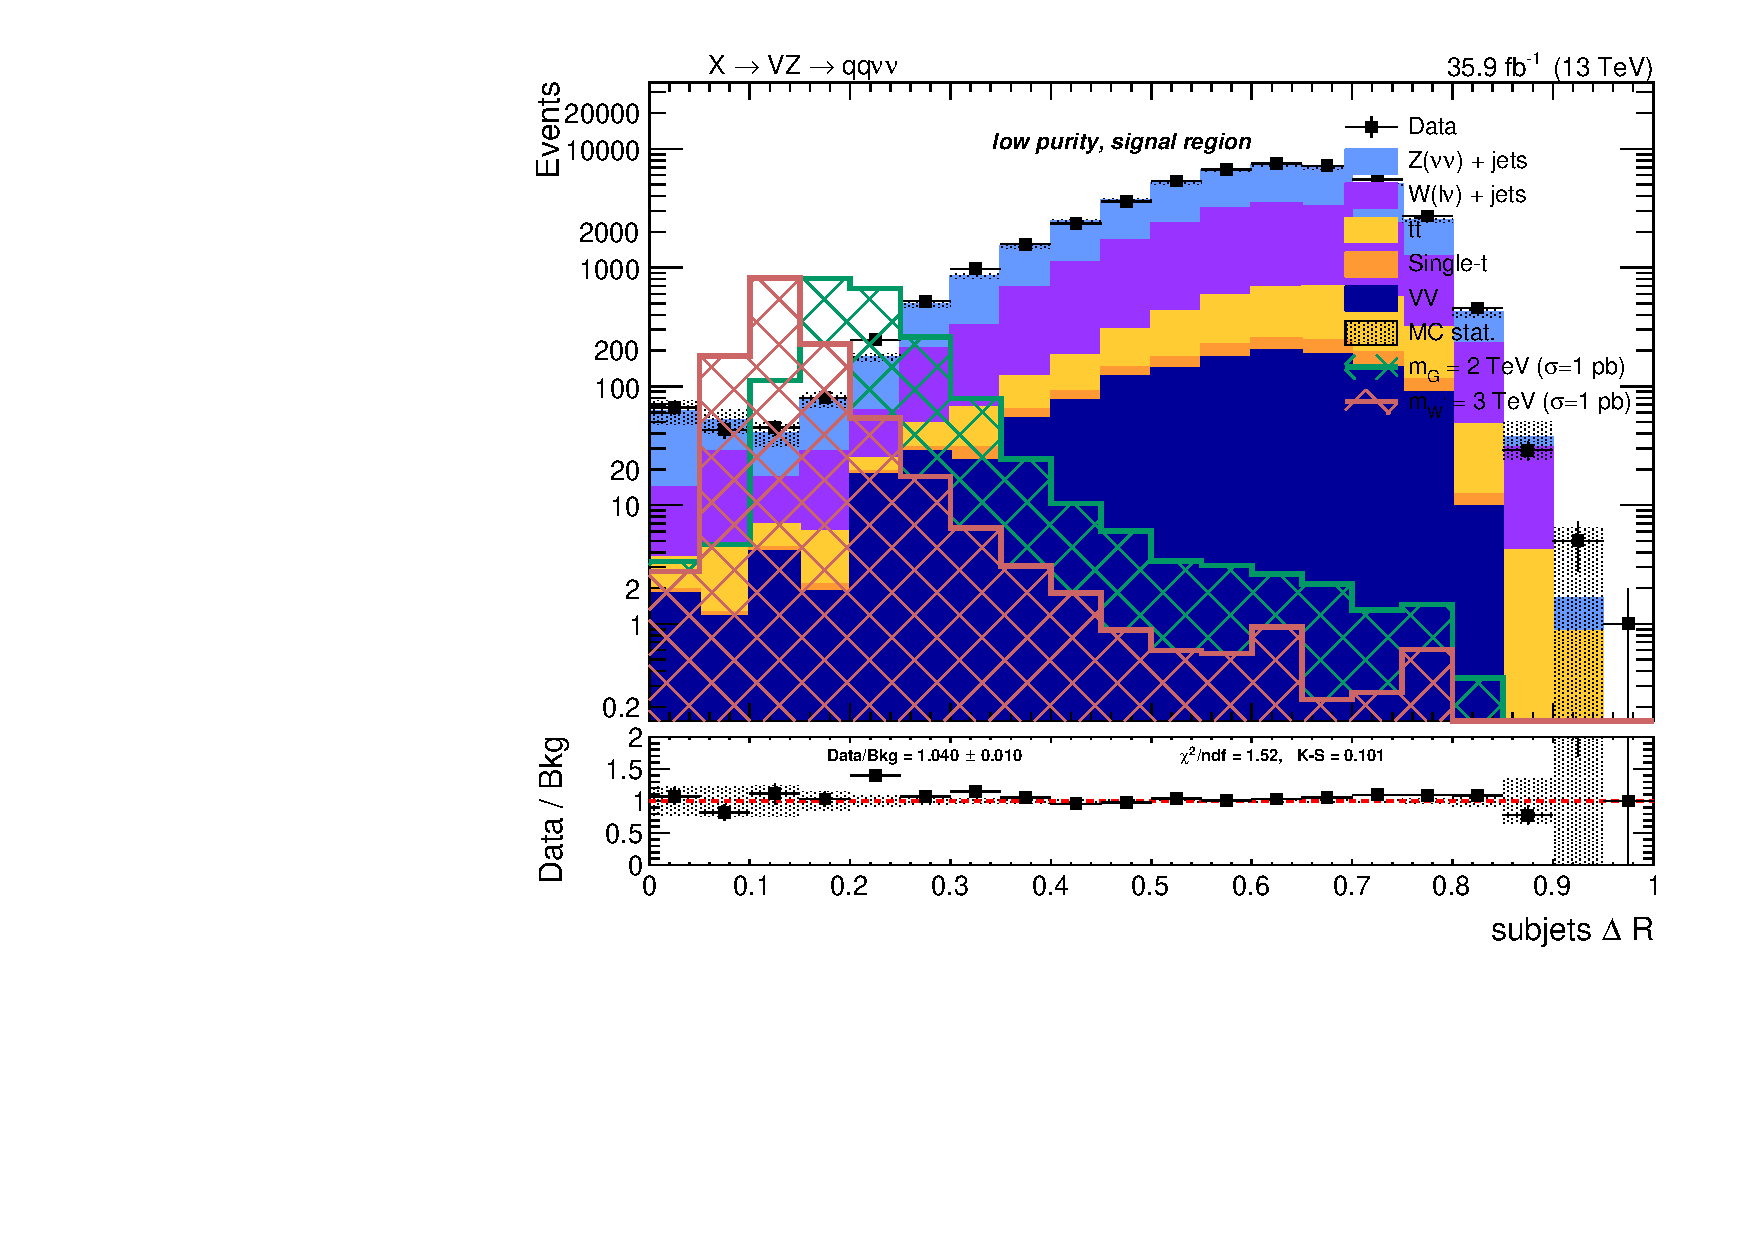
\includegraphics[width=0.495\textwidth]{plots/v9_thesis/XVZnnlpSR/FatJet1_dR.pdf}

    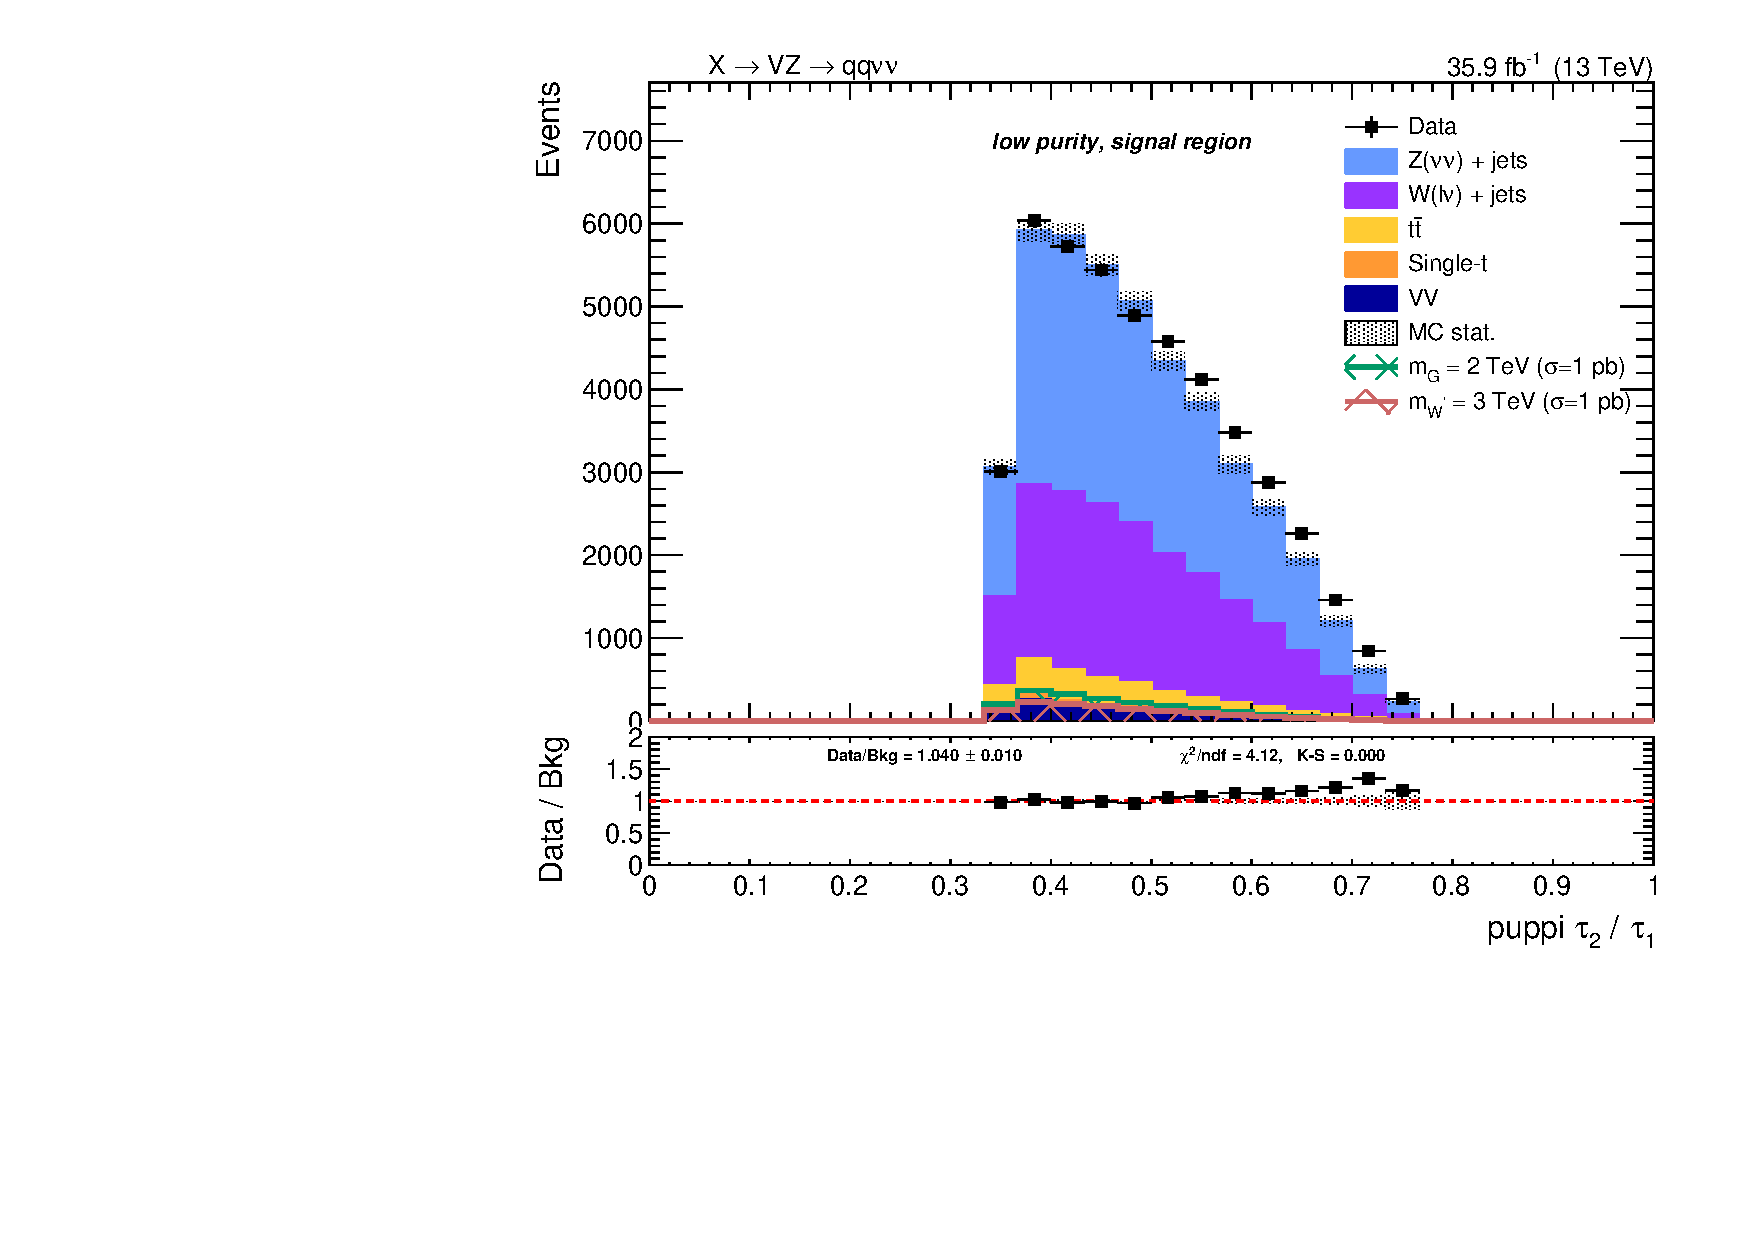
\includegraphics[width=0.495\textwidth]{plots/v9_thesis/XVZnnlpSR/FatJet1_puppiTau21.pdf}
    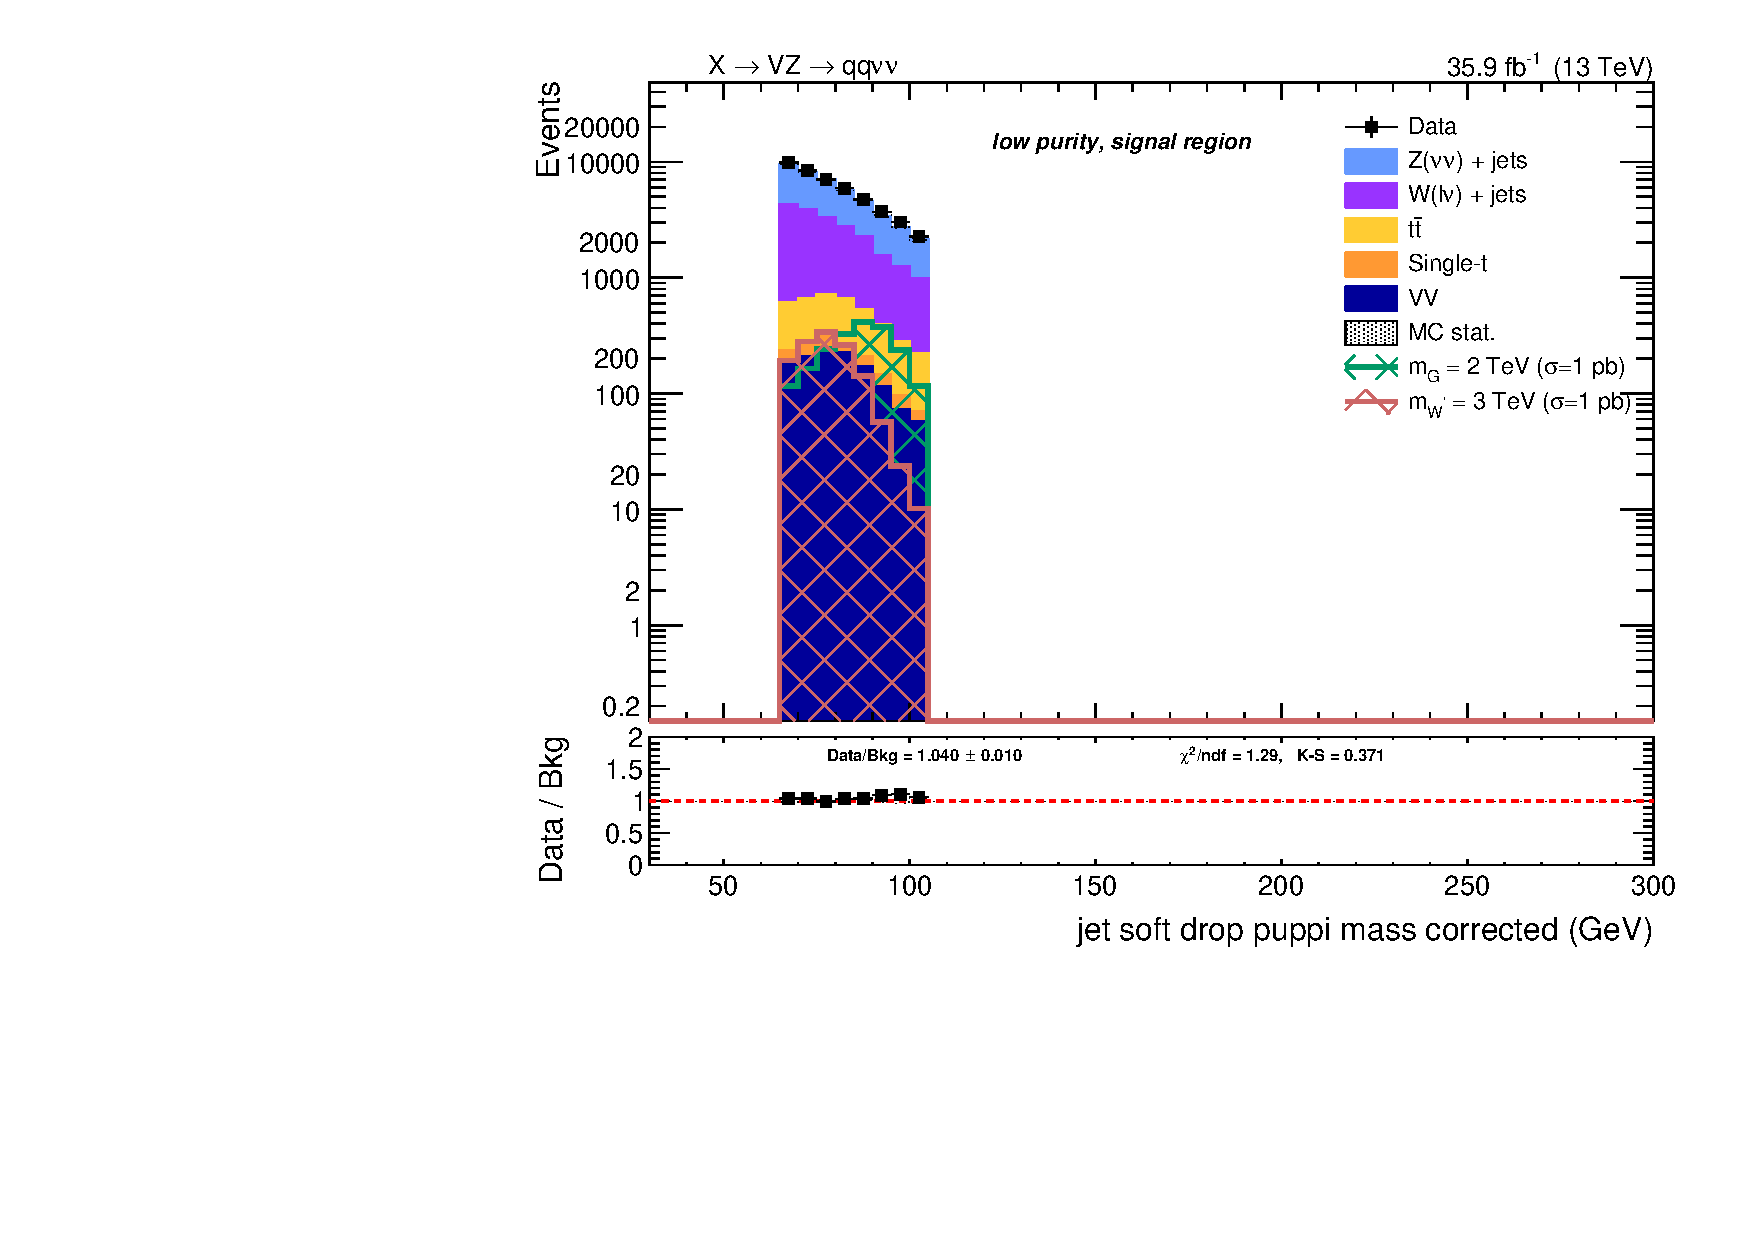
\includegraphics[width=0.495\textwidth]{plots/v9_thesis/XVZnnlpSR/FatJet1_softdropPuppiMassCorr.pdf}

    \caption{Top: number of AK8 jets in the event (left) and \V jet candidate \pt (right). Center: \V jet candidate $\eta$ (left) and angular separation $\Delta R$ between the constituents leading subjets (right). Bottom: \V jet candidate $\tau_{21}$ subjettiness after PUPPI correction (left) and \V jet candidate soft drop PUPPI mass (right). Events are selected with the \emph{low-purity signal region} selection, and simulated backgrounds are normalized to luminosity.}
%\label{fig:XZhll_N}
  \end{center}
\end{figure}

\clearpage

\begin{figure}[!htb]
  \begin{center}  
    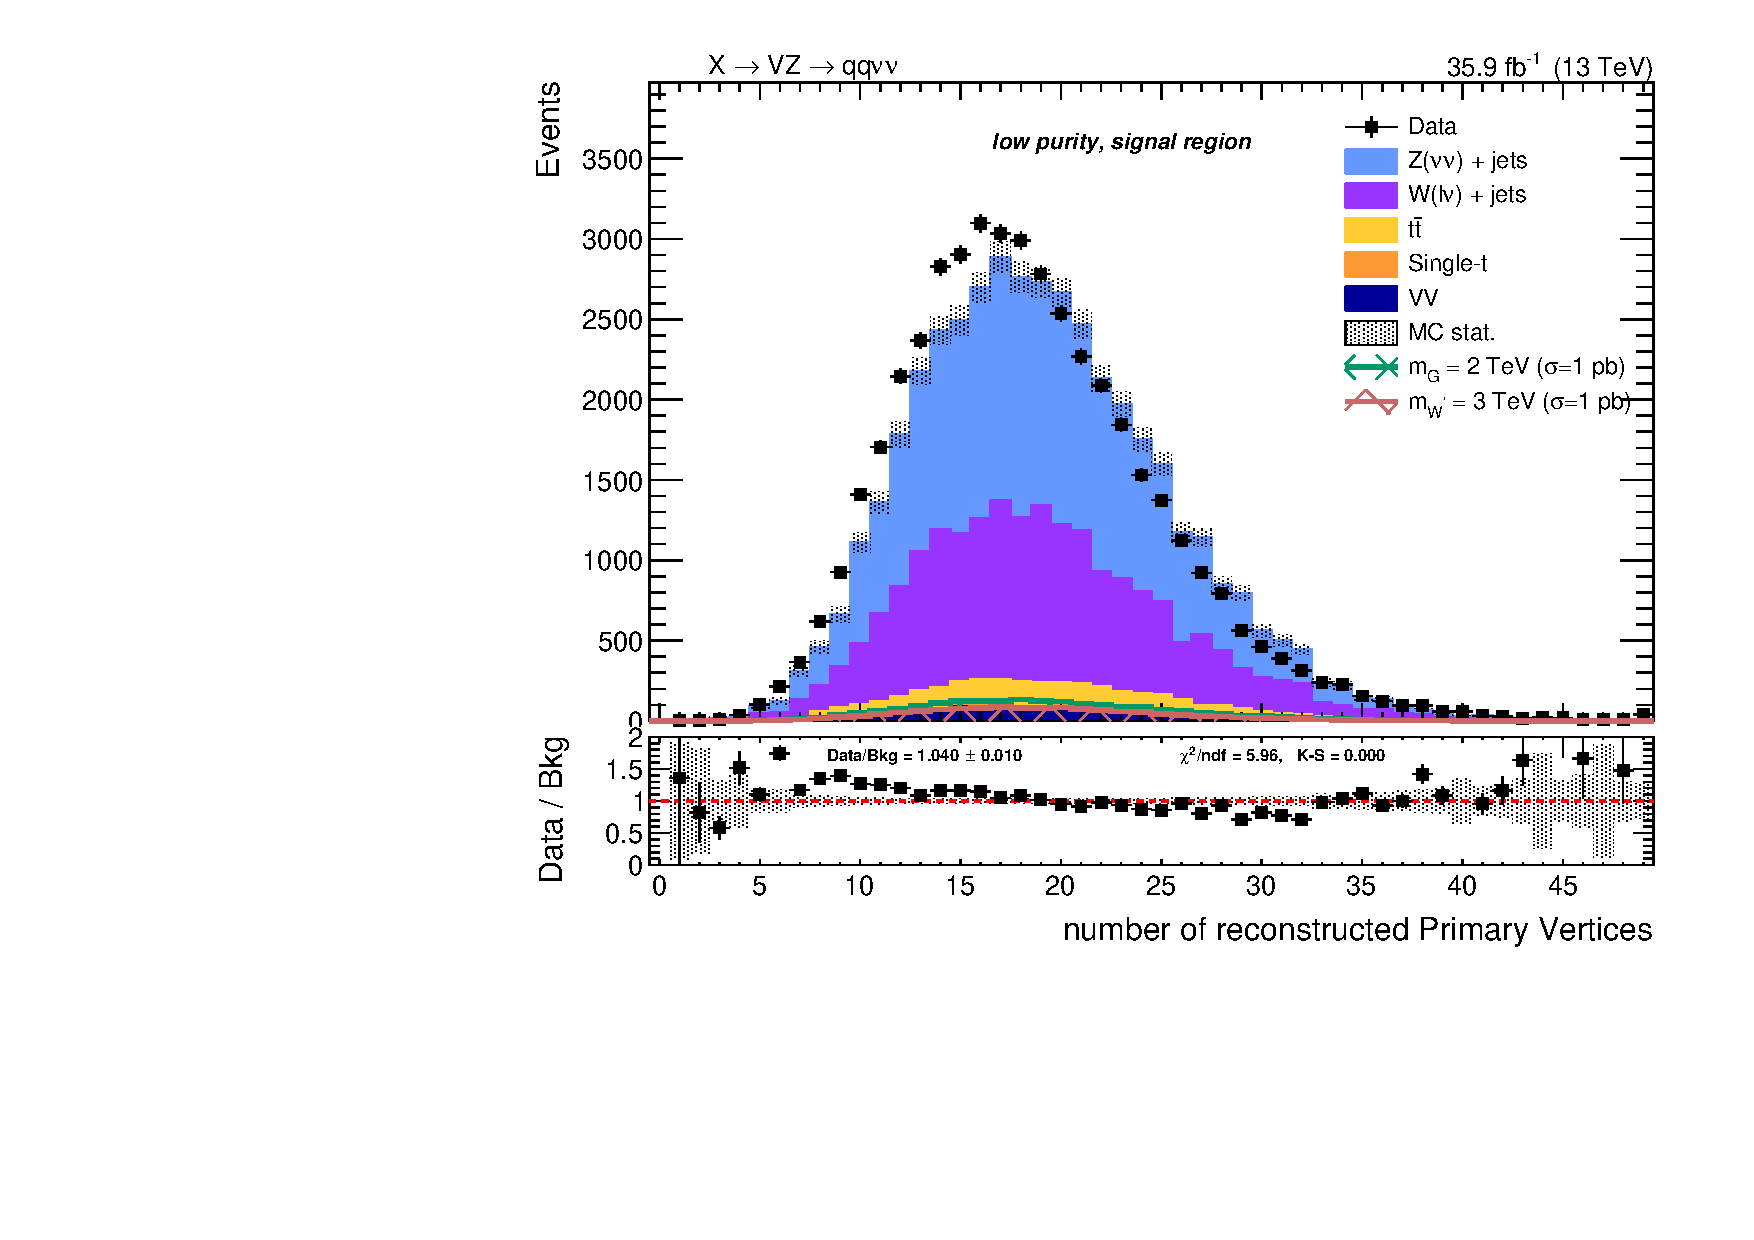
\includegraphics[width=0.495\textwidth]{plots/v9_thesis/XVZnnlpSR/nPV.pdf}
    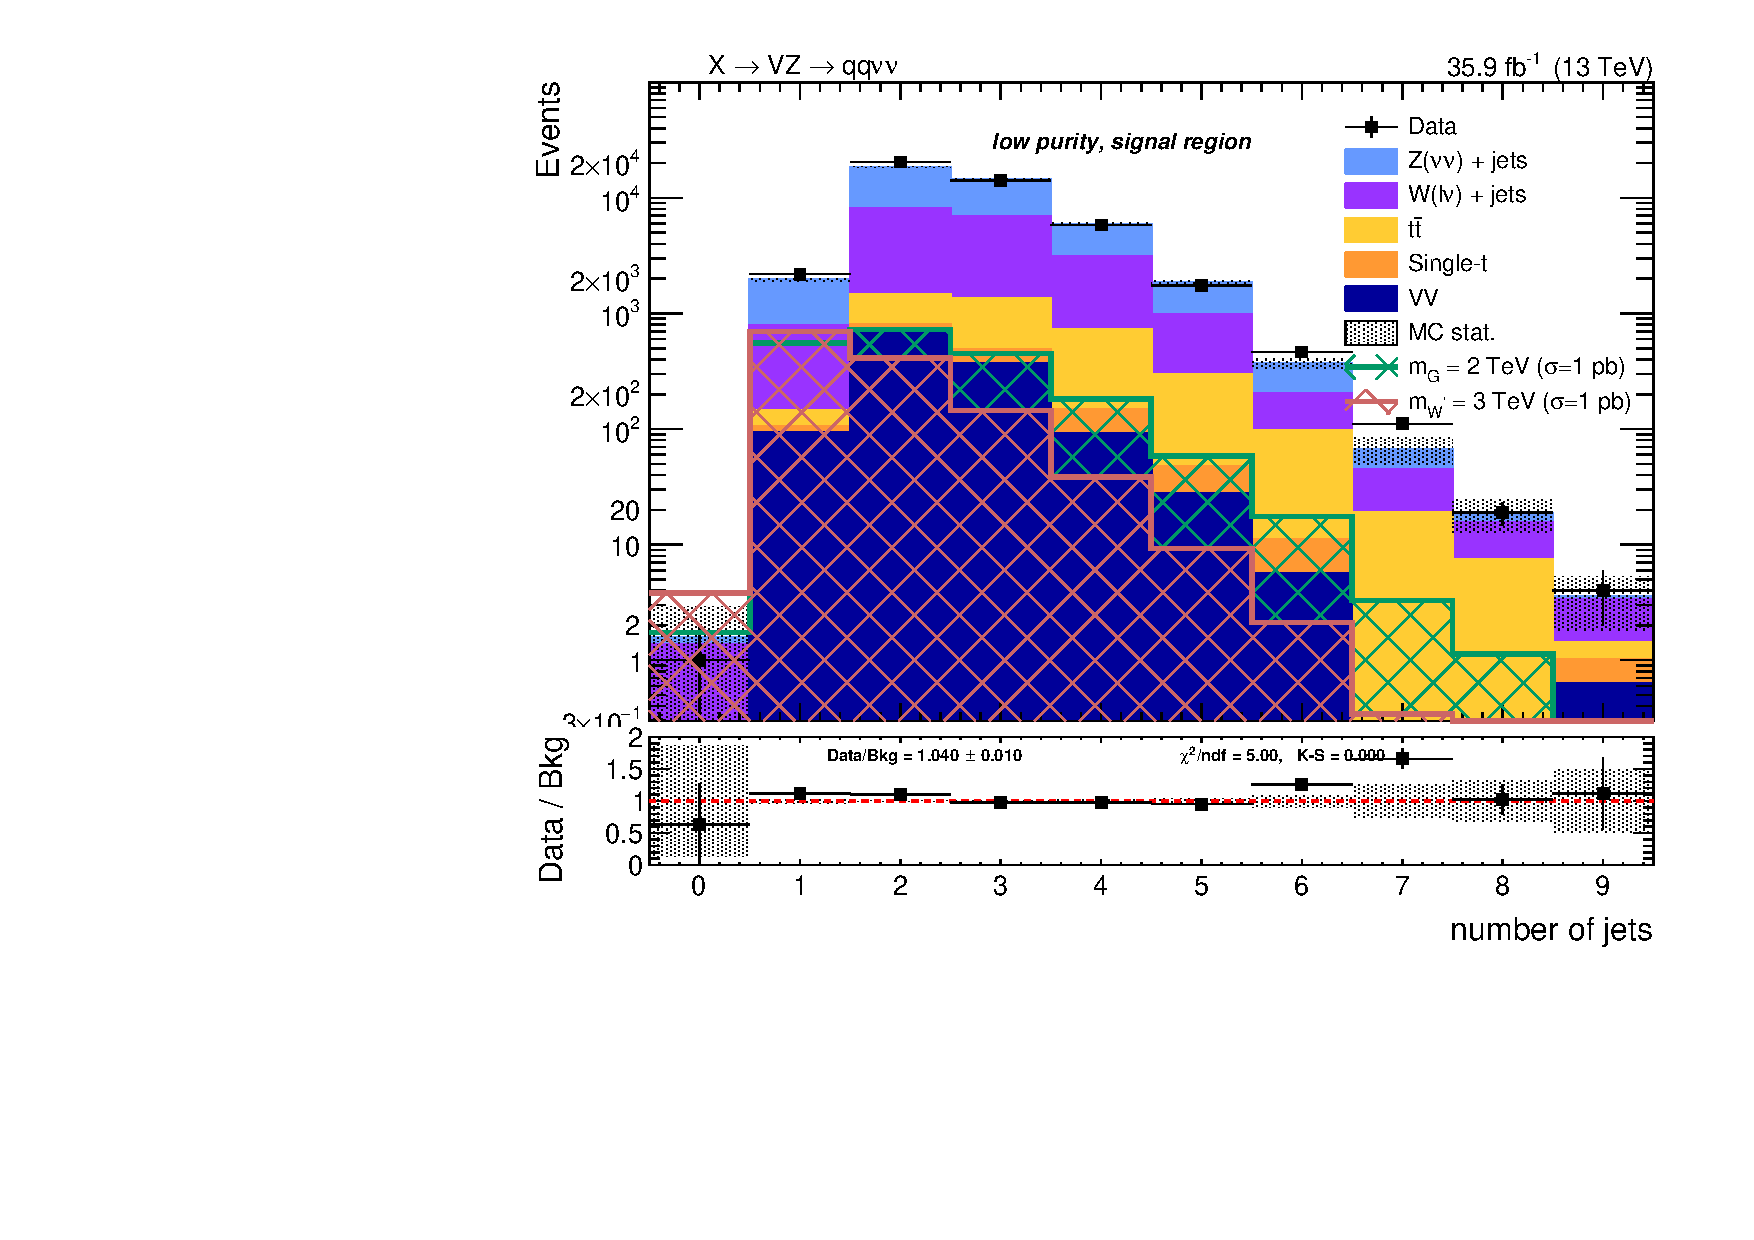
\includegraphics[width=0.495\textwidth]{plots/v9_thesis/XVZnnlpSR/nJets.pdf}

    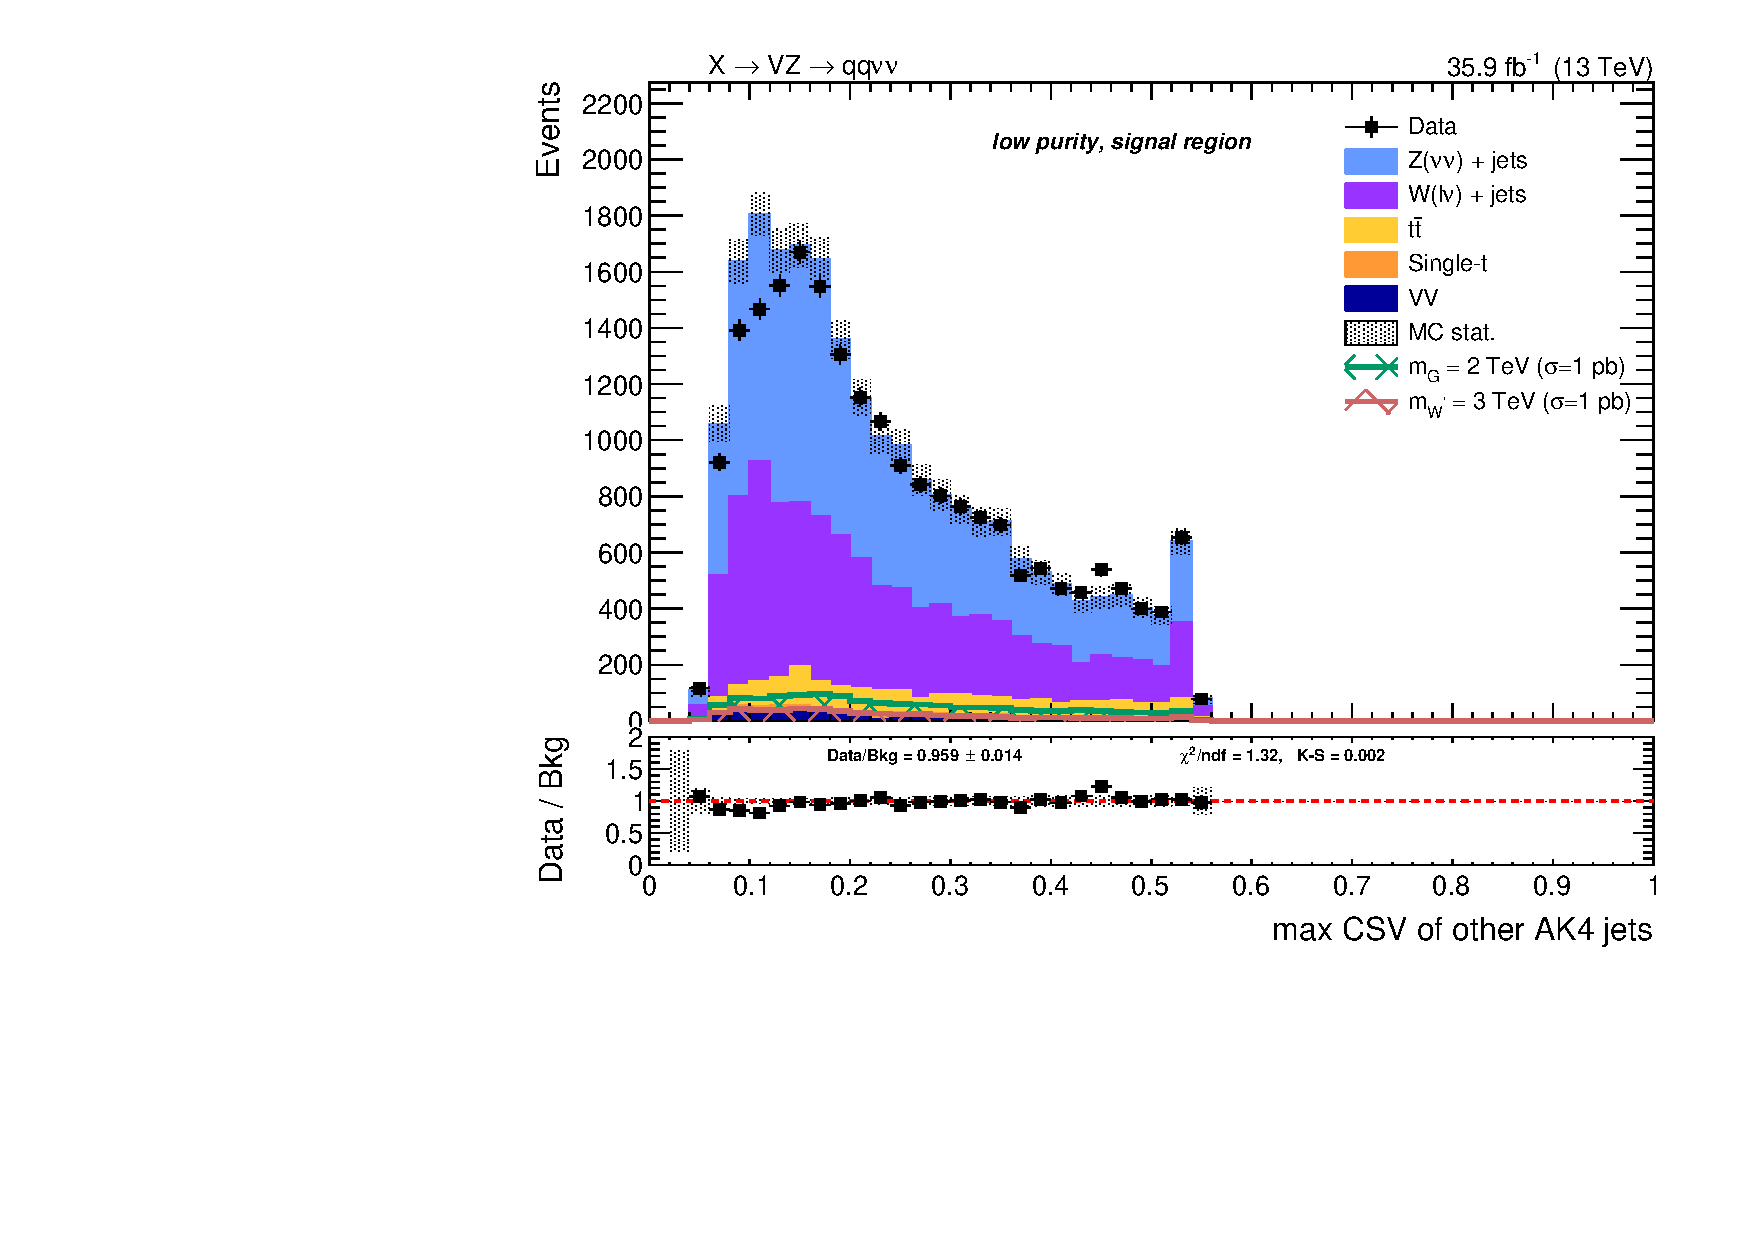
\includegraphics[width=0.495\textwidth]{plots/v9_thesis/XVZnnlpSR/MaxJetBTag.pdf}
    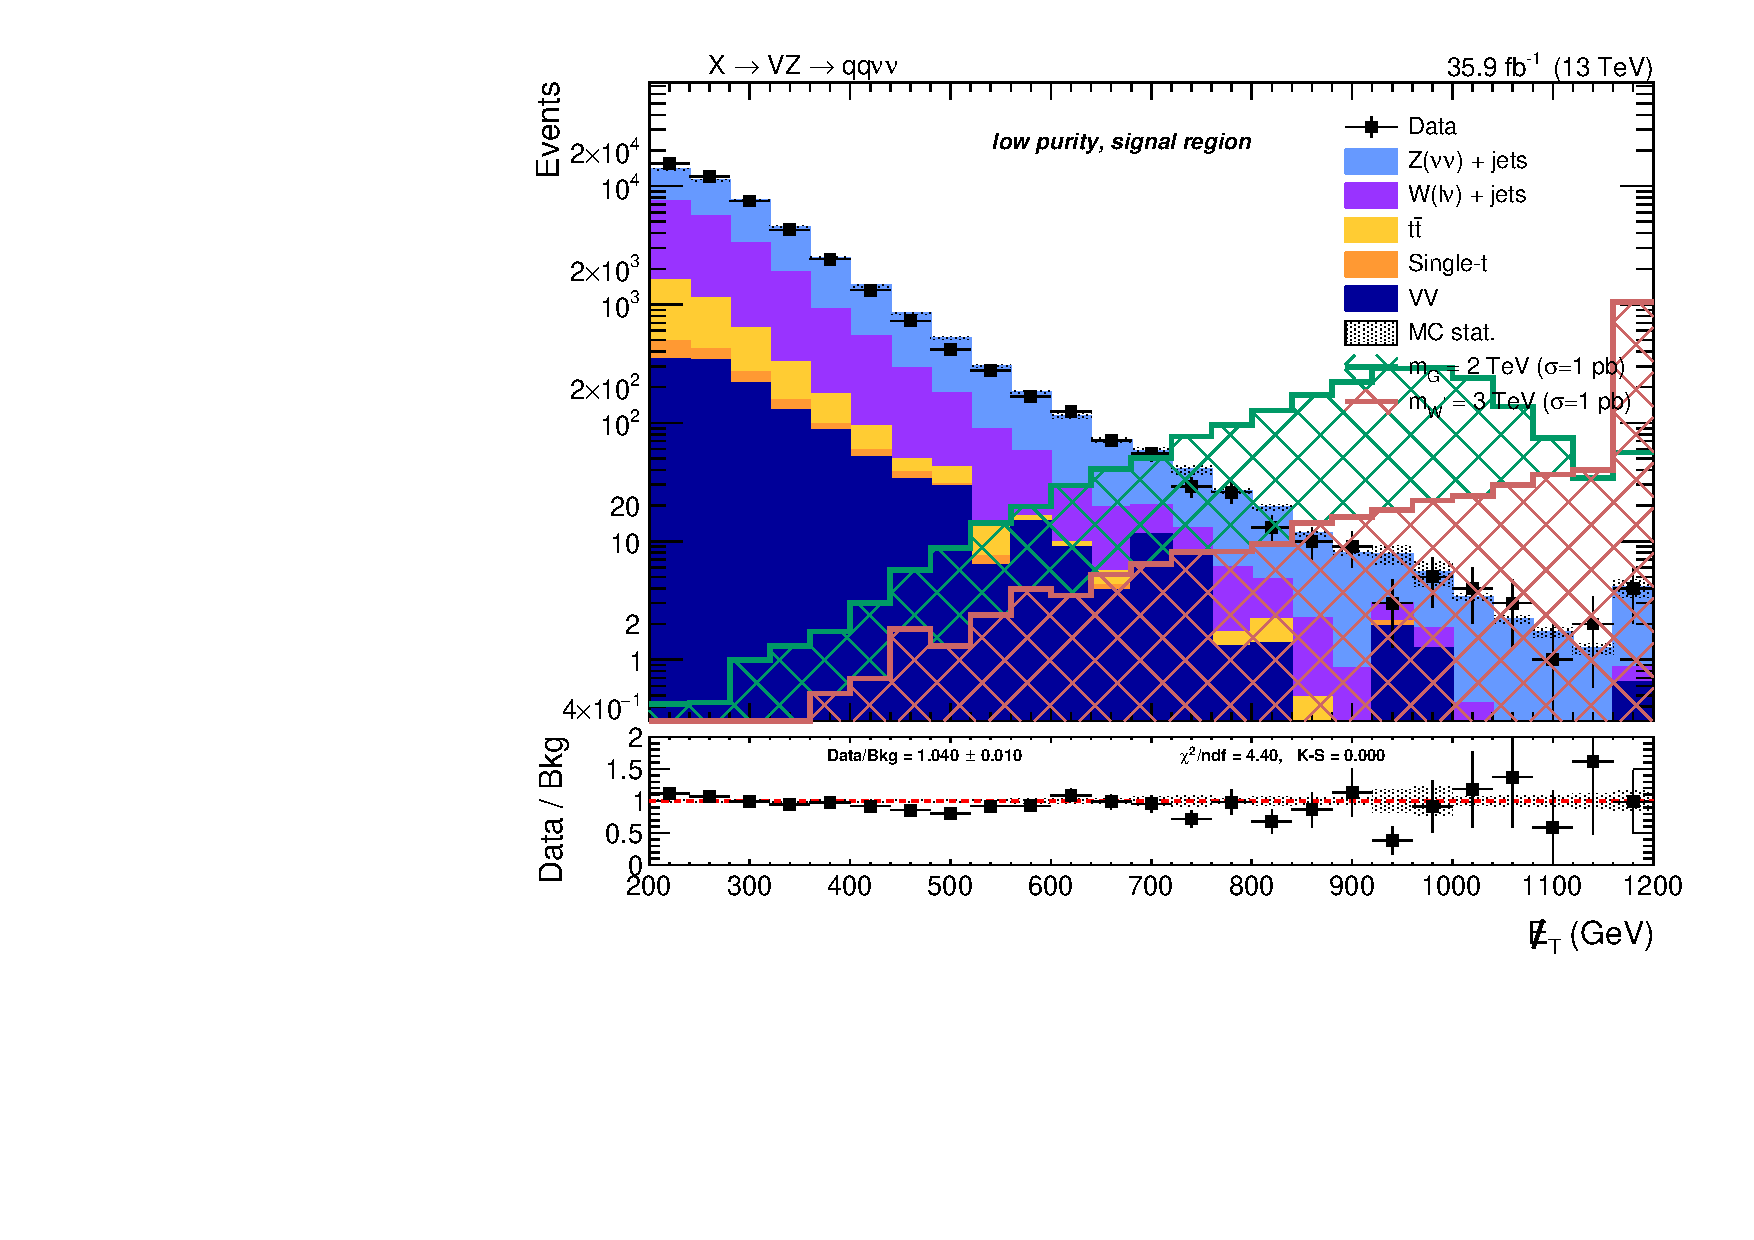
\includegraphics[width=0.495\textwidth]{plots/v9_thesis/XVZnnlpSR/MEt_pt.pdf}

    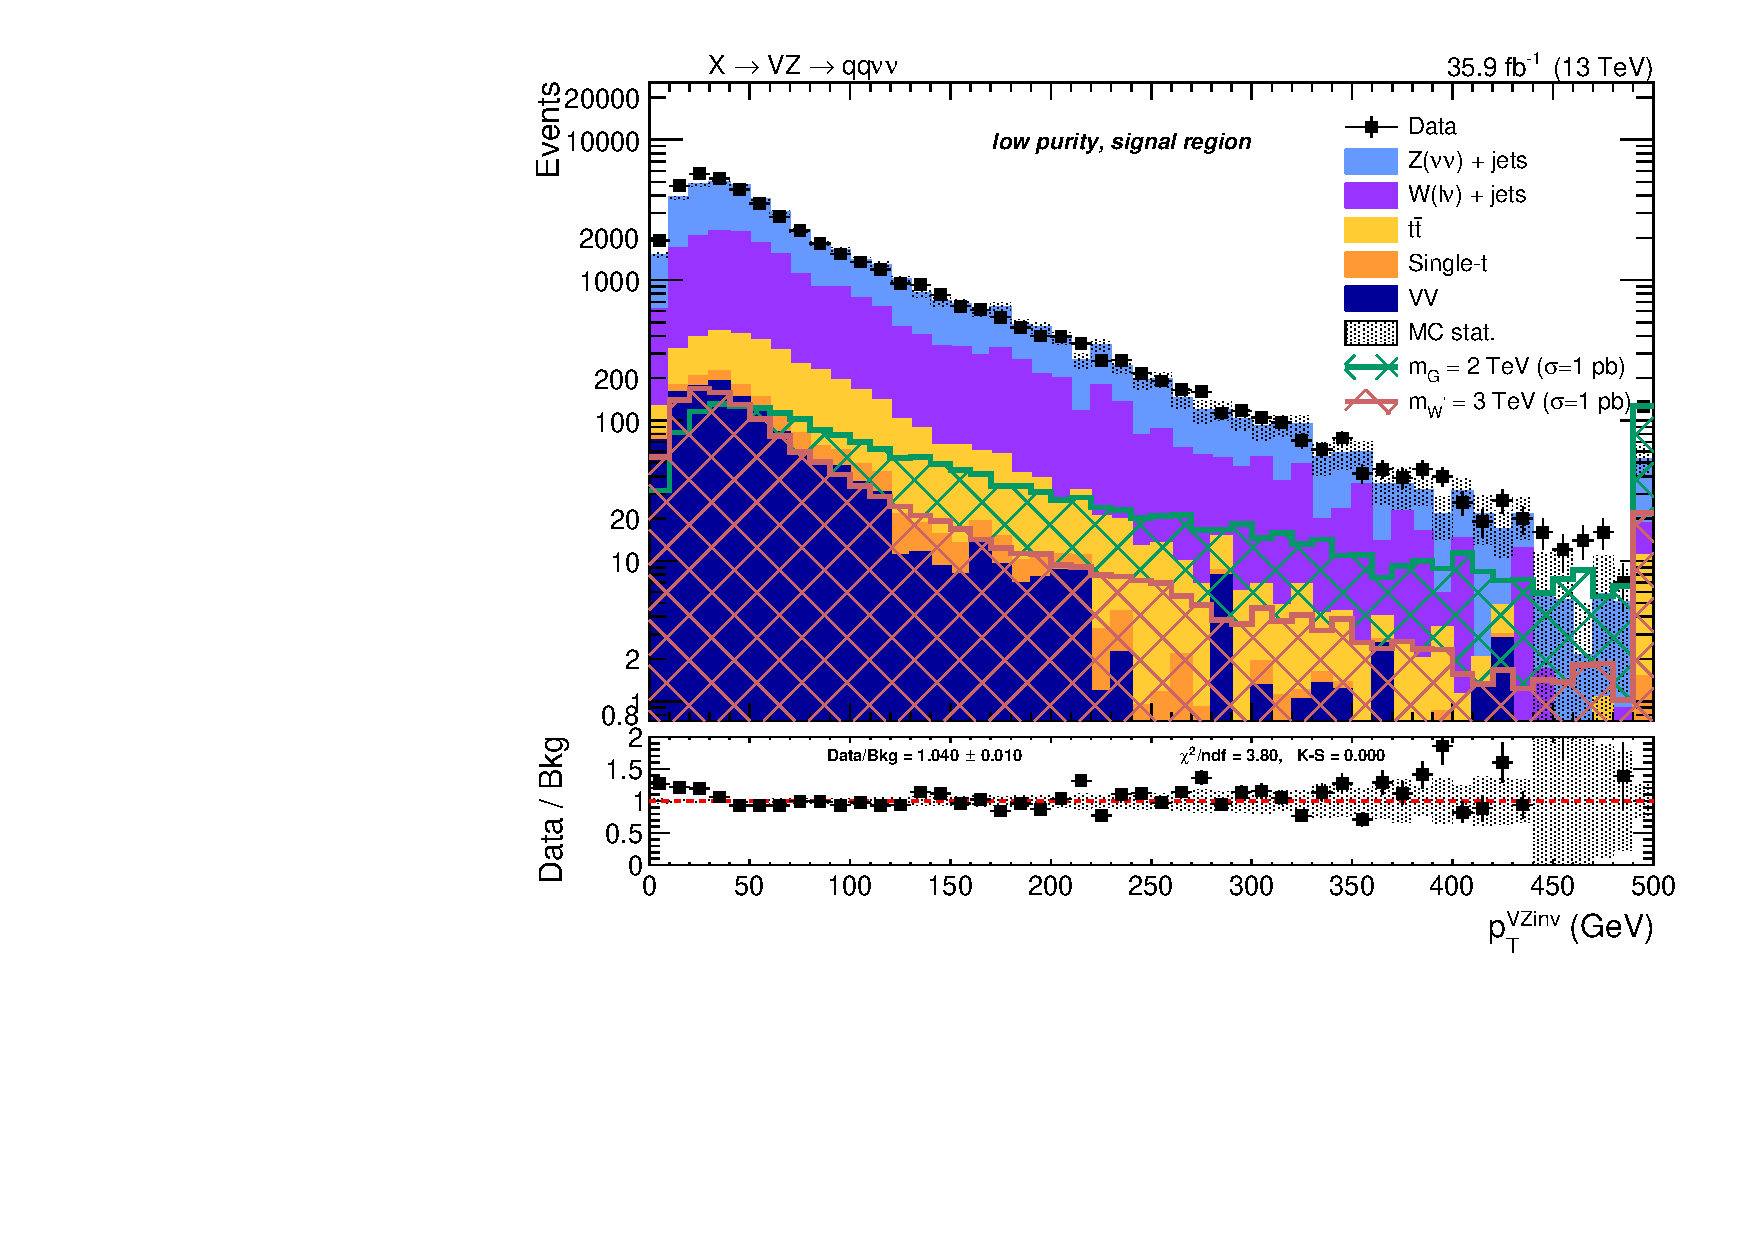
\includegraphics[width=0.495\textwidth]{plots/v9_thesis/XVZnnlpSR/X_pt.pdf}
    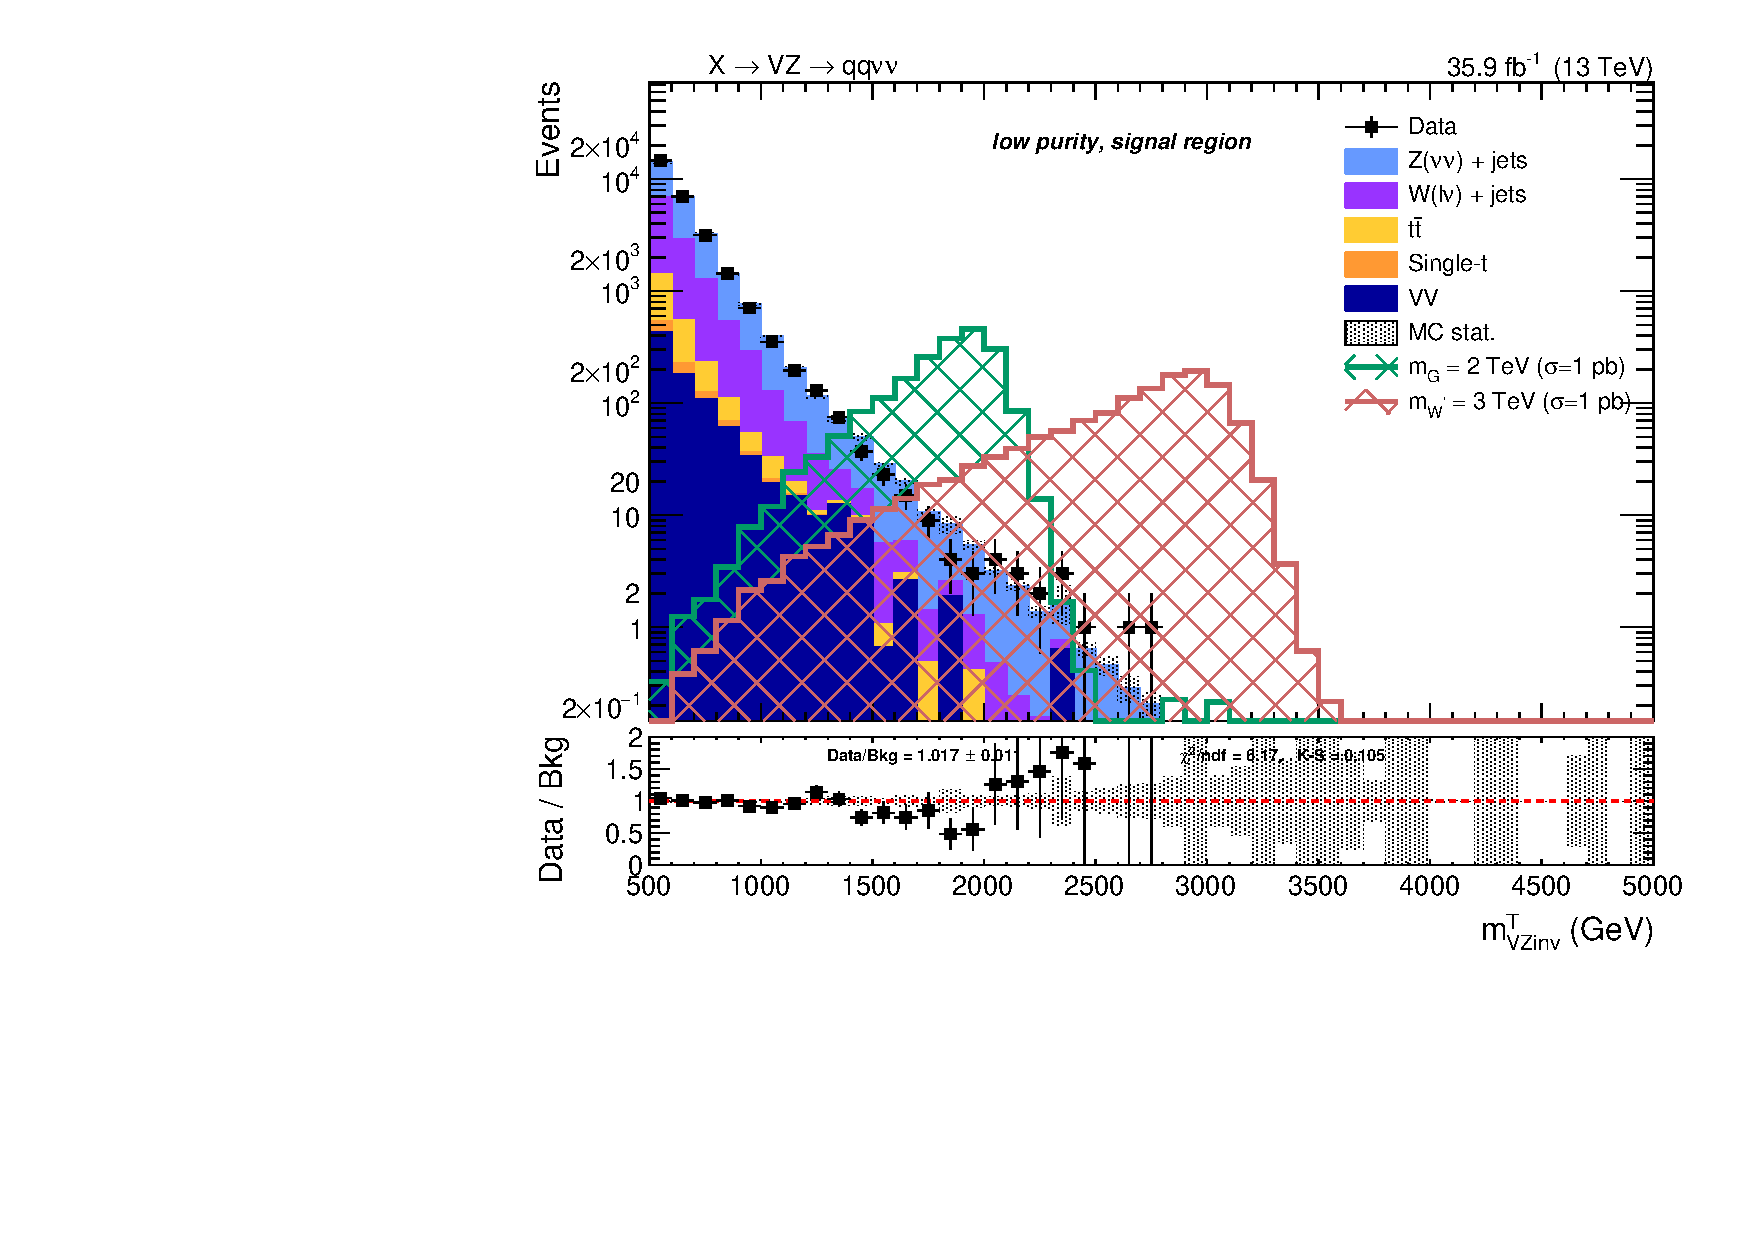
\includegraphics[width=0.495\textwidth]{plots/v9_thesis/XVZnnlpSR/X_tmass.pdf}

    \caption{Top: number of reconstructed primary vertices (left) and number of AK4 jets in the event (right). Center: distribution of the b-tagging multivariate discriminant for the AK4 jets not included in the \V jet cone (left) and \MET distribution (right). Bottom: \pt of the \VZ candidate (left) and transverse mass of the \VZ candidate (right). Events are selected with the \emph{low-purity signal region} selection, and simulated backgrounds are normalized to luminosity.}
%\label{fig:XZhll_N}
  \end{center}
\end{figure}

\clearpage

%plot scelti
%hpSR

\begin{figure}[!htb]
  \begin{center}
    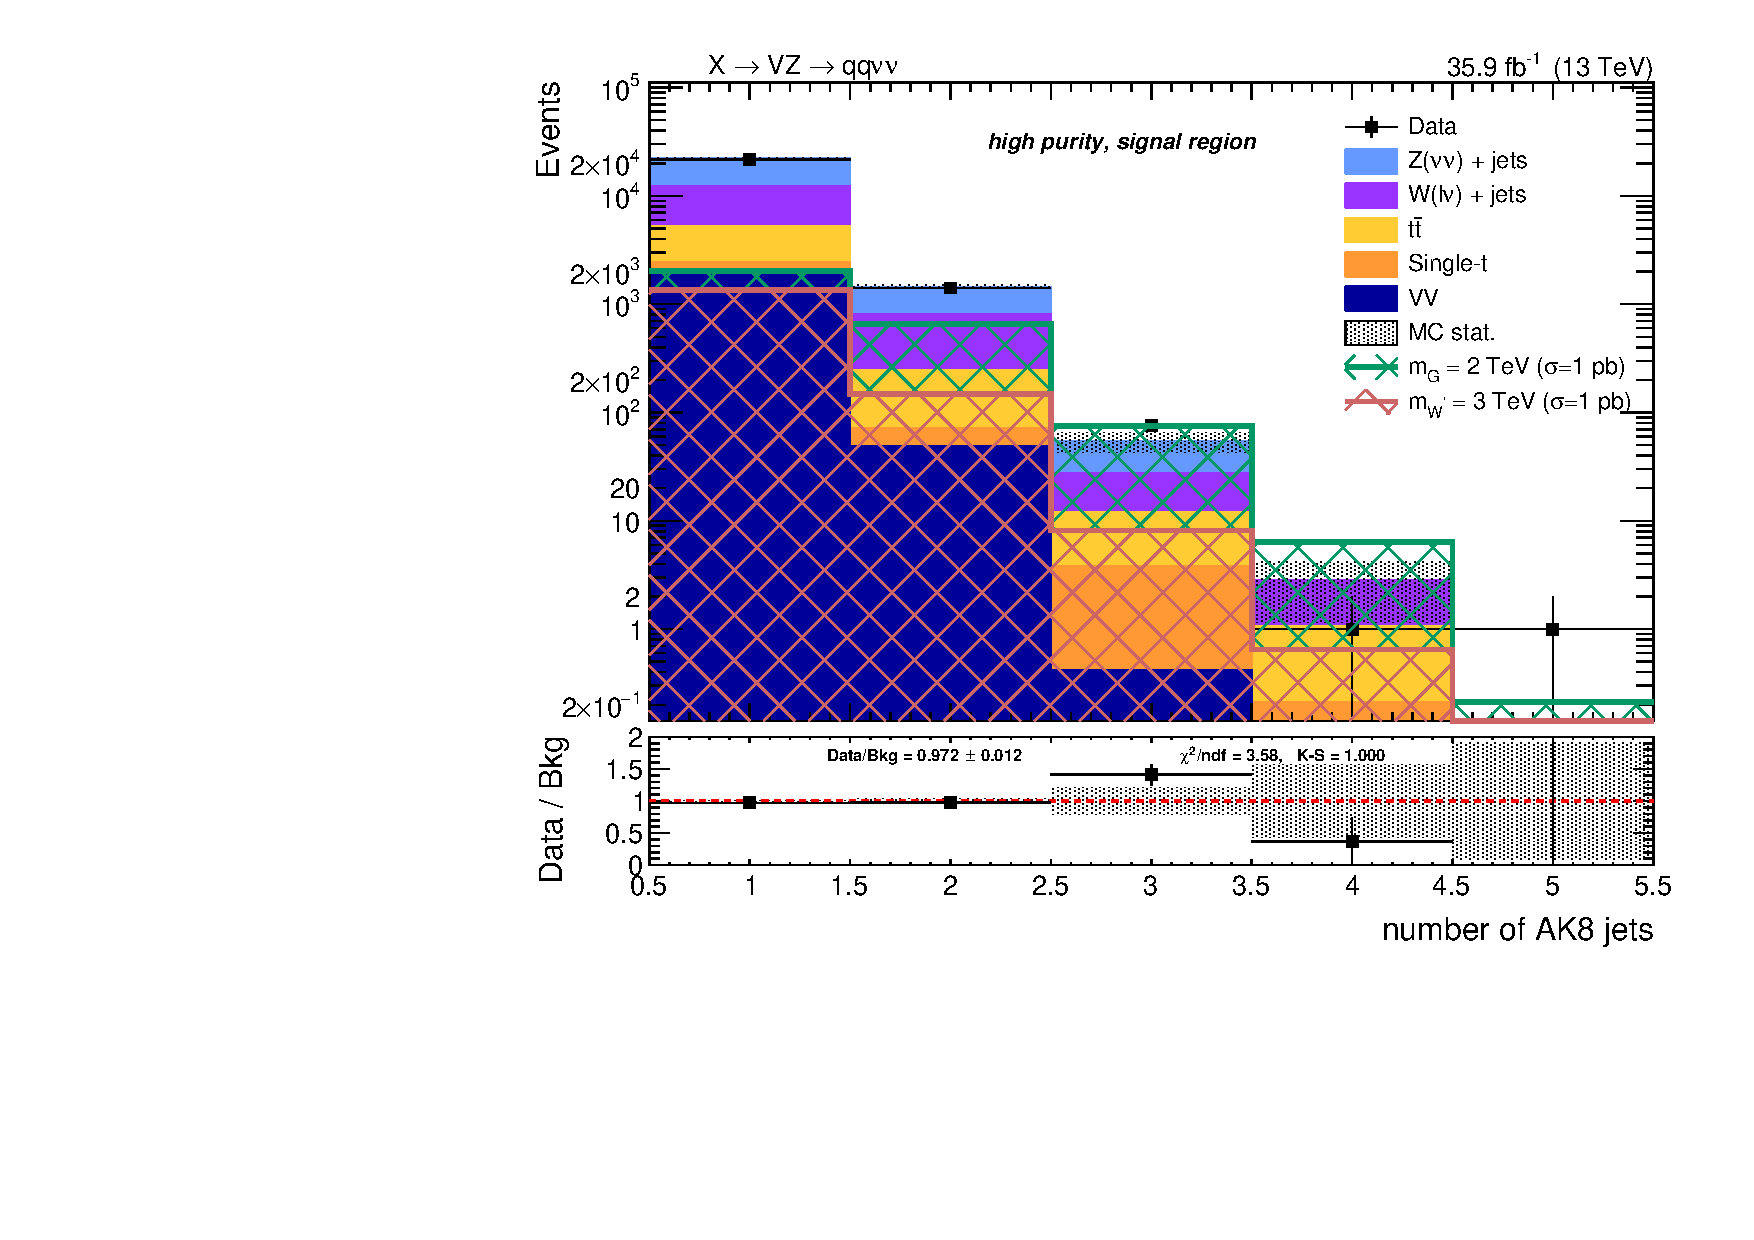
\includegraphics[width=0.495\textwidth]{plots/v9_thesis/XVZnnhpSR/nFatJets.pdf}  
    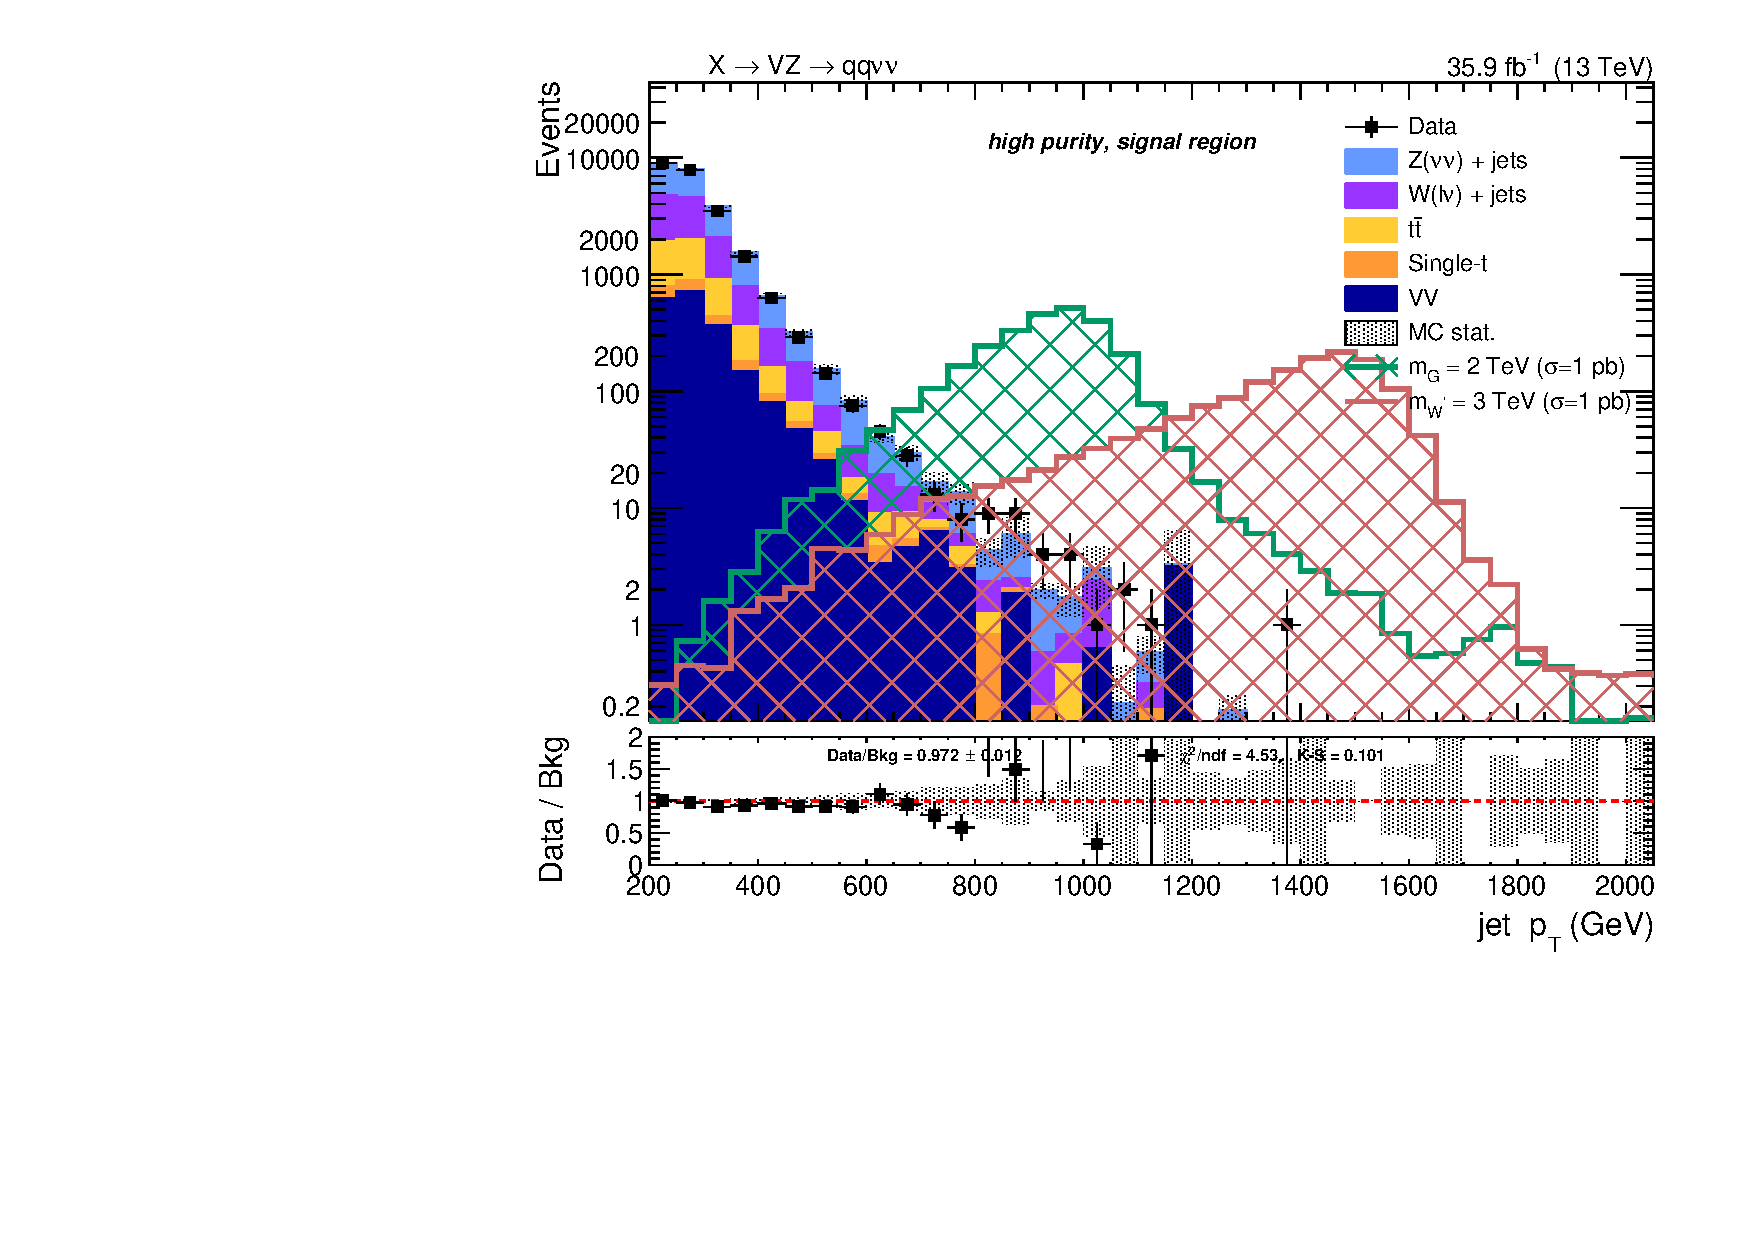
\includegraphics[width=0.495\textwidth]{plots/v9_thesis/XVZnnhpSR/FatJet1_pt.pdf}
    
    \includegraphics[width=0.495\textwidth]{plots/v9_thesis/XVZnnhpSR/FatJet1_eta.pdf}
    \includegraphics[width=0.495\textwidth]{plots/v9_thesis/XVZnnhpSR/FatJet1_dR.pdf}

    \includegraphics[width=0.495\textwidth]{plots/v9_thesis/XVZnnhpSR/FatJet1_puppiTau21.pdf}
    \includegraphics[width=0.495\textwidth]{plots/v9_thesis/XVZnnhpSR/FatJet1_softdropPuppiMassCorr.pdf}

    \caption{Top: number of AK8 jets in the event (left) and \V jet candidate \pt (right). Center: \V jet candidate $\eta$ (left) and angular separation $\Delta R$ between the constituents leading subjets (right). Bottom: \V jet candidate $\tau_{21}$ subjettiness after PUPPI correction (left) and \V jet candidate soft drop PUPPI mass (right). Events are selected with the \emph{high-purity signal region} selection, and simulated backgrounds are normalized to luminosity.}
%\label{fig:XZhll_N}
  \end{center}
\end{figure}

\clearpage

\begin{figure}[!htb]
  \begin{center}  
    \includegraphics[width=0.495\textwidth]{plots/v9_thesis/XVZnnhpSR/nPV.pdf}
    \includegraphics[width=0.495\textwidth]{plots/v9_thesis/XVZnnhpSR/nJets.pdf}

    \includegraphics[width=0.495\textwidth]{plots/v9_thesis/XVZnnhpSR/MaxJetBTag.pdf}
    \includegraphics[width=0.495\textwidth]{plots/v9_thesis/XVZnnhpSR/MEt_pt.pdf}

    \includegraphics[width=0.495\textwidth]{plots/v9_thesis/XVZnnhpSR/X_pt.pdf}
    \includegraphics[width=0.495\textwidth]{plots/v9_thesis/XVZnnhpSR/X_tmass.pdf}

    \caption{Top: number of reconstructed primary vertices (left) and number of AK4 jets in the event (right). Center: distribution of the b-tagging multivariate discriminant for the AK4 jets not included in the \V jet cone (left) and \MET distribution (right). Bottom: \pt of the \VZ candidate (left) and transverse mass of the \VZ candidate (right). Events are selected with the \emph{high-purity signal region} selection, and simulated backgrounds are normalized to luminosity.}
\label{fig:plot_last}
  \end{center}
\end{figure}



